\chapter{คู่มือการใช้งานระบบ}
คู่มือการใช้งานทั้งหมดของระบบ สามารถแบ่งออกเป็น 2 ส่วน ดังนี้
\begin{enumerate}
	\item ส่วนของหน้าเมนูแอปพลิเคชันสำหรับนักศึกษา
		\begin{itemize}
			\item หน้าจอต้อนรับแสดงผลทุกครั้งเมื่อผู้ใช้ทำการเปิดใช้งานแอปพลิเคชัน ดังแสดงในรูปที่ \ref{Fig:open}
				\begin{figure}[H]
					\centering
					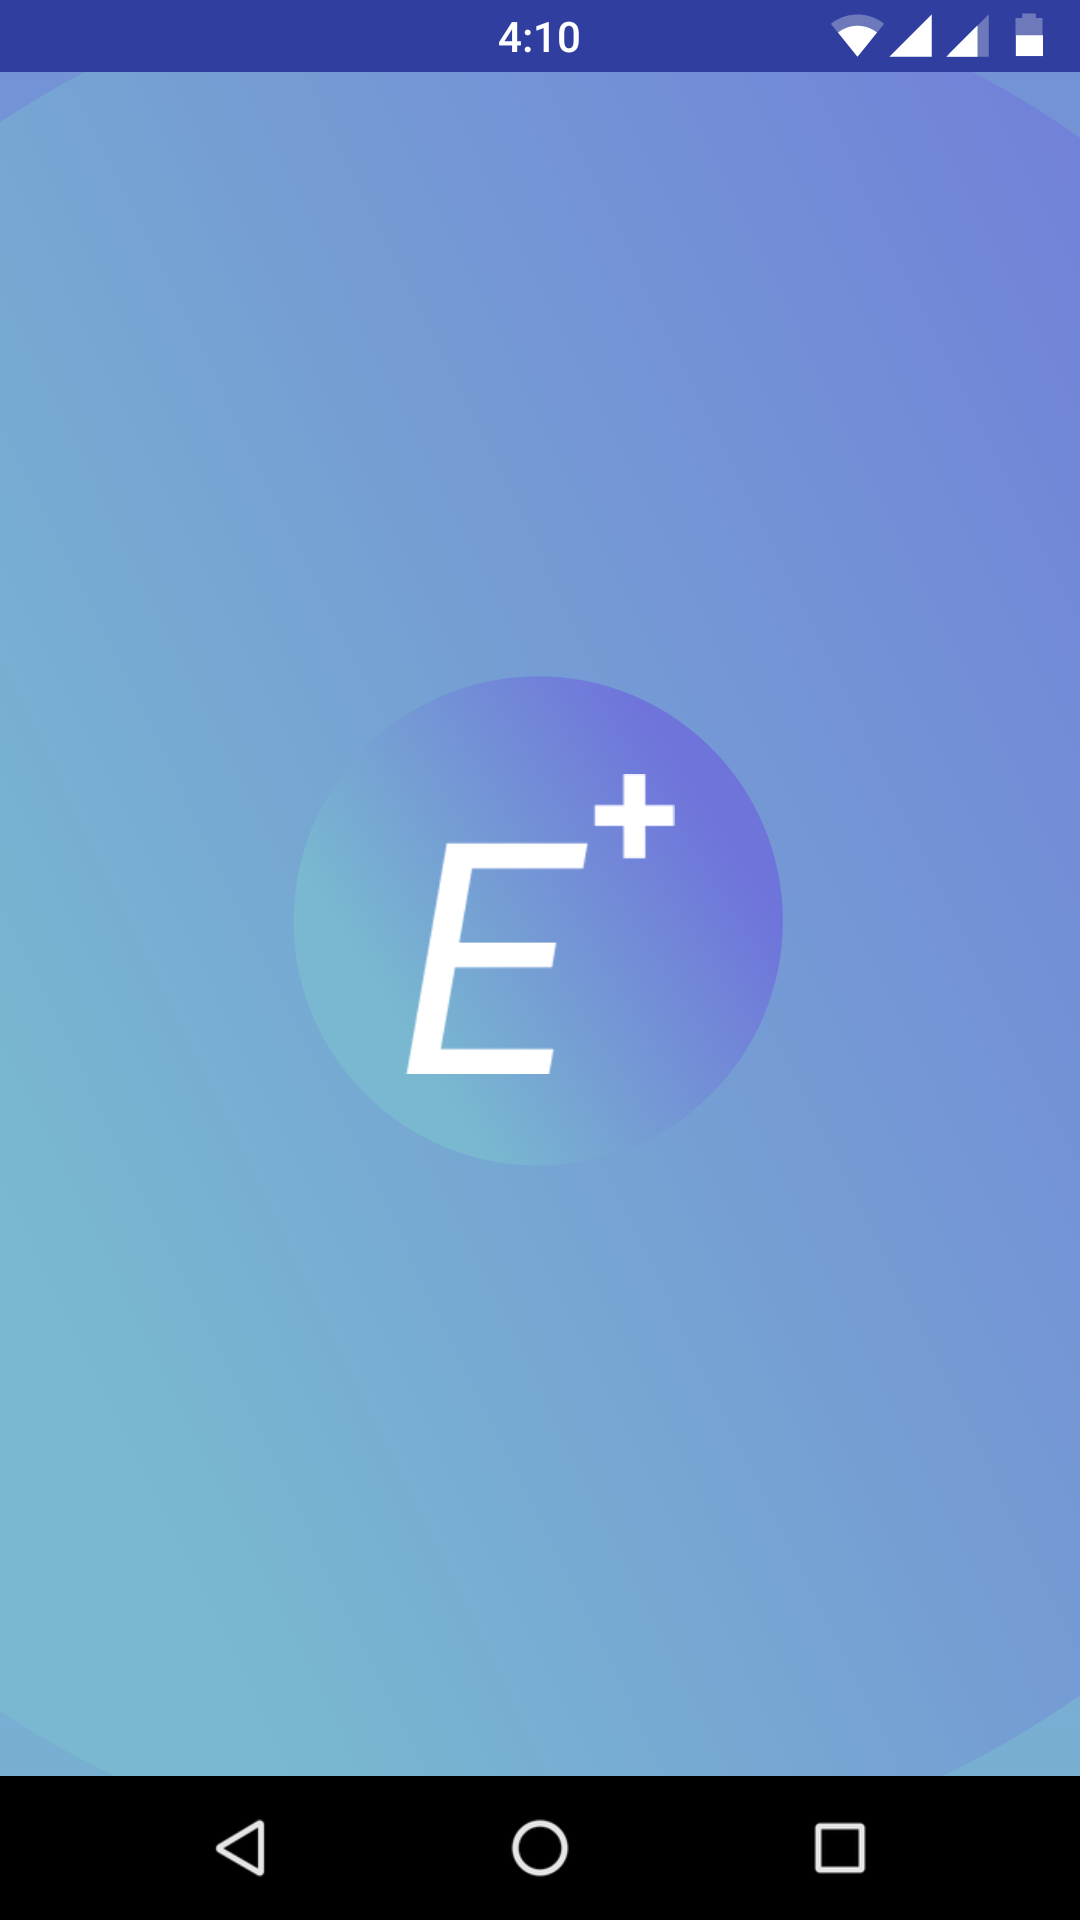
\includegraphics[width=0.3\columnwidth]{Figures/7/Manual/open}
					\caption{หน้าจอต้อนรับ}
					\label{Fig:open}
				\end{figure}
			
			\item เมื่อระบบทำการตรวจสอบว่ามีสิทธิ์(Permission)ในการใช้งานแอปพลิเคชันที่ผู้ใช้ยังไม่ได้อนุญาตให้เข้าถึง ระบบจะแสดงหน้าต่างขอสิทธิ์การเข้าถึง ดังแสดงในรูปที่ \ref{Fig:permission}
			\begin{figure}[H]
				\centering
				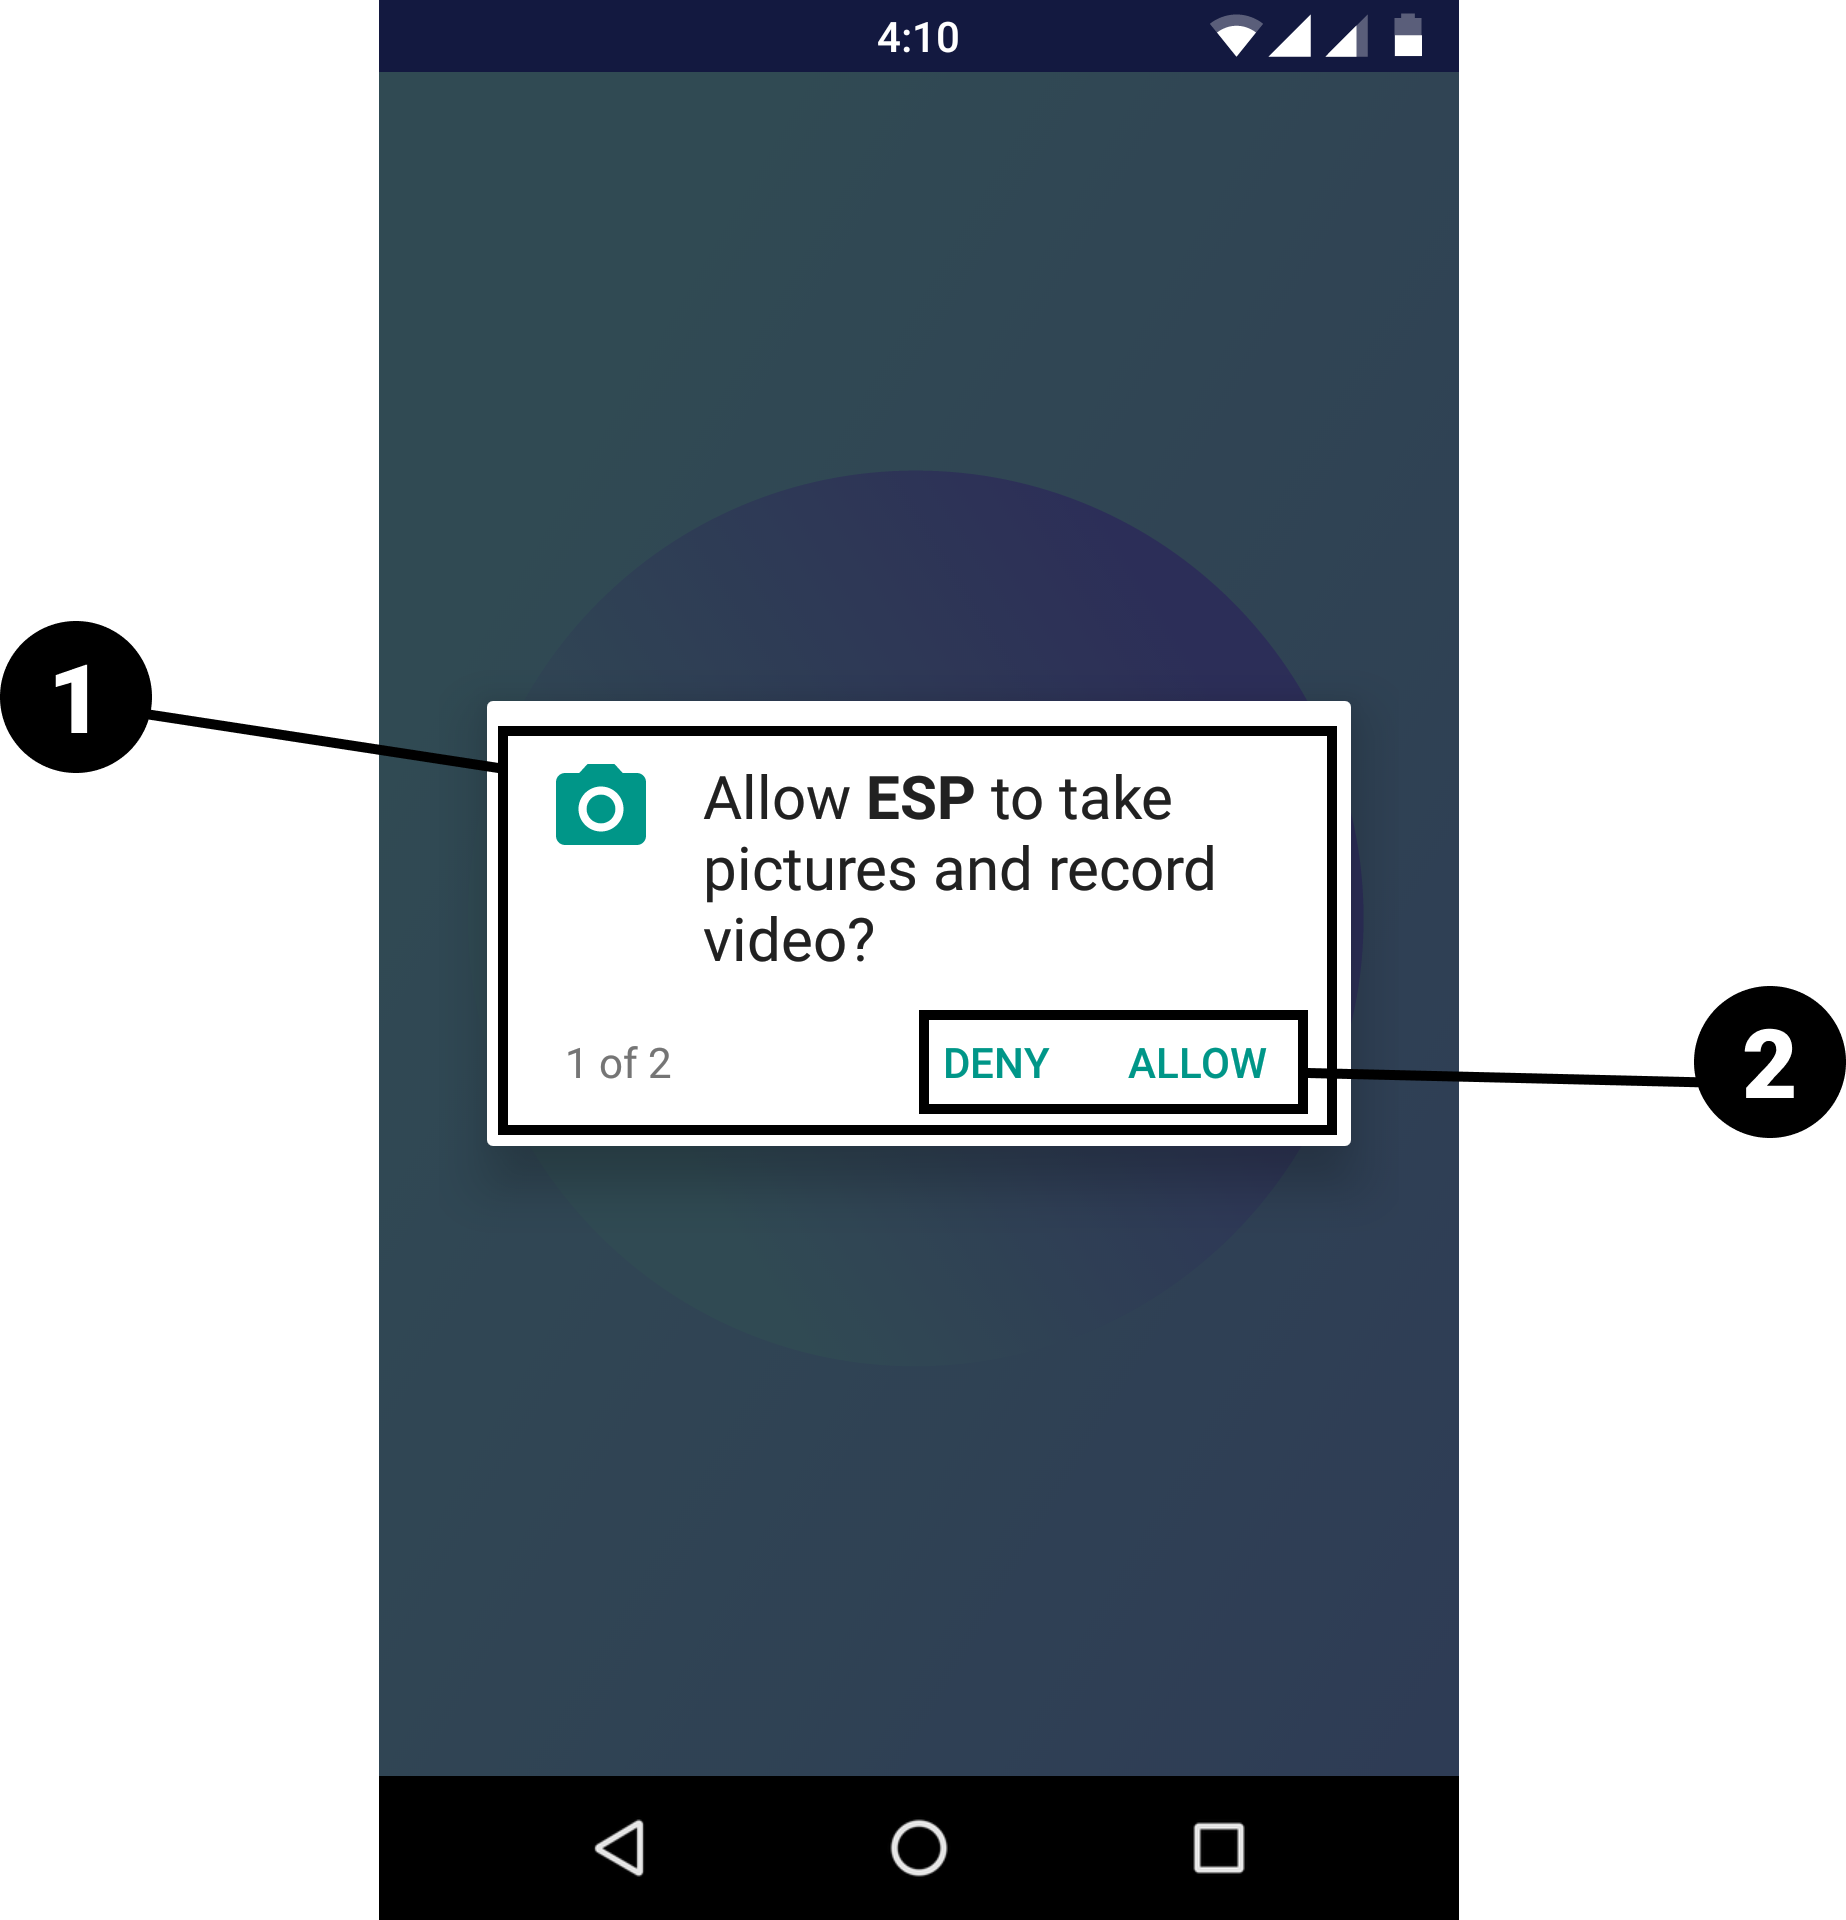
\includegraphics[width=0.5\columnwidth]{Figures/7/Manual/permission}
				\caption{หน้าต่างขอสิทธิ์การเข้าถึง}
				\label{Fig:permission}
			\end{figure}
		จากรูปที่ \ref{Fig:permission} สามารถอธิบายการใช้งานได้ดังนี้
			\begin{itemize}[label={--}]
				\item หมายเลข 1 คือ หน้าต่างขอสิทธิ์การเข้าถึงข้อมูล
				\item หมายเลข 2 คือ ปุ่มให้สิทธิ์และยกเลิกการให้สิทธิ์
			\end{itemize}
			
			\item ระบบทำการตรวจสอบทุกครั้งเมื่อผู้ใช้งานเปิดใช้งานแอปพลิเคชัน หากผู้ใช้งานคนปัจจุบันยังไม่ได้เข้าสู่ระบบ ระบบจะแสดงหน้าจอเข้าสู่ระบบโดยผู้ใช้งานจำเป็นต้องทำการกรอกข้อมูลคือ อีเมลและรหัสผ่าน ดังแสดงในรูปที่ \ref{Fig:signin}
			\begin{figure}[H]
				\centering
				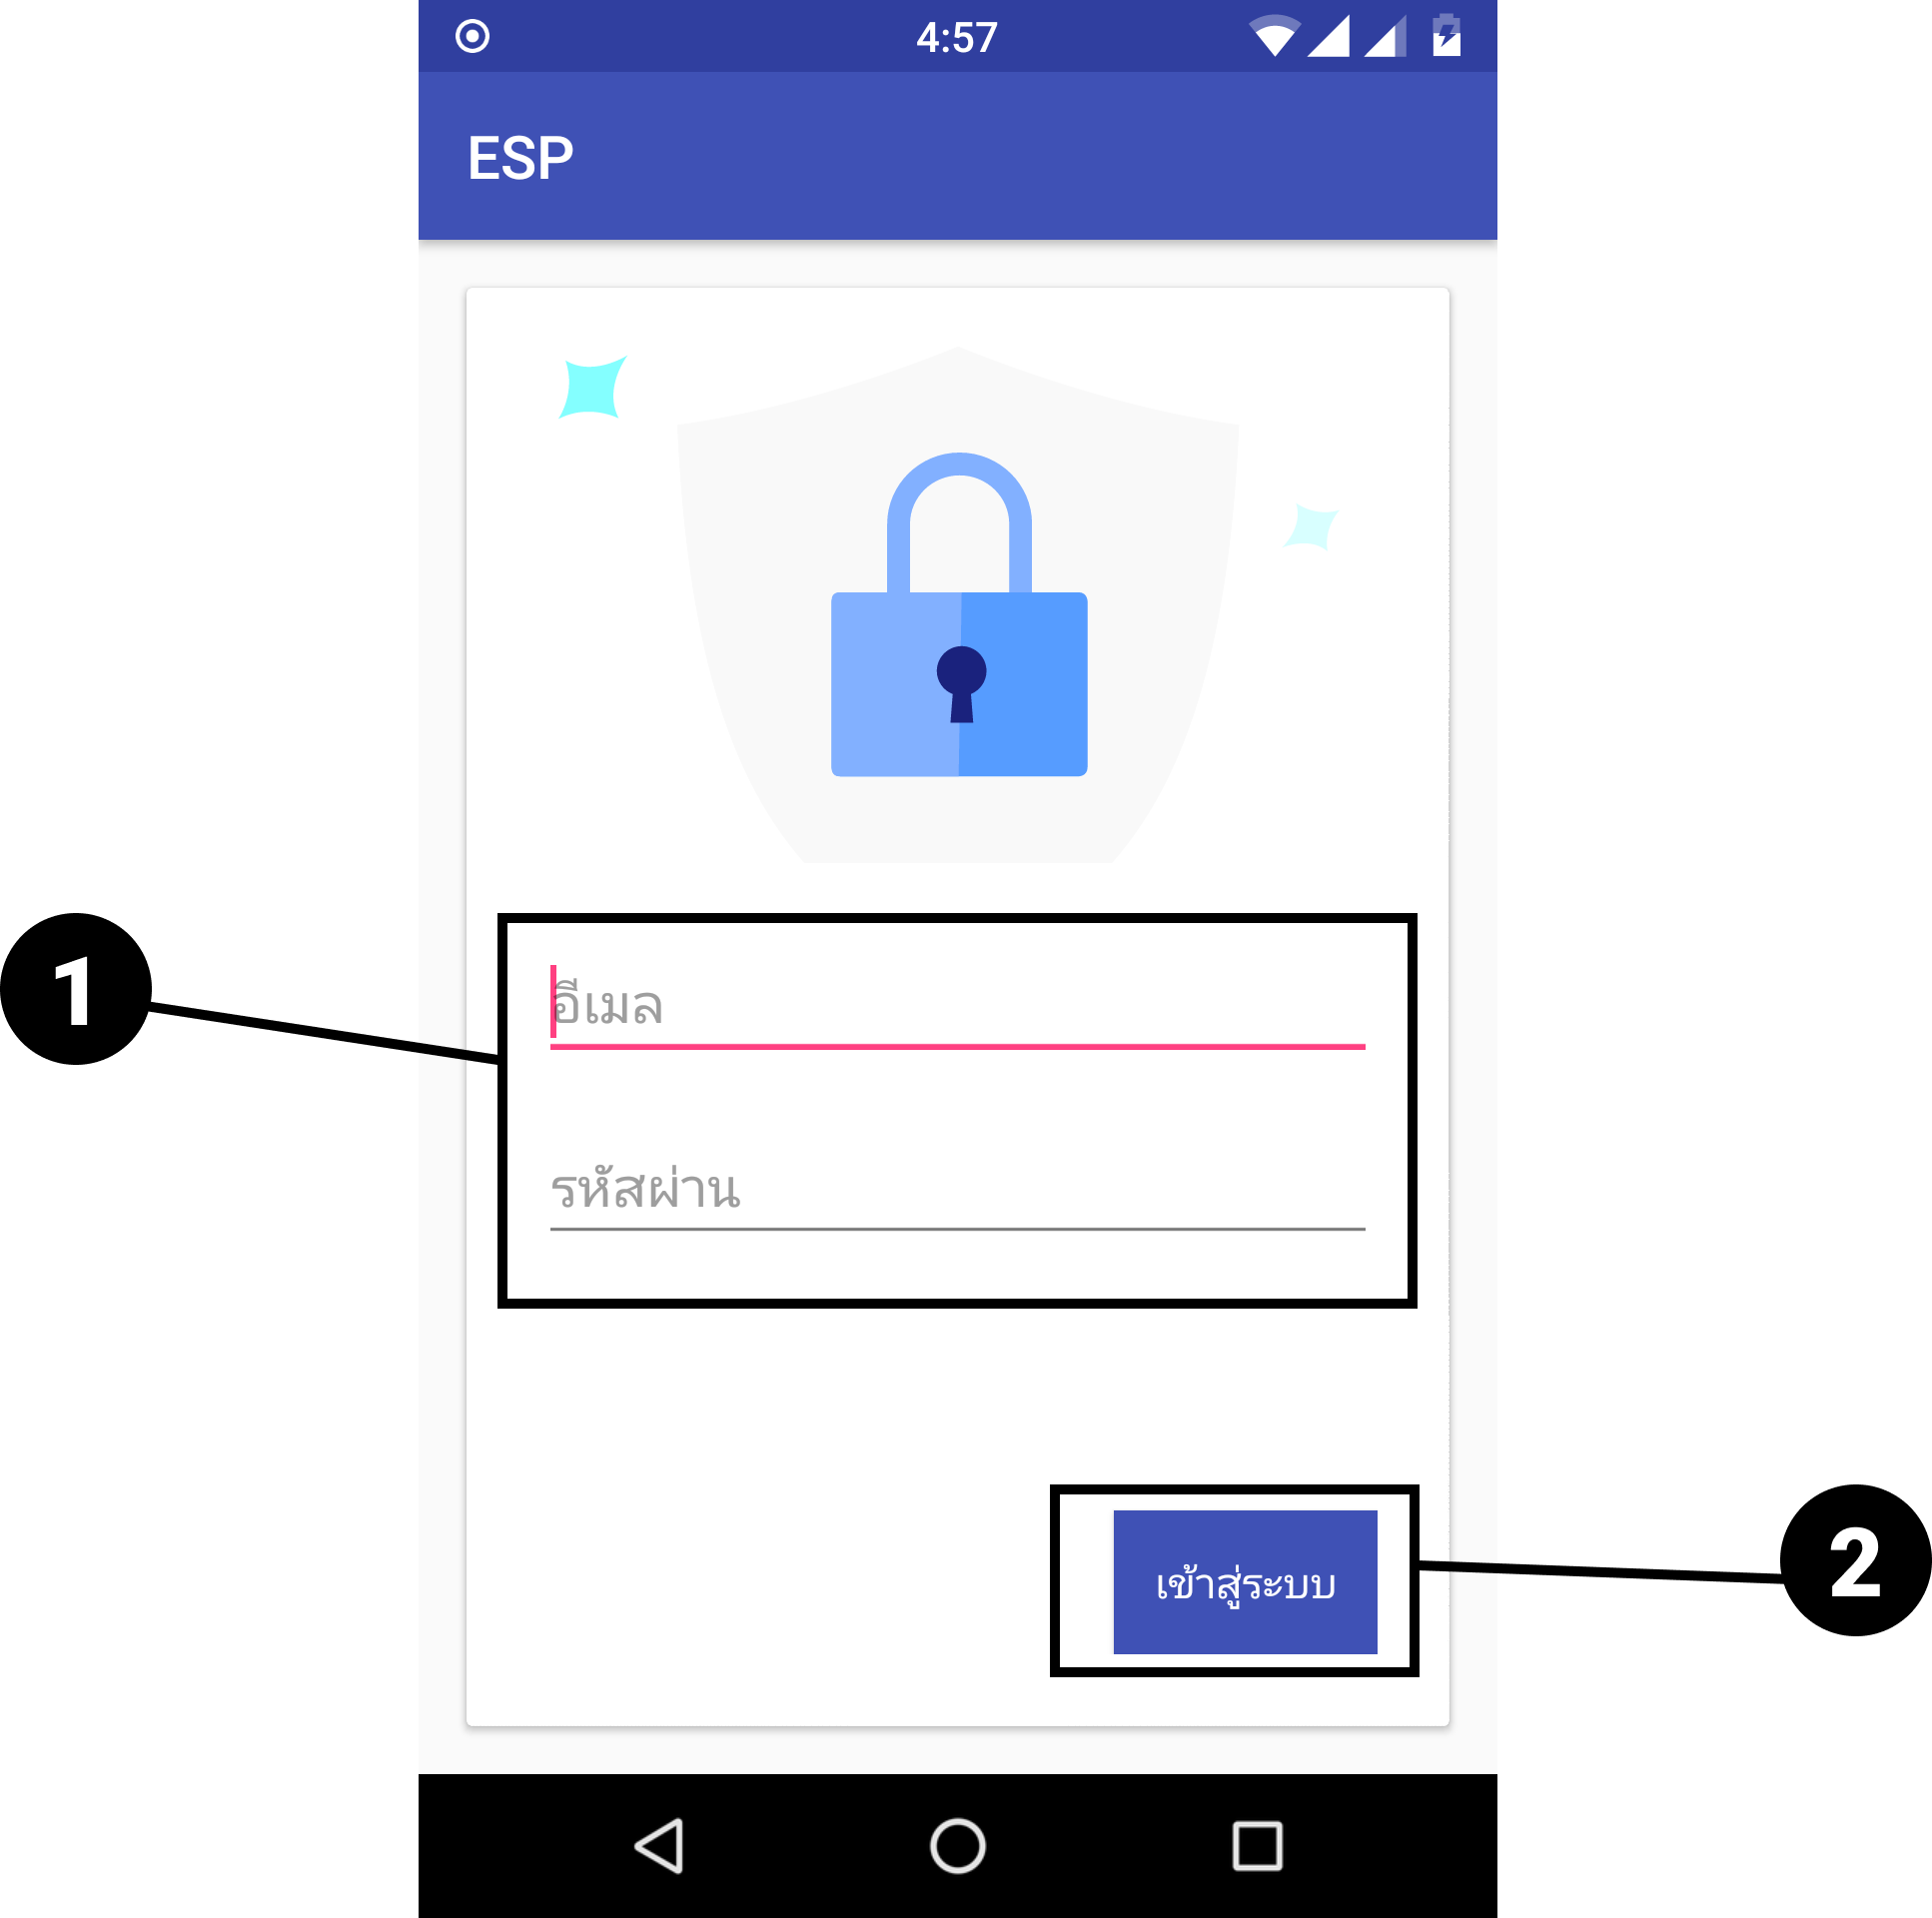
\includegraphics[width=0.5\columnwidth]{Figures/7/Manual/signin}
				\caption{หน้าจอเข้าสู่ระบบ}
				\label{Fig:signin}
			\end{figure}
			จากรูปที่ \ref{Fig:signin} สามารถอธิบายการใช้งานได้ดังนี้
			\begin{itemize}[label={--}]
				\item หมายเลข 1 คือ ส่วนของฟอร์มในการกรอกข้อมูลอีเมลและรหัสผ่าน
				\item หมายเลข 2 คือ ปุ่มกดเข้าสู่ระบบ
			\end{itemize}
		
			\item หน้าแสดงข่าวสารประชาสัมพันธ์ซึ่งเป็นหน้าจอหลักของแอปพลิเคชัน ดังแสดงในรูปที่ \ref{Fig:feed}
			\begin{figure}[H]
				\centering
				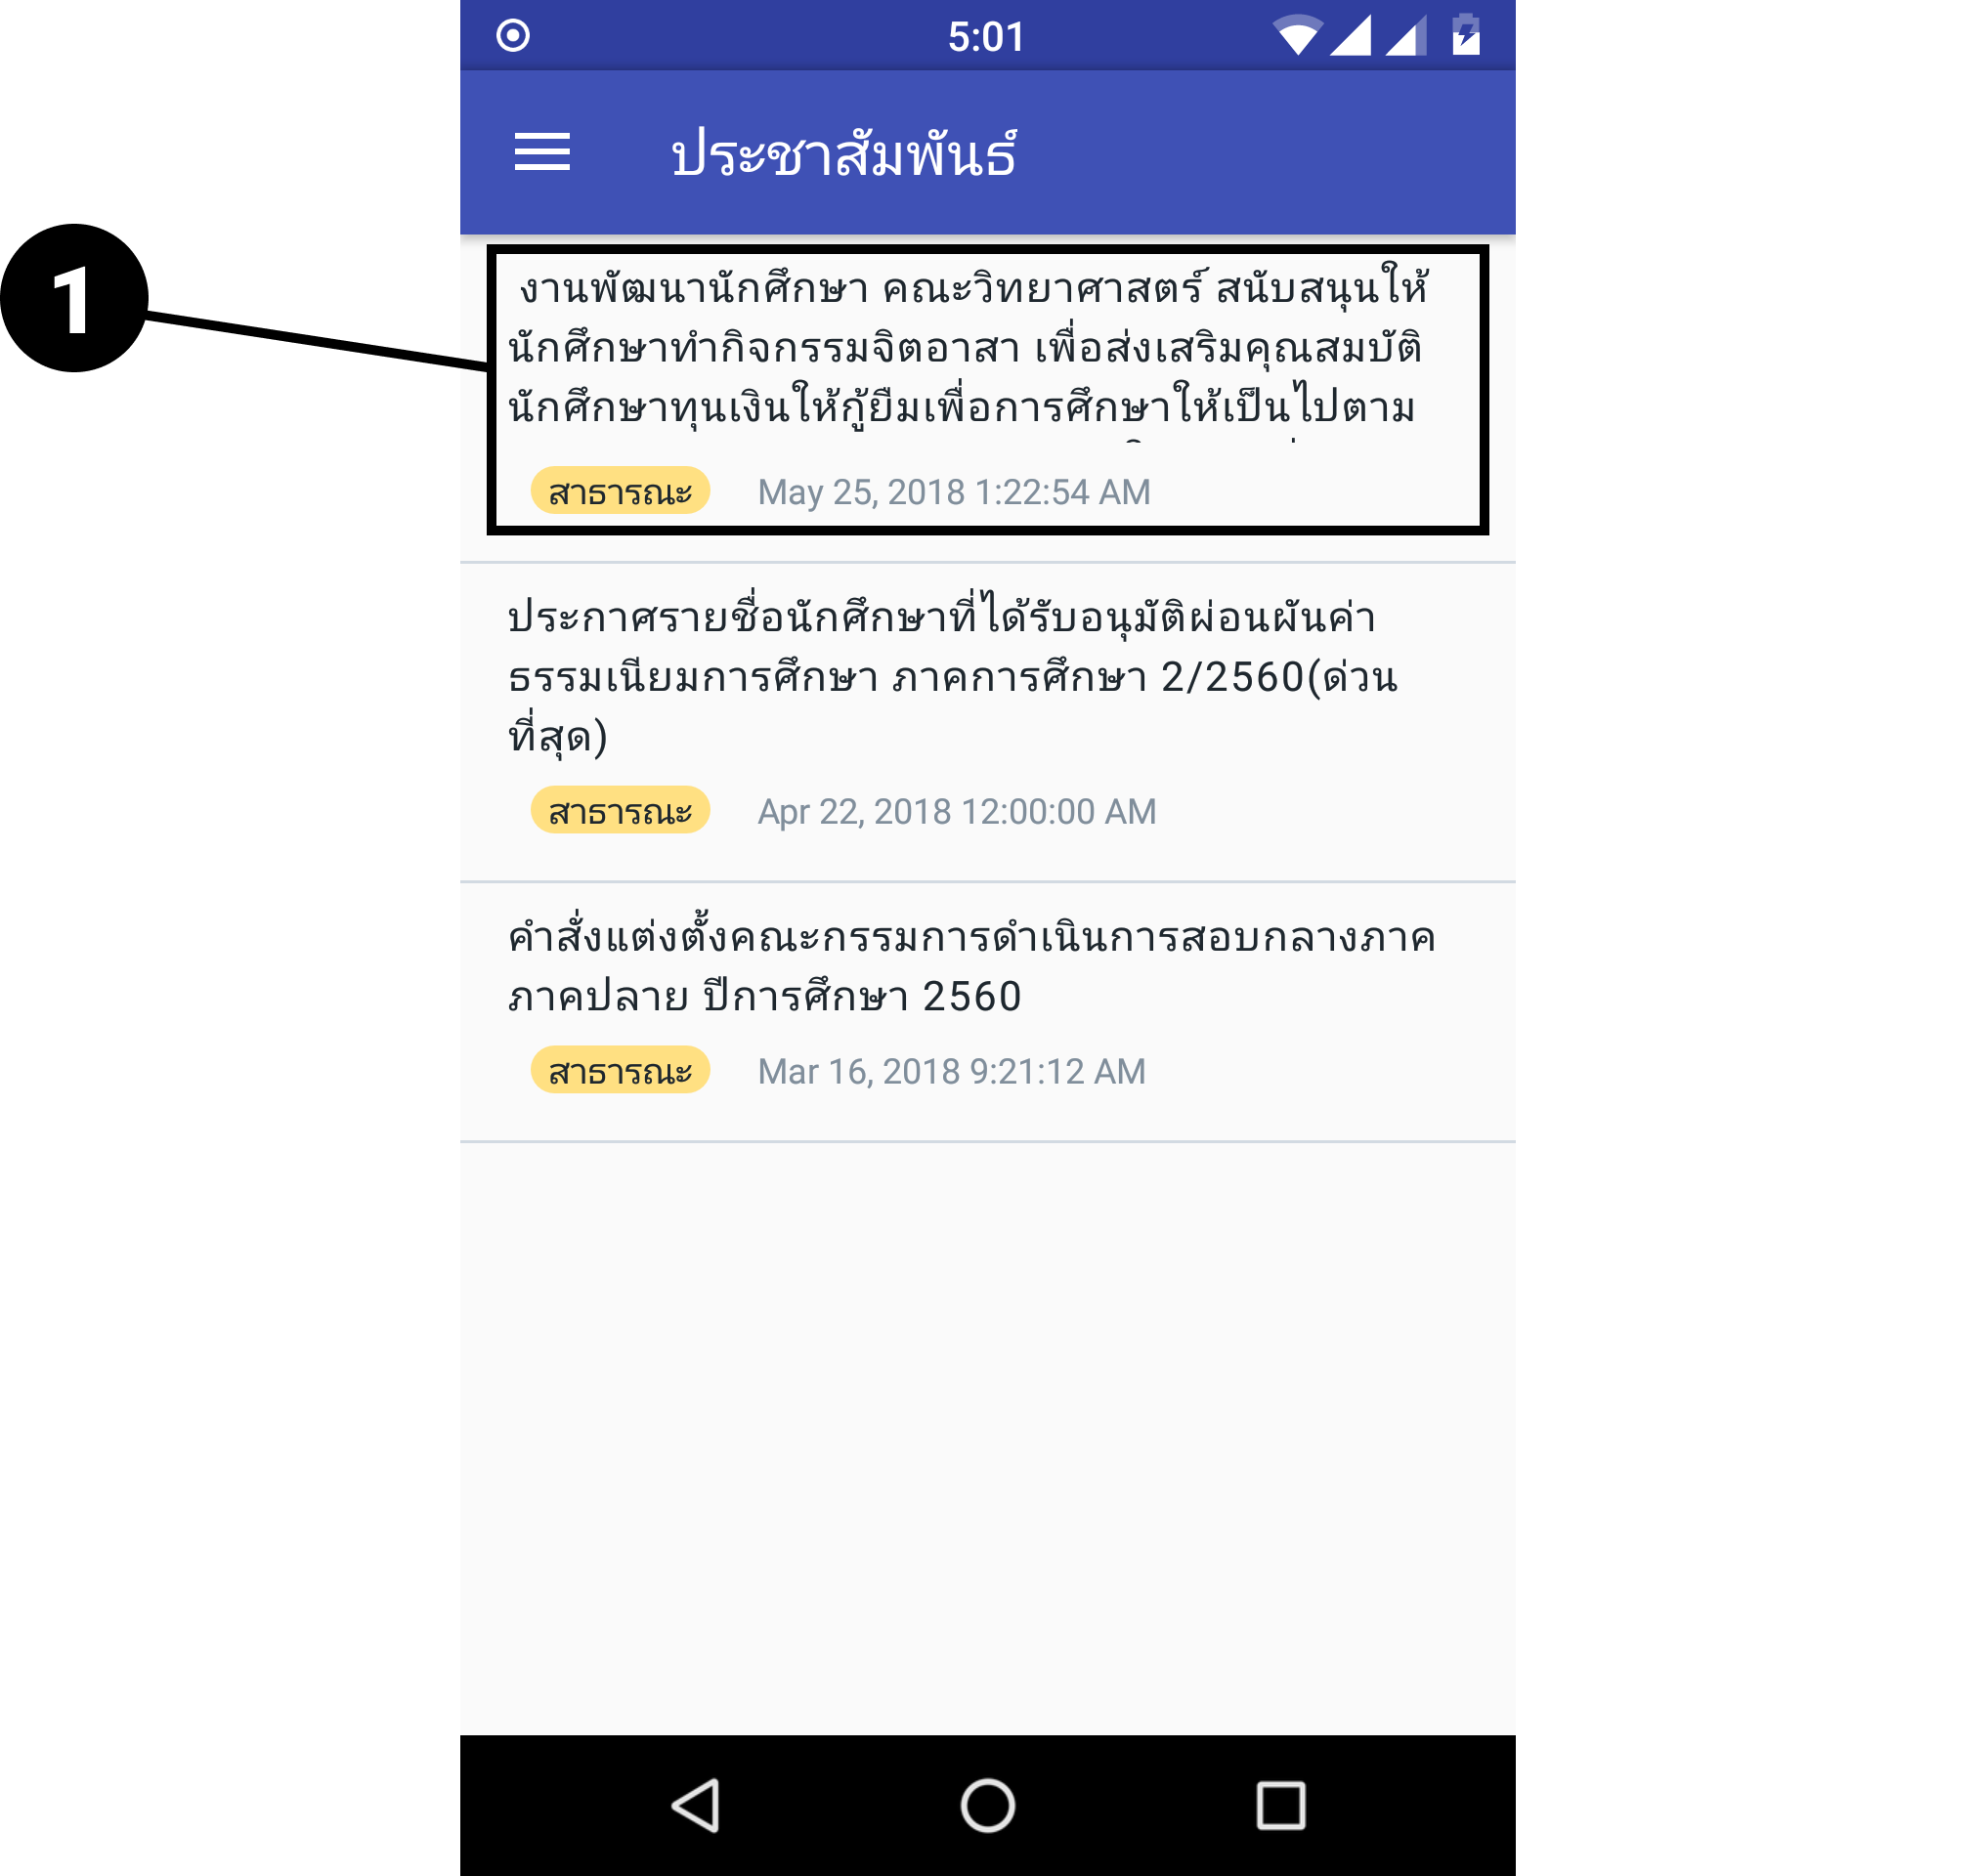
\includegraphics[width=0.5\columnwidth]{Figures/7/Manual/feed}
				\caption{หน้าแสดงข่าวสาร}
				\label{Fig:feed}
			\end{figure}
			จากรูปที่ \ref{Fig:feed} สามารถอธิบายการใช้งานได้ดังนี้
			\begin{itemize}[label={--}]
				\item หมายเลข 1 คือ ข่าวสารที่มีข้อมูล หัวข้อข่าวสาร แท็ก(Tag)และวันที่ประการข่าวสาร
			\end{itemize}
		
			\item เมื่อผู้ใช้กดเลือกดูรายละเอียดของข่าวสาร ระบบจะแสดงหน้าจอรายละเอียดข่าวสาร ดังแสดงในรูปที่ \ref{Fig:viewpost}
			\begin{figure}[H]
				\centering
				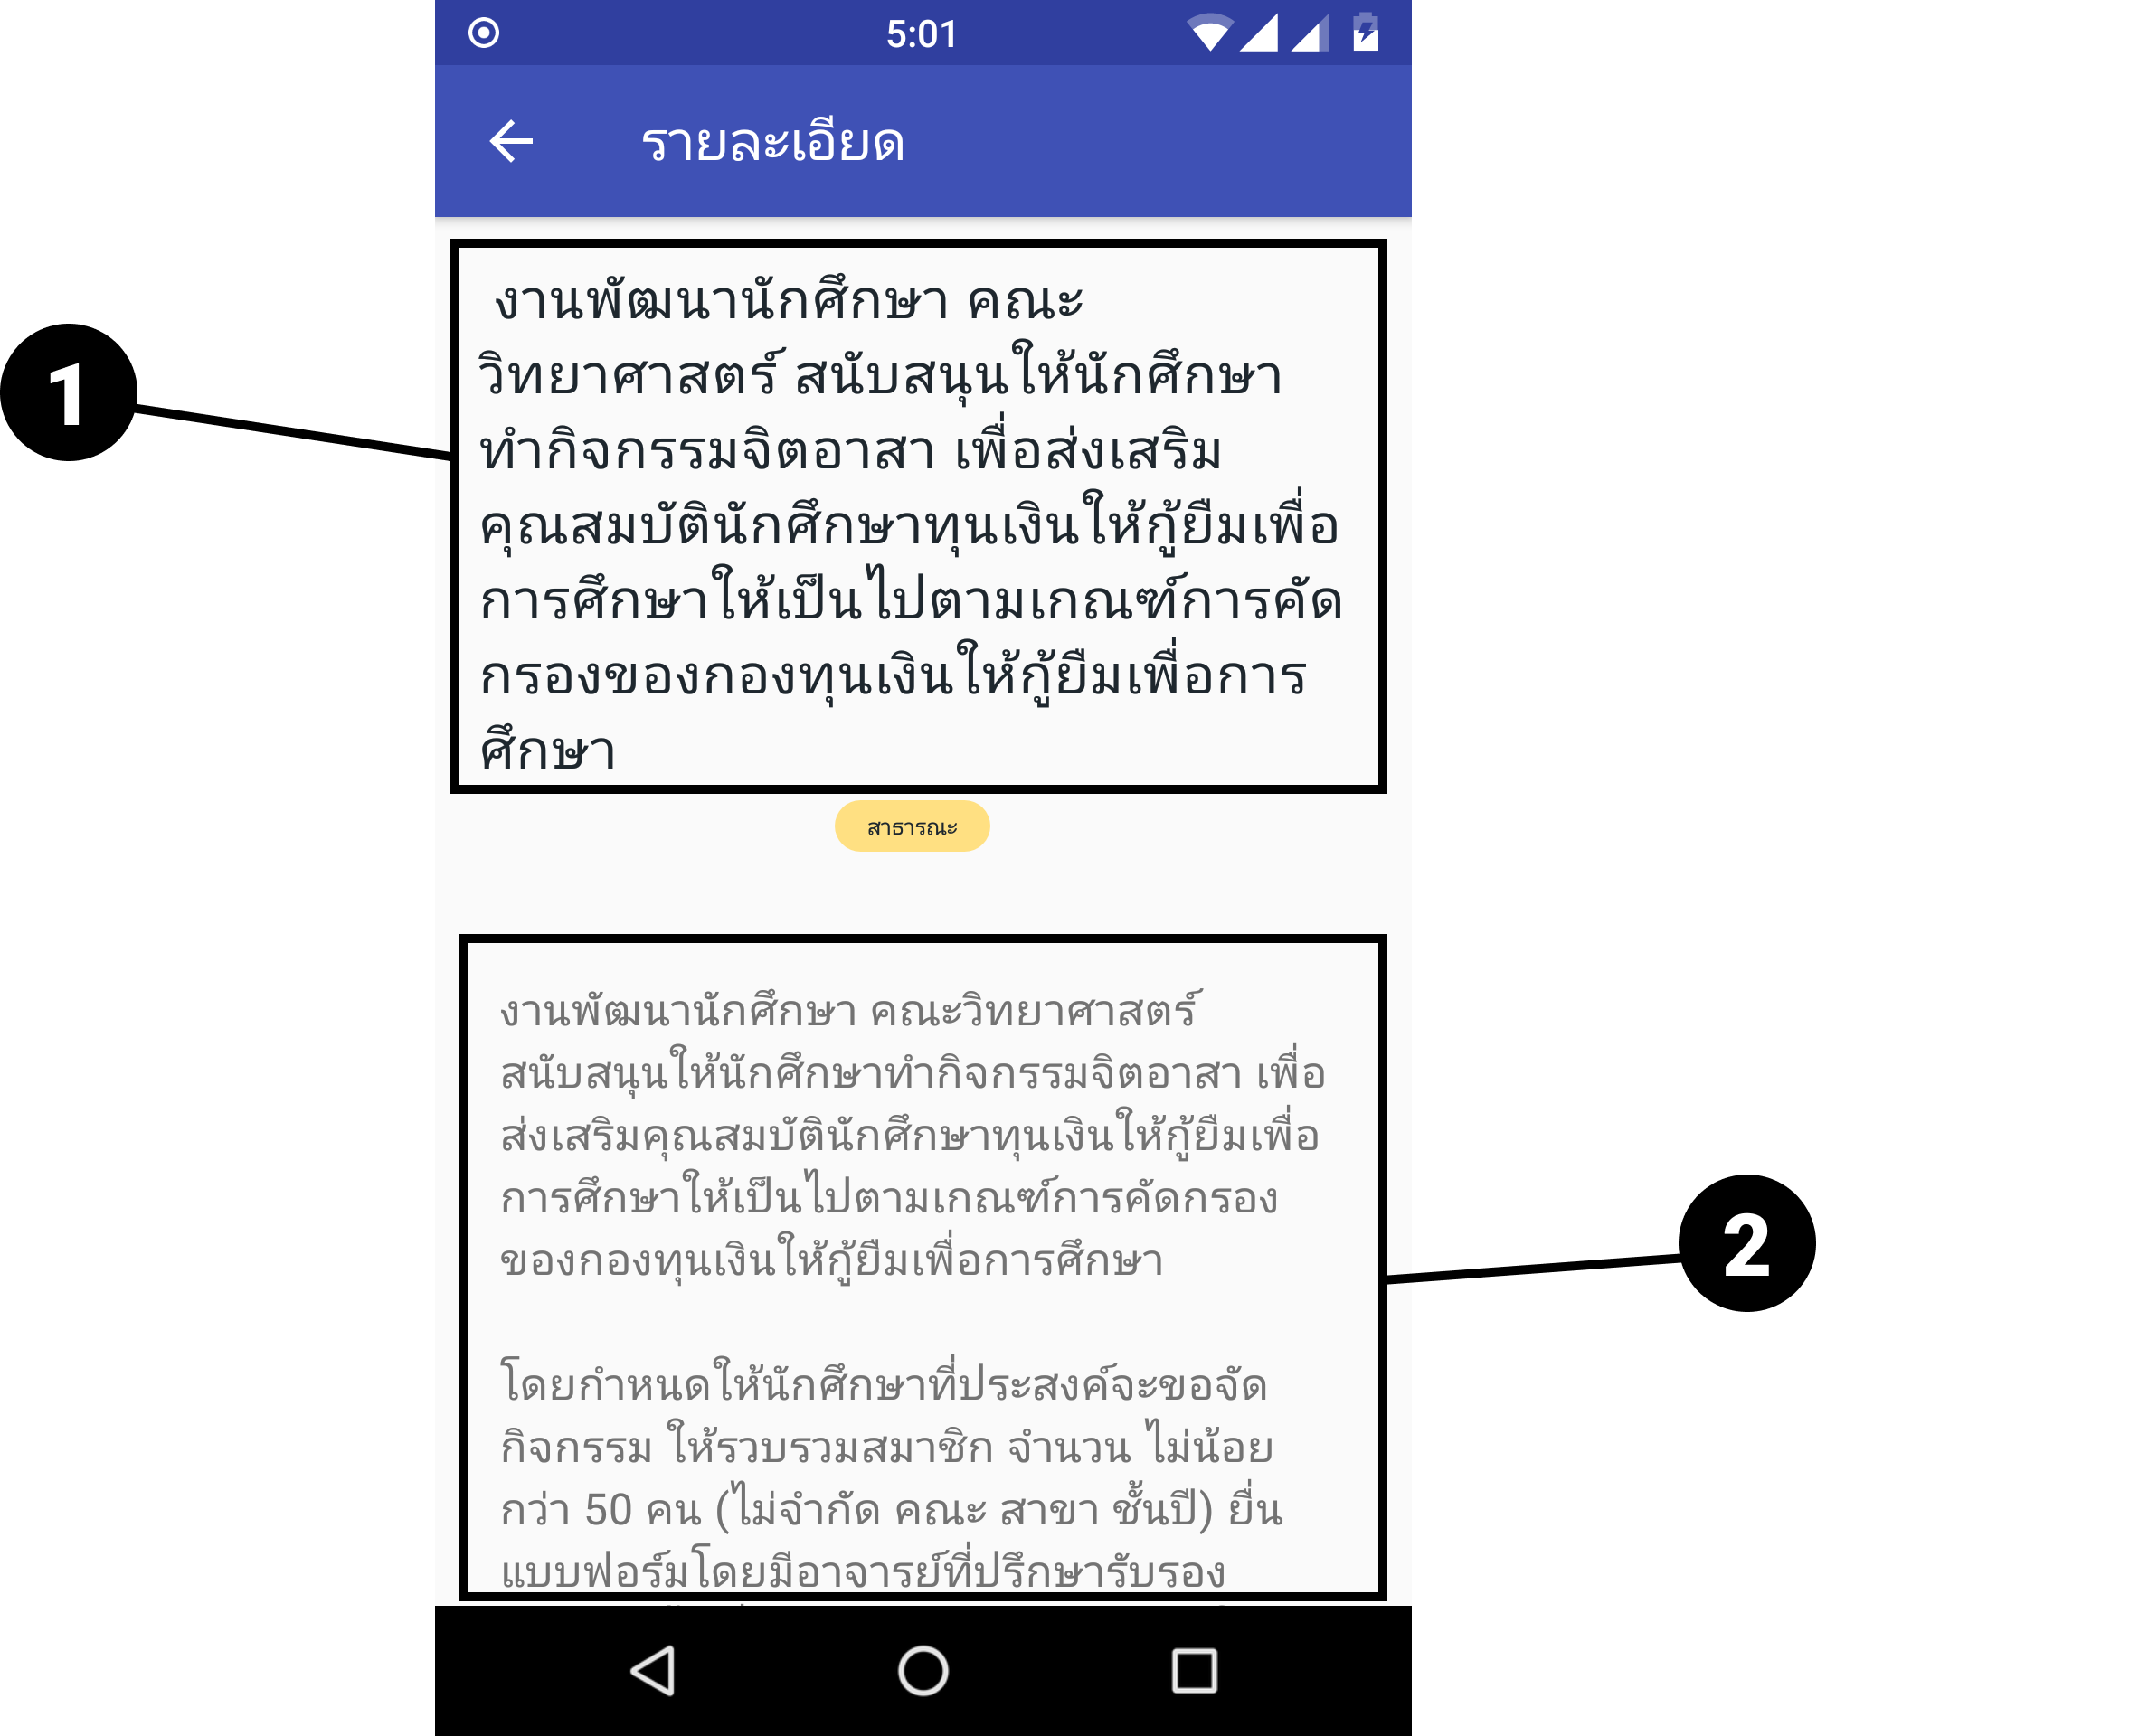
\includegraphics[width=0.5\columnwidth]{Figures/7/Manual/viewpost}
				\caption{หน้ารายละเอียดของข่าวสาร}
				\label{Fig:viewpost}
			\end{figure}
			จากรูปที่ \ref{Fig:viewpost} สามารถอธิบายการใช้งานได้ดังนี้
			\begin{itemize}[label={--}]
				\item หมายเลข 1 คือ หัวข้อข่าวสาร
				\item หมายเลข 1 คือ รายละเอียดของข่าวสาร
			\end{itemize}
		
			\item เมื่อผู้ใช้กดเลือกเมนู Drawer ระบบจะแสดงเมนูนำทางหลักของแอปพลิเคชันซึ่งประกอบไปด้วยเมนู ประชาสัมพันธ์ ข้อความ กำหนดการ เอกสาร ส่งเอกสาร จองคิว คำถามที่พบบ่อย เกี่ยวกับเรา บัญชีผู้ใช้และออกจากระบบ ดังแสดงในรูปที่ \ref{Fig:nav}
			\begin{figure}[H]
				\centering
				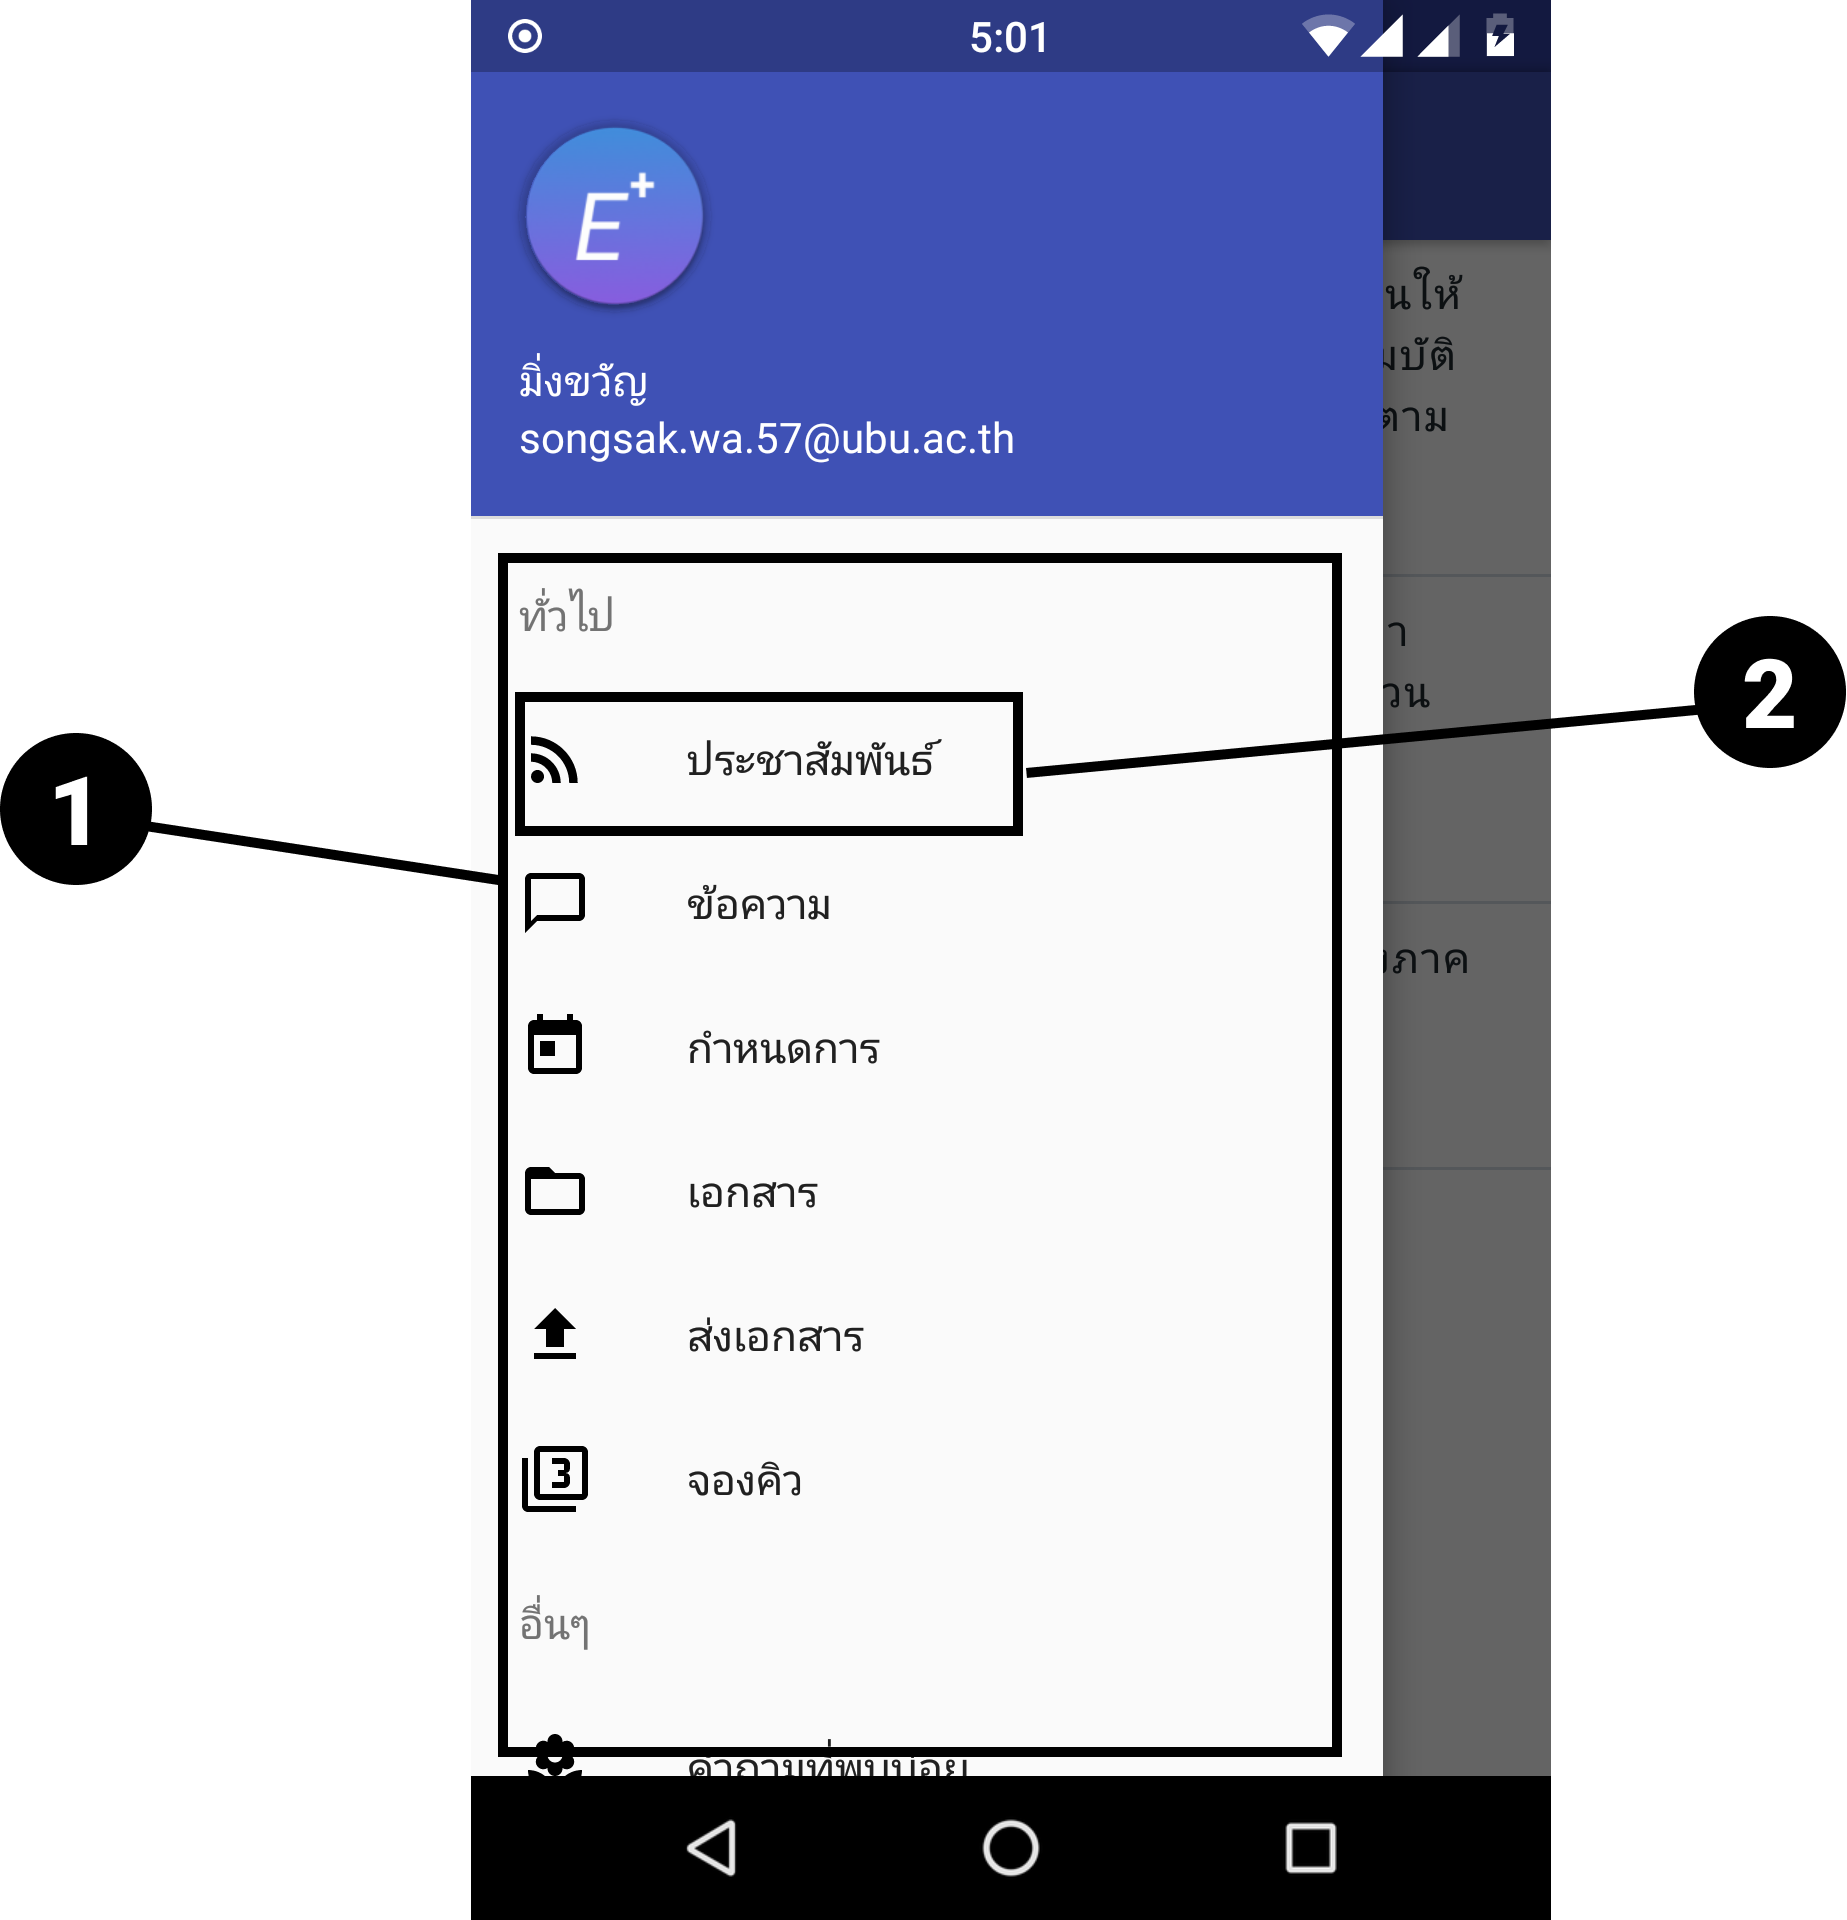
\includegraphics[width=0.5\columnwidth]{Figures/7/Manual/nav}
				\caption{เมนูนำทางหลักของแอปพลิเคชัน}
				\label{Fig:nav}
			\end{figure}
			จากรูปที่ \ref{Fig:nav} สามารถอธิบายการใช้งานได้ดังนี้
			\begin{itemize}[label={--}]
				\item หมายเลข 1 คือ รายการเมนูนำทางหลักของแอปพลิเคชัน
				\item หมายเลข 2 คือ เมนูนำทาง
			\end{itemize}
		
			\item เมื่อผู้ใช้เลือกเมนูกำหนดการ ระบบจะแสดงหน้าจอกำหนดการ ดังแสดงในรูปที่ \ref{Fig:event}
			\begin{figure}[H]
				\centering
				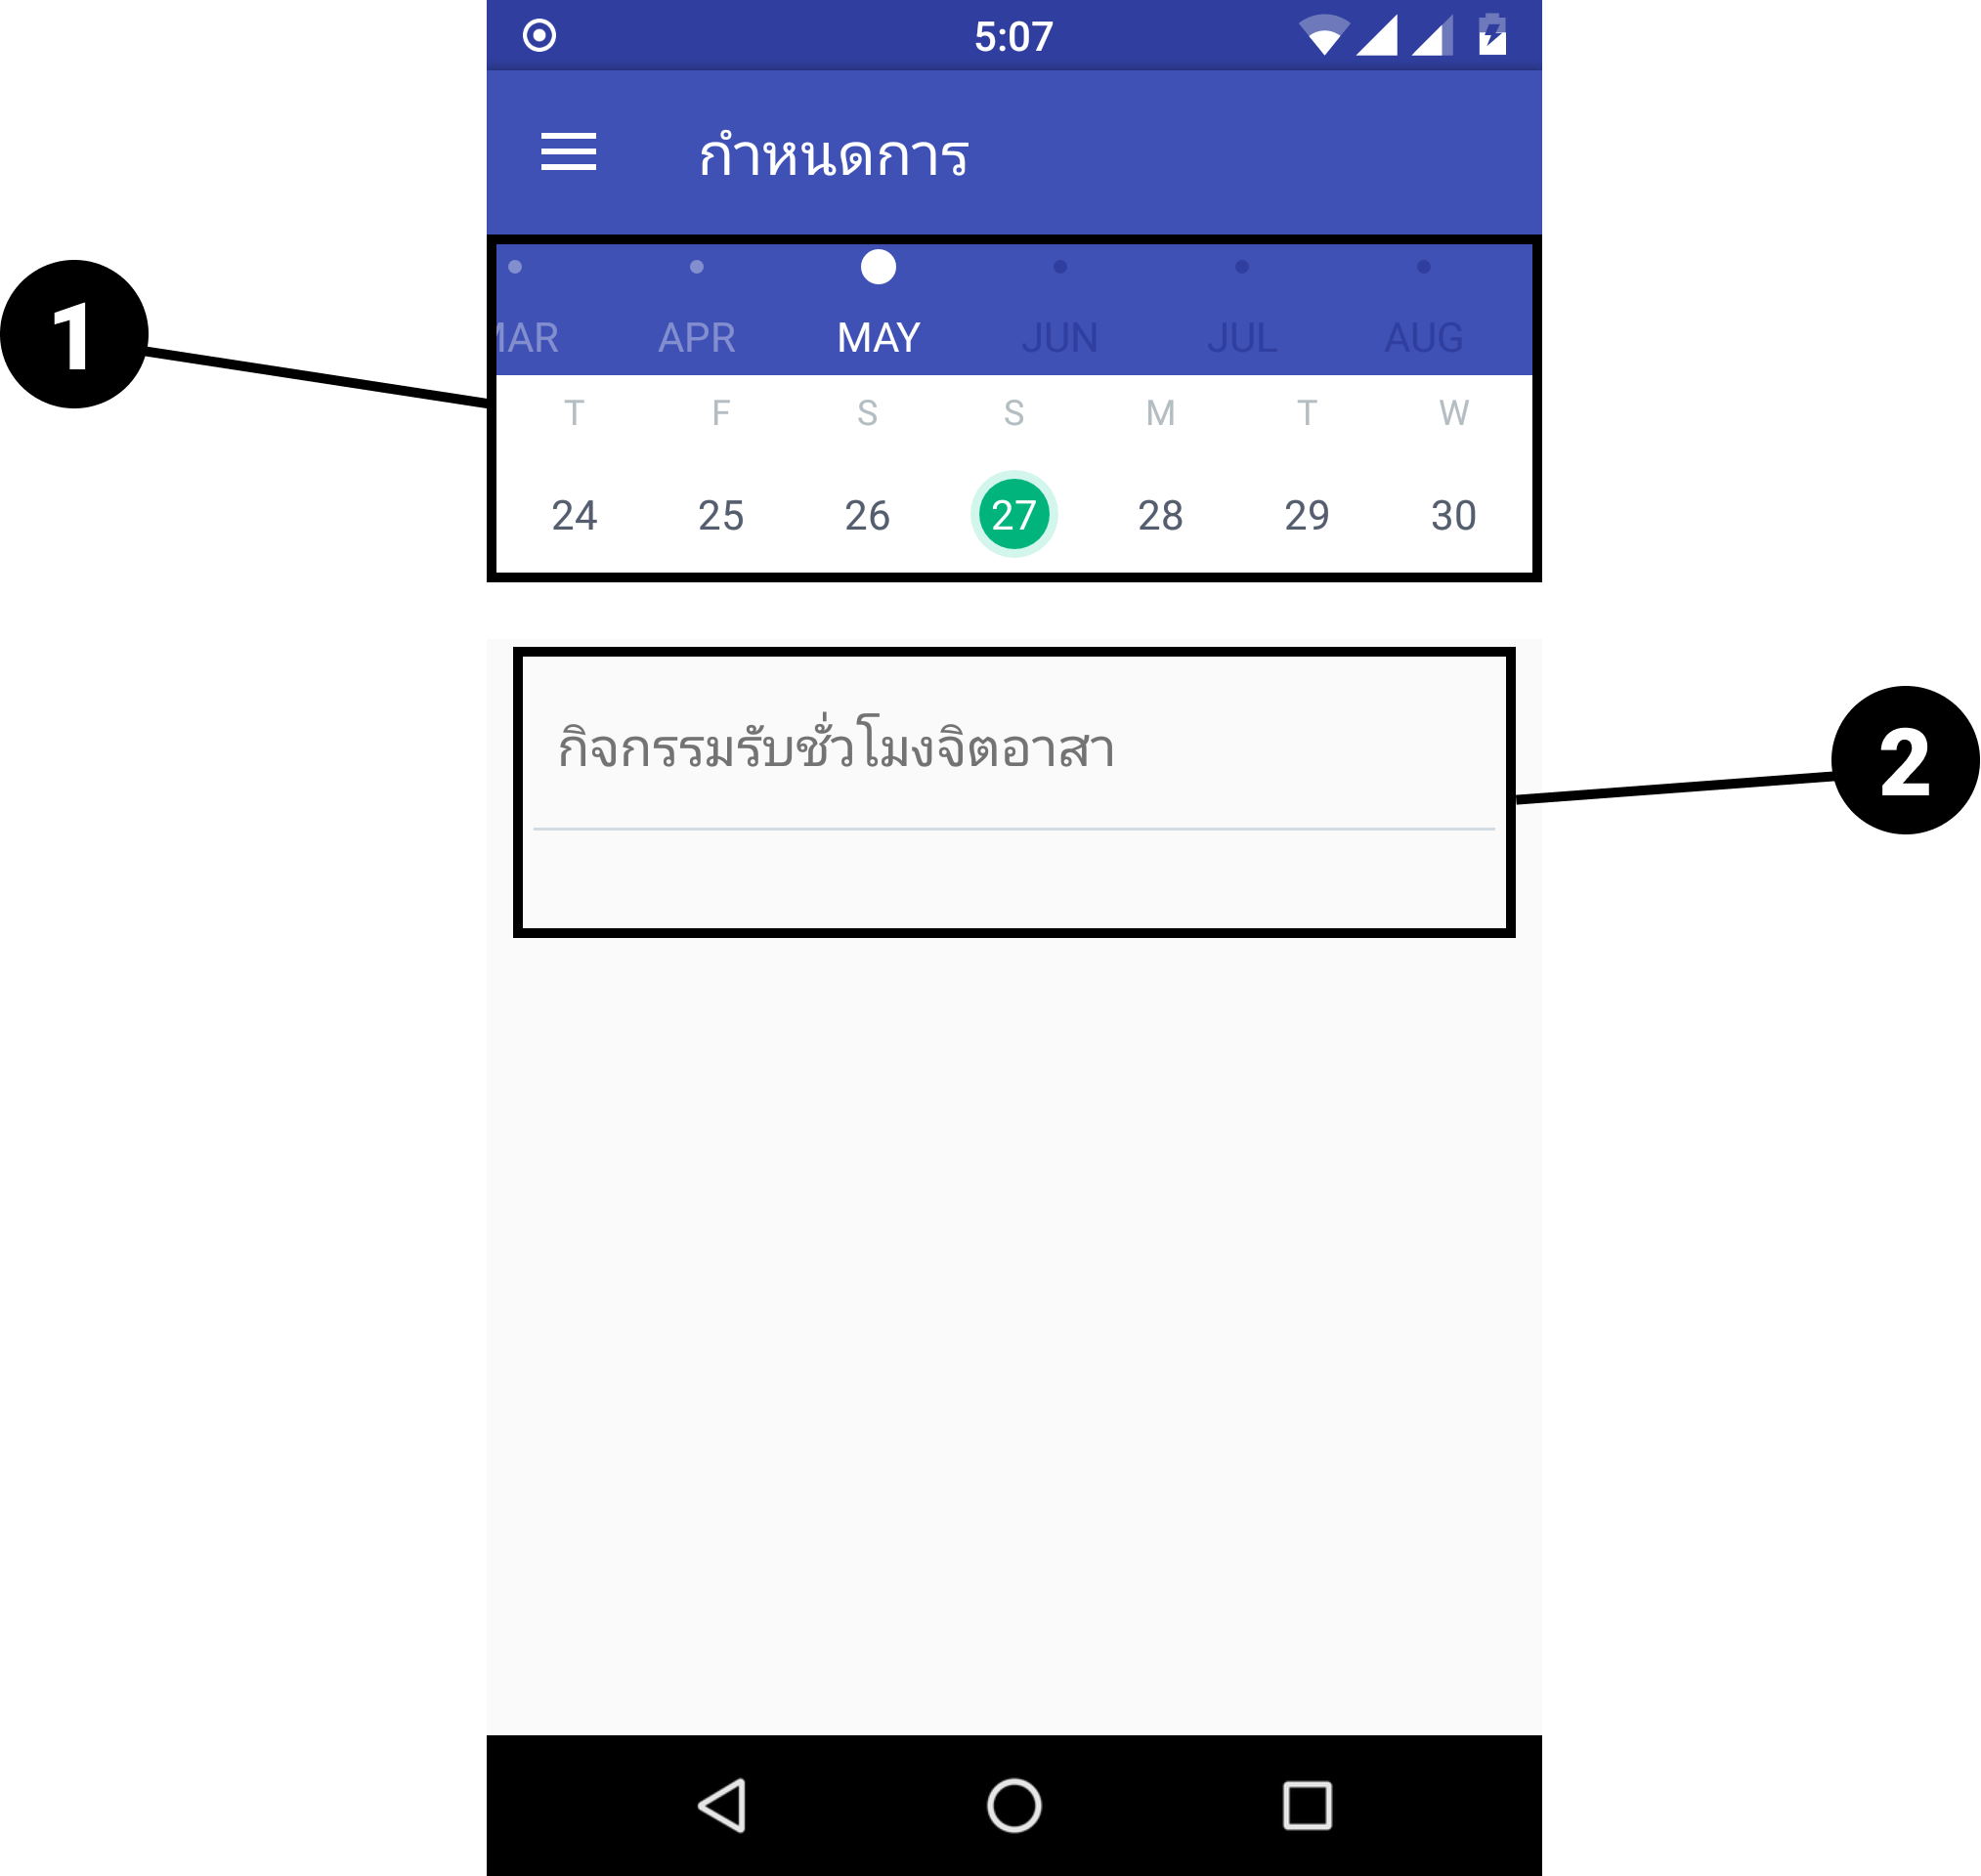
\includegraphics[width=0.5\columnwidth]{Figures/7/Manual/event}
				\caption{หน้าจอกำหนดการ}
				\label{Fig:event}
			\end{figure}	\item ส่วนของหน้าเมนูแอปพลิเคชันสำหรับนักศึกษา

		\item หน้าจอต้อนรับแสดงผลทุกครั้งเมื่อผู้ใช้ทำการเปิดใช้งานแอปพลิเคชัน ดังแสดงในรูปที่ \ref{Fig:open}
		\begin{figure}[H]
			\centering
			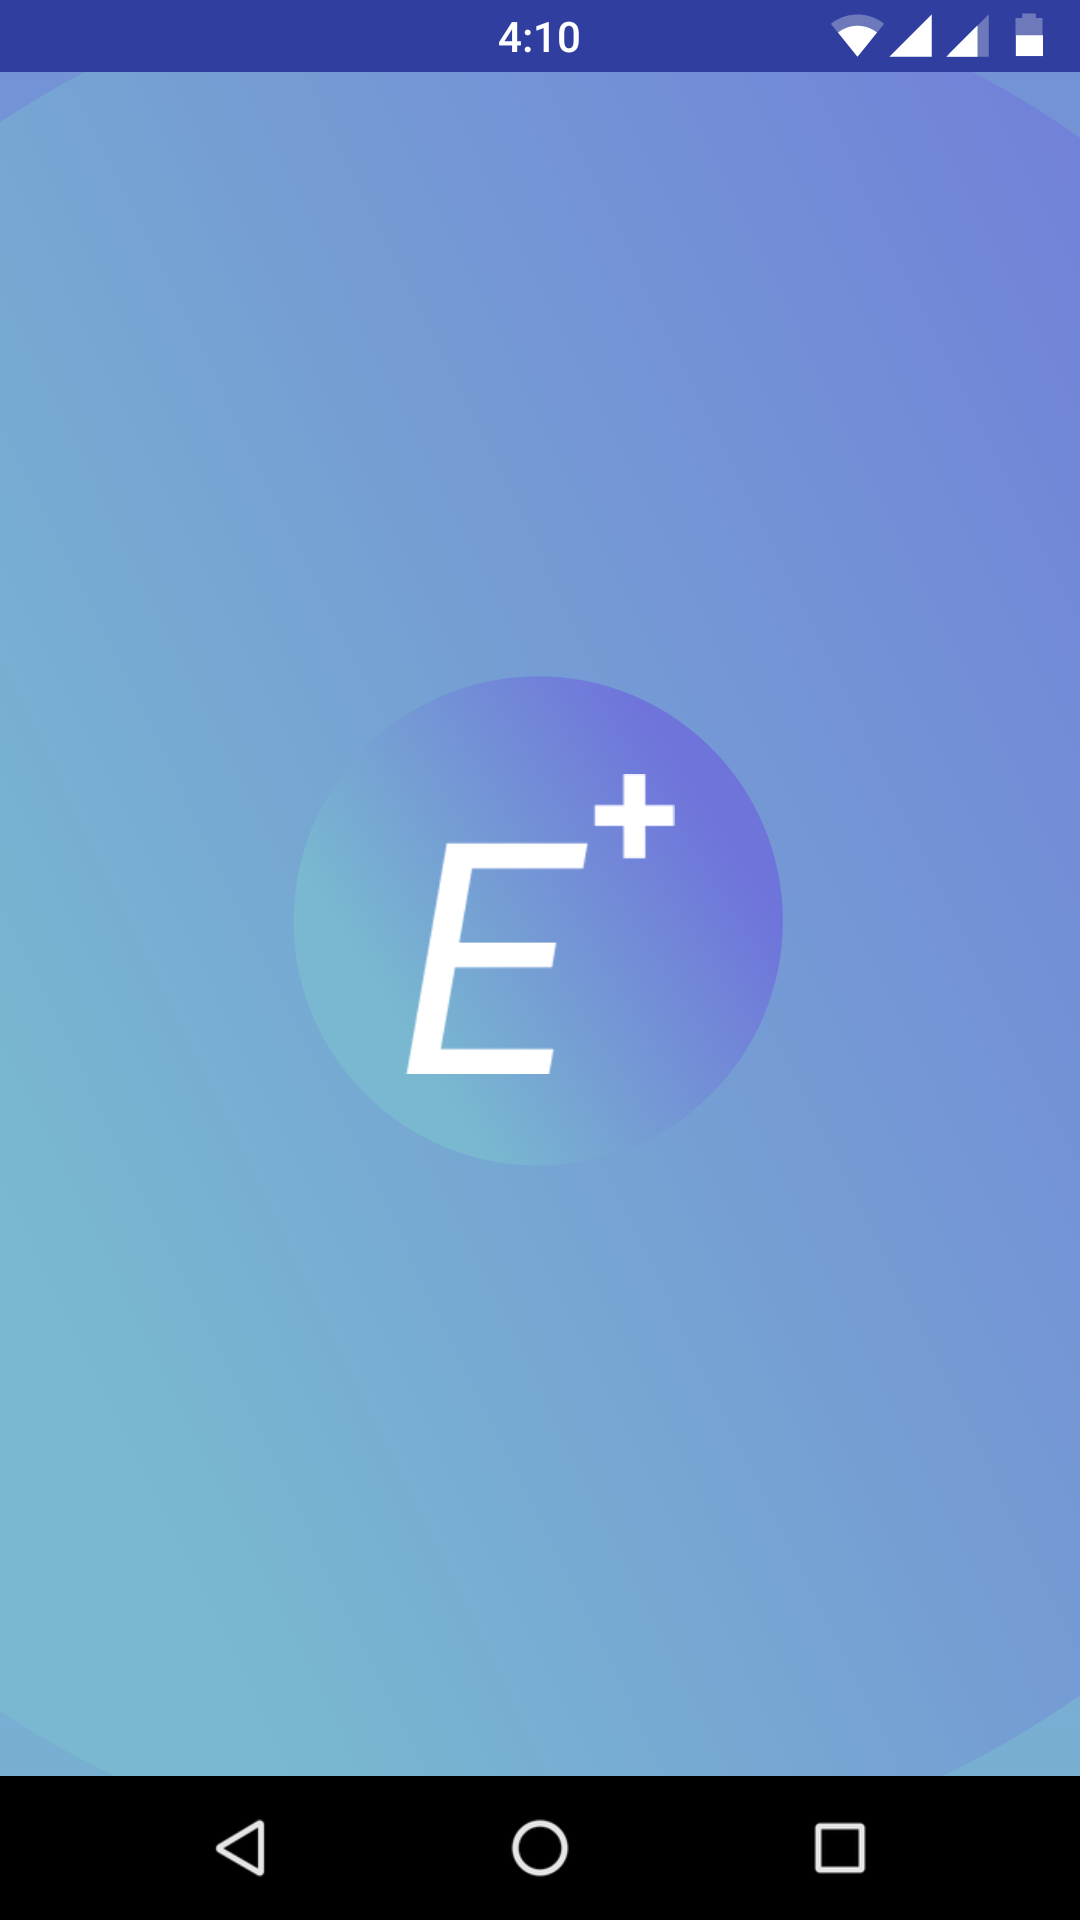
\includegraphics[width=0.3\columnwidth]{Figures/7/Manual/open}
			\caption{หน้าจอต้อนรับ}
			\label{Fig:open}
		\end{figure}
		
		\item เมื่อระบบทำการตรวจสอบว่ามีสิทธิ์(Permission)ในการใช้งานแอปพลิเคชันที่ผู้ใช้ยังไม่ได้อนุญาตให้เข้าถึง ระบบจะแสดงหน้าต่างขอสิทธิ์การเข้าถึง ดังแสดงในรูปที่ \ref{Fig:permission}
		\begin{figure}[H]
			\centering
			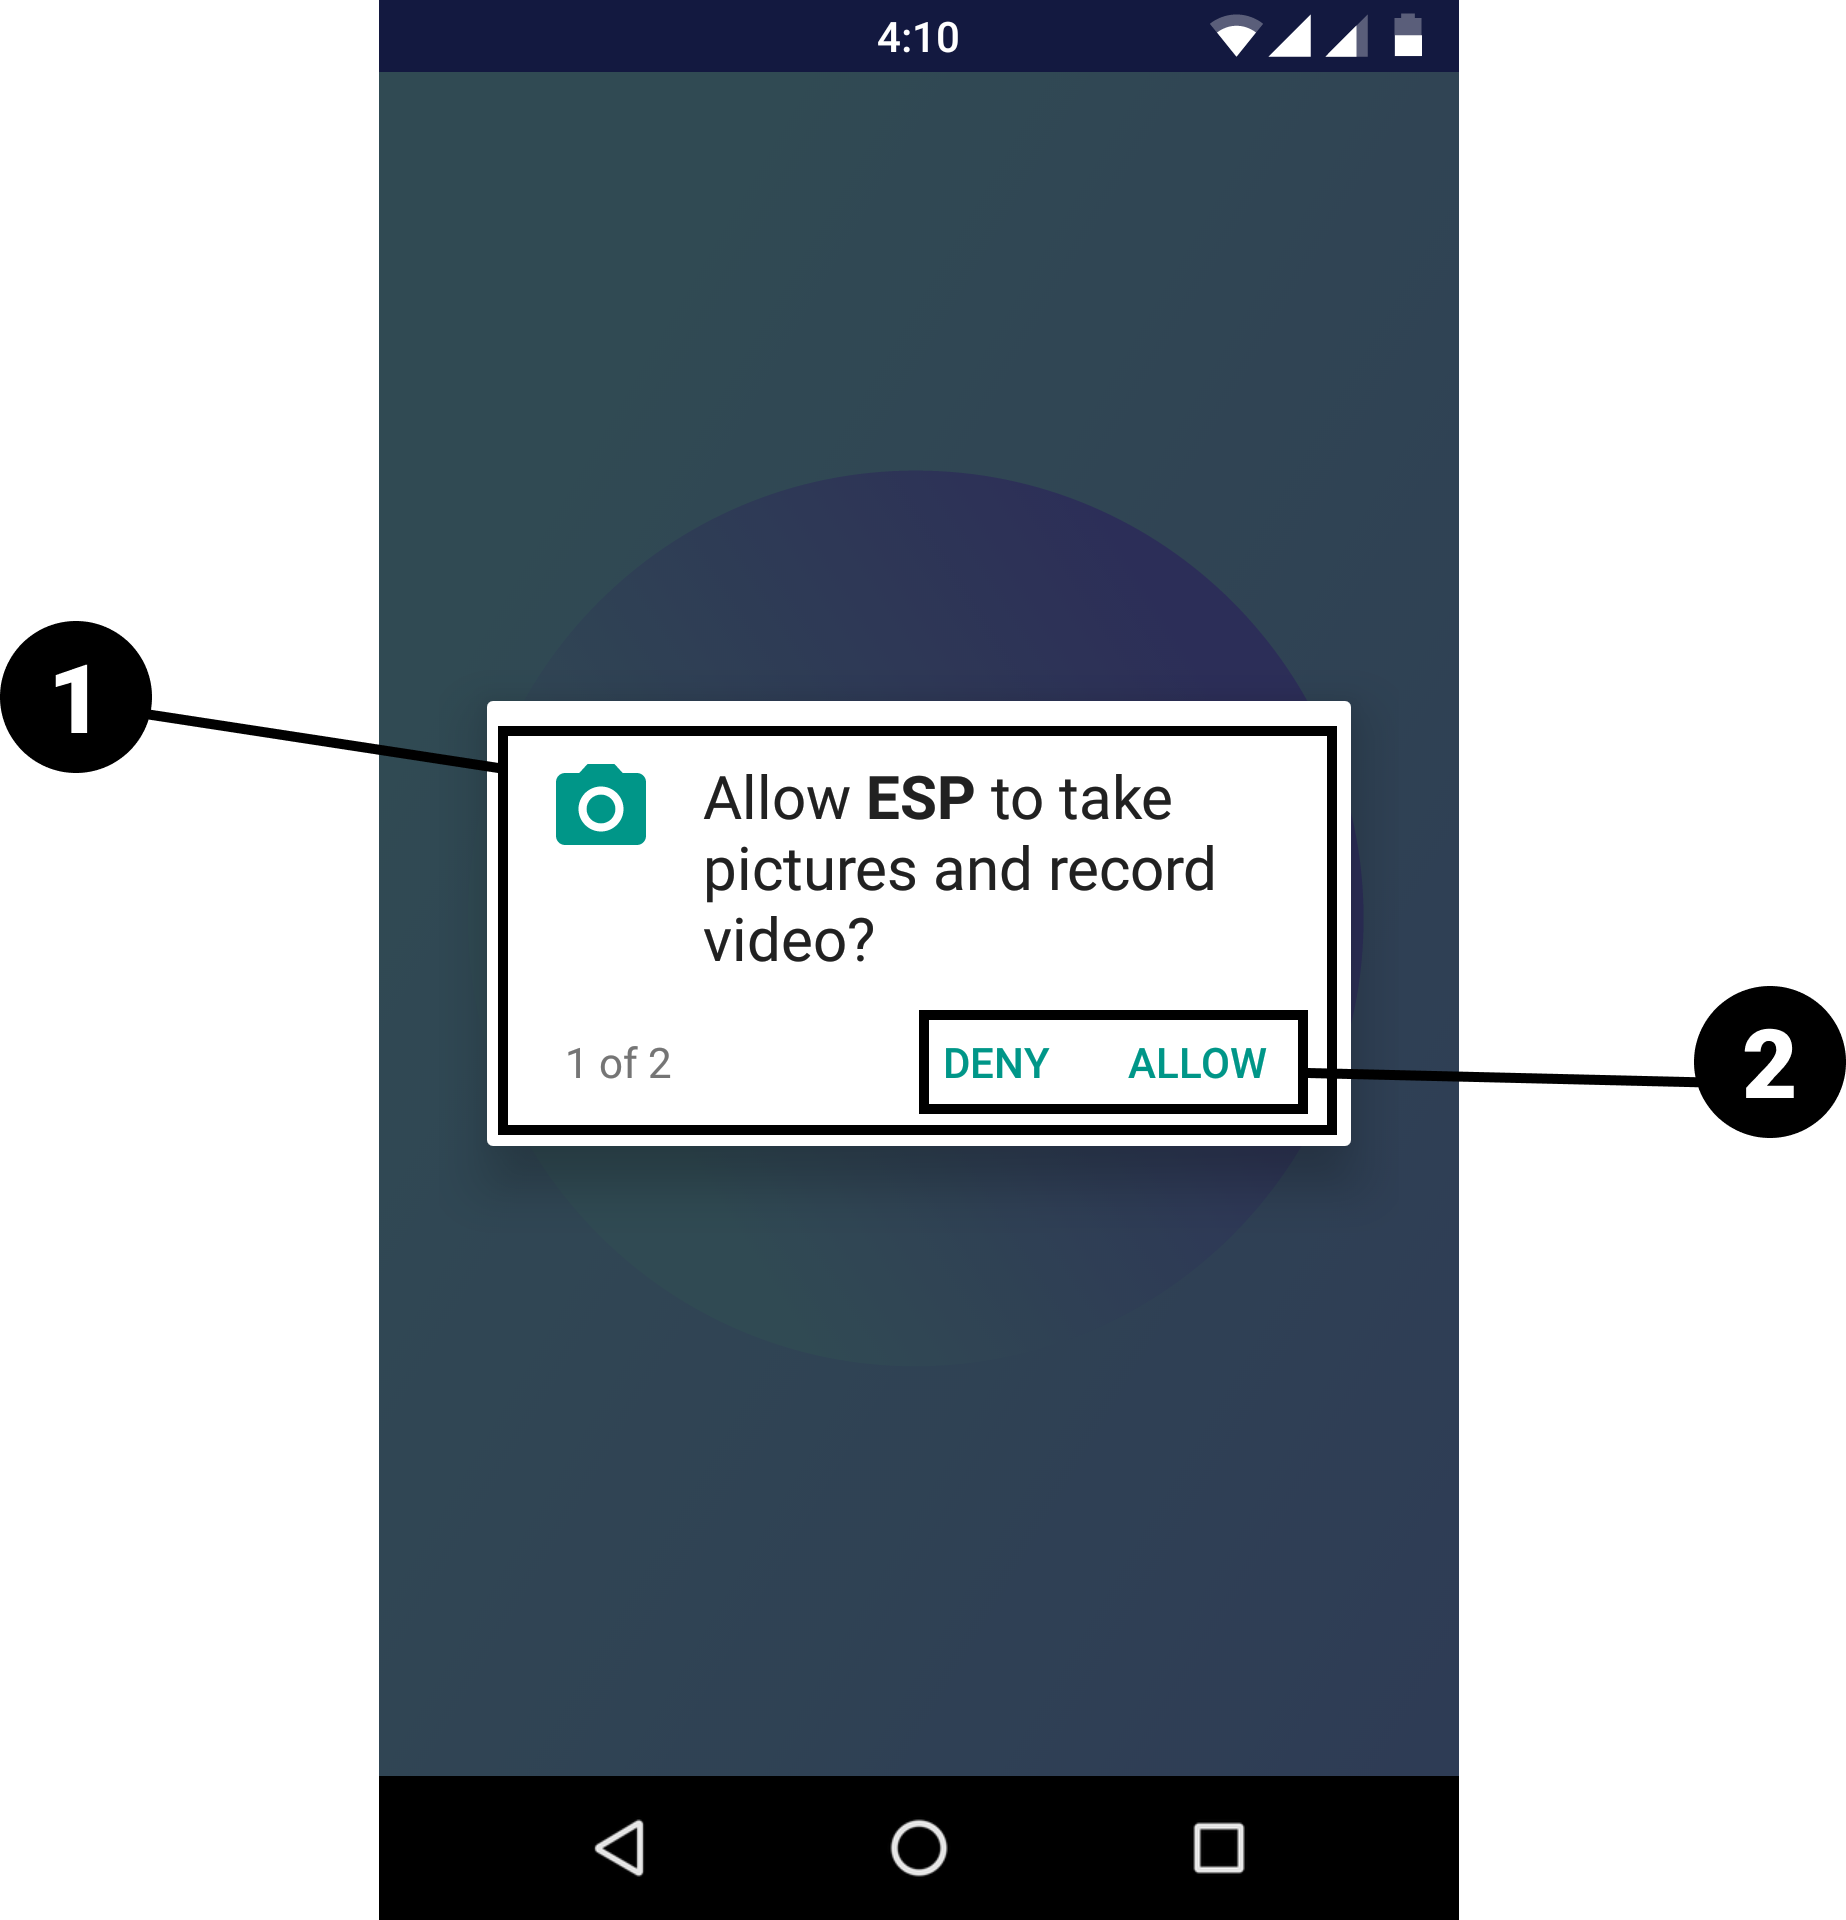
\includegraphics[width=0.5\columnwidth]{Figures/7/Manual/permission}
			\caption{หน้าต่างขอสิทธิ์การเข้าถึง}
			\label{Fig:permission}
		\end{figure}
		จากรูปที่ \ref{Fig:permission} สามารถอธิบายการใช้งานได้ดังนี้
		\begin{itemize}[label={--}]
			\item หมายเลข 1 คือ หน้าต่างขอสิทธิ์การเข้าถึงข้อมูล
			\item หมายเลข 2 คือ ปุ่มให้สิทธิ์และยกเลิกการให้สิทธิ์
		\end{itemize}
	
			\begin{figure}[H]
				\centering
				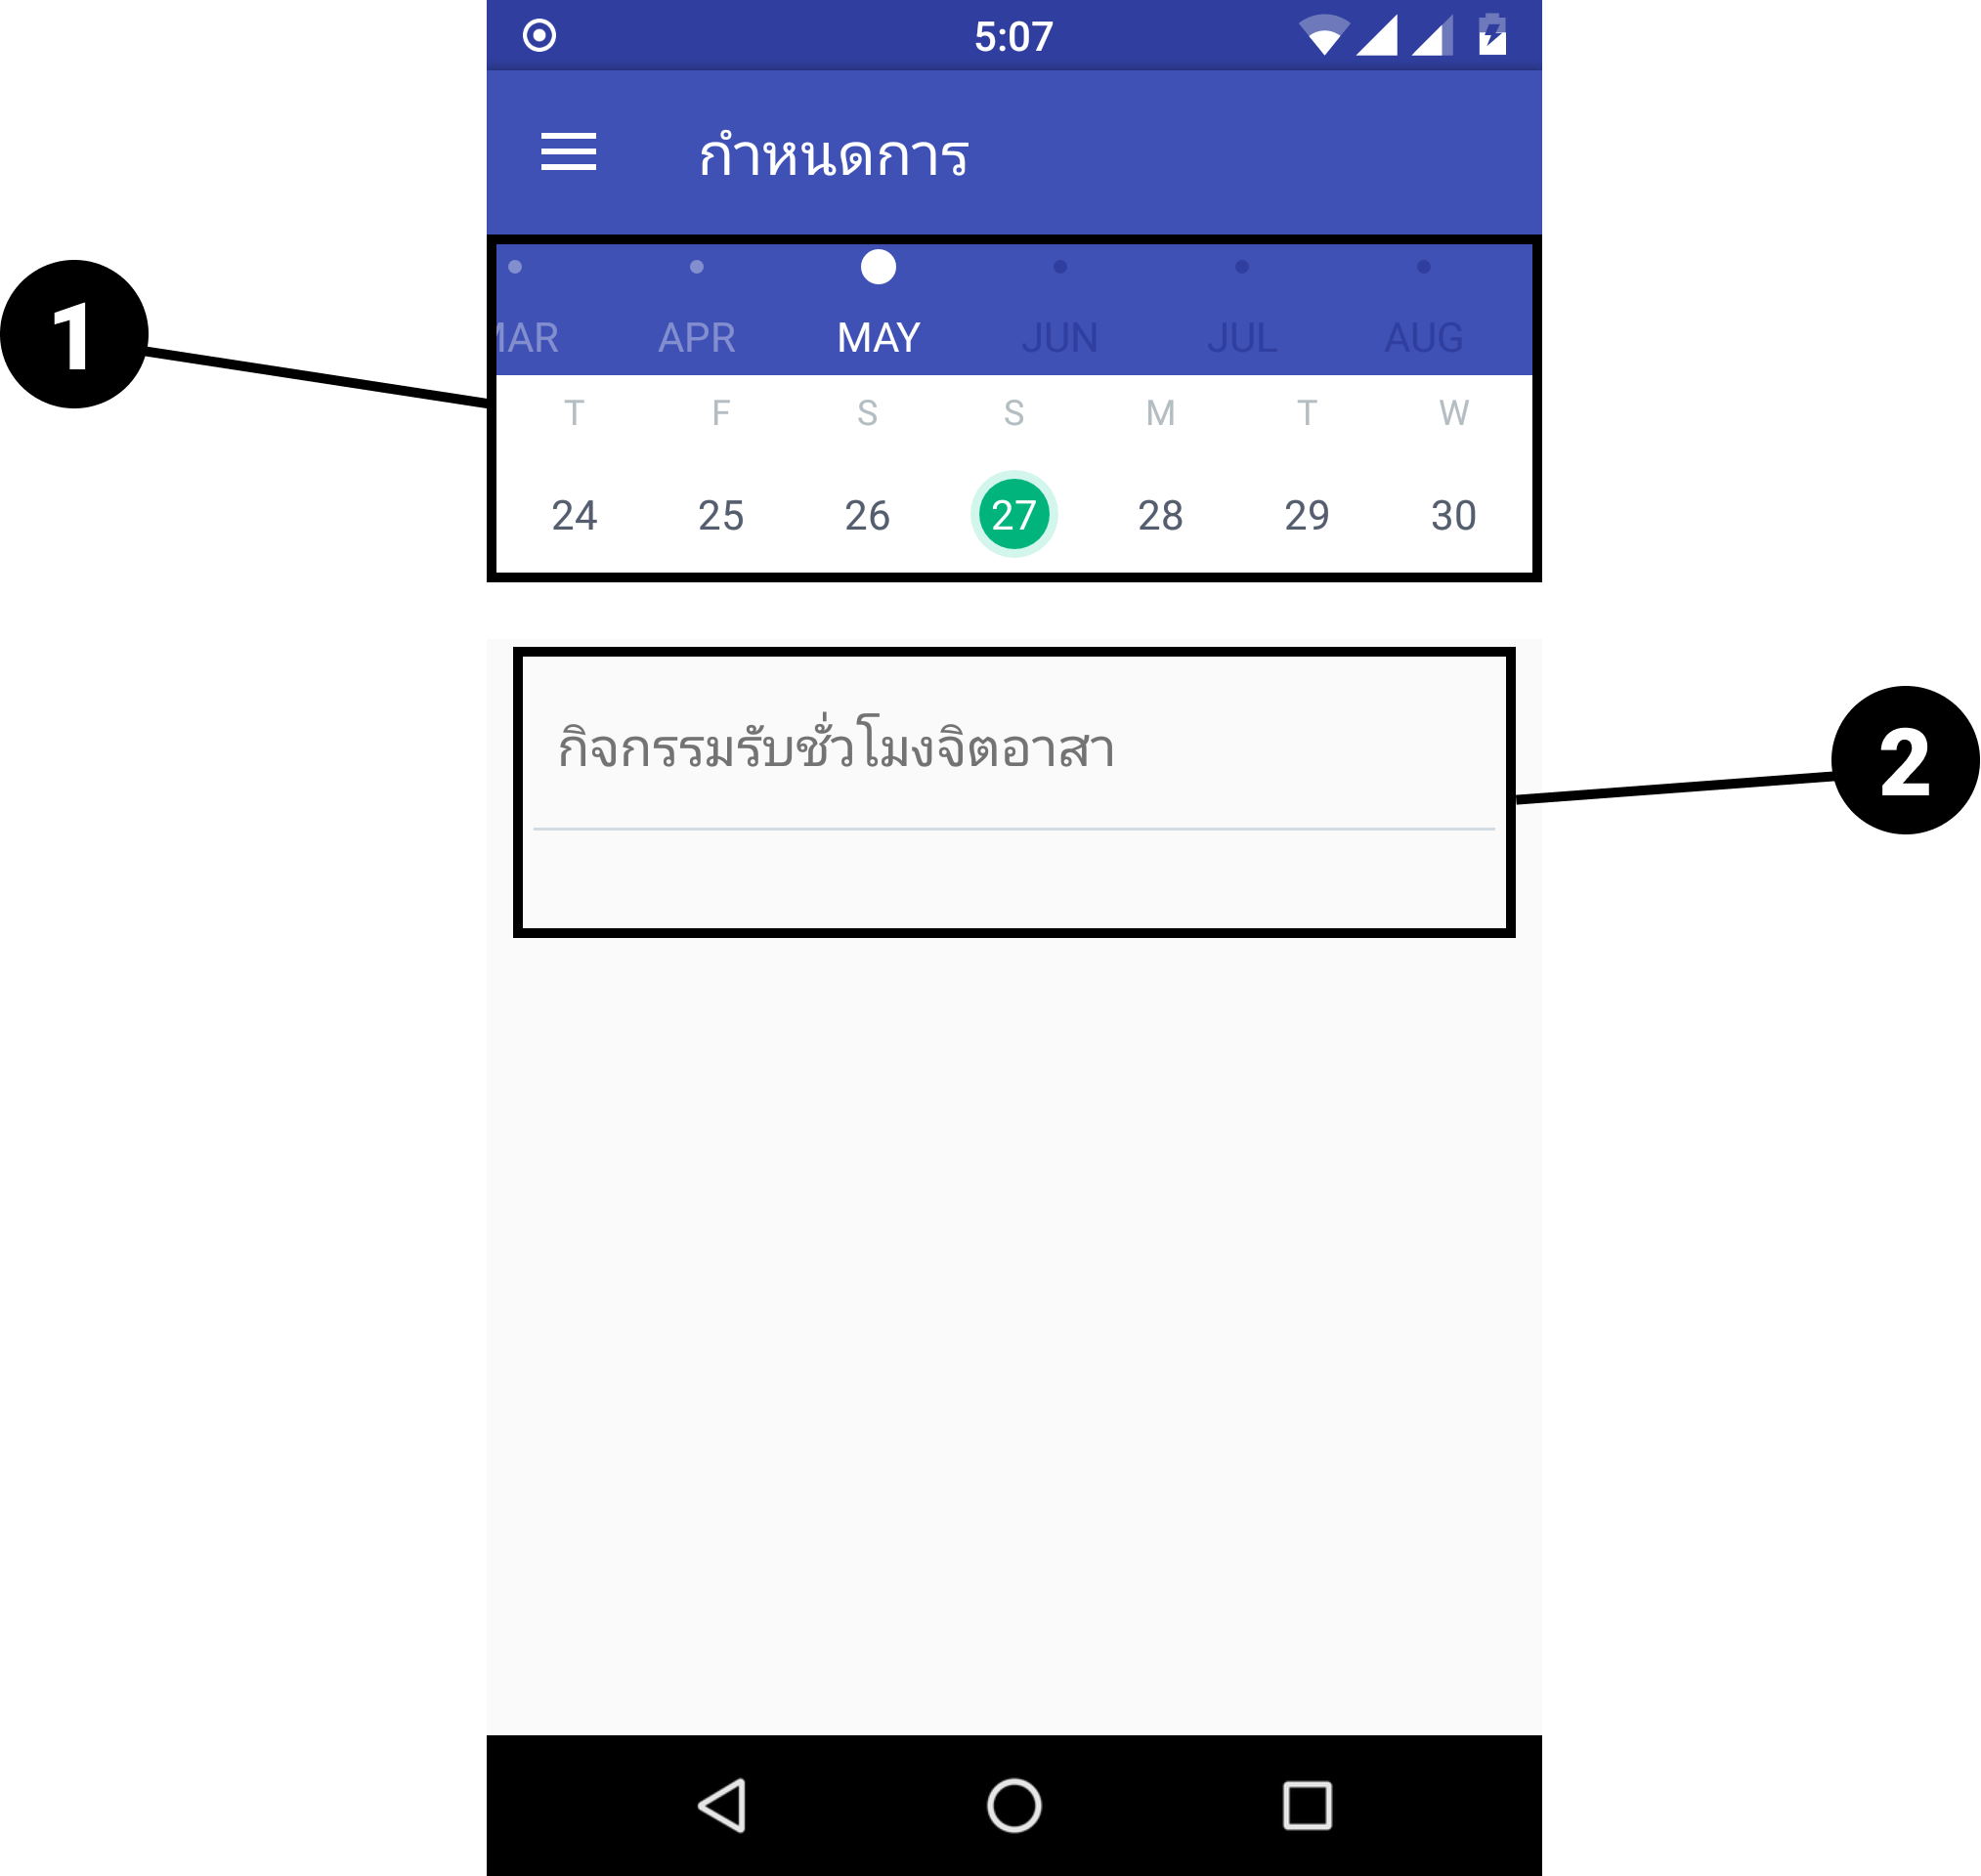
\includegraphics[width=0.5\columnwidth]{Figures/7/Manual/event}
				\caption{หน้าแสดงกำหนดการ}
				\label{Fig:event}
			\end{figure}
			จากรูปที่ \ref{Fig:event} สามารถอธิบายการใช้งานได้ดังนี้
			\begin{itemize}[label={--}]
				\item หมายเลข 1 คือ ปฏิทินแสดงวันที่ปัจจุบันและผู้ใช้สามารถเลือกวันที่ต้องการเพื่อดูกำหนดการก่อนหน้า
				\item หมายเลข 2 คือ แสดงรายการกำหนดการของวันนั้น ๆ
			\end{itemize}
				
			\item เมื่อผู้ใช้เลือกเมนูเอกสาร ระบบจะแสดงหน้าจอรายการเอกสาร ดังแสดงในรูปที่ \ref{Fig:doc}
			\begin{figure}[H]
				\centering
				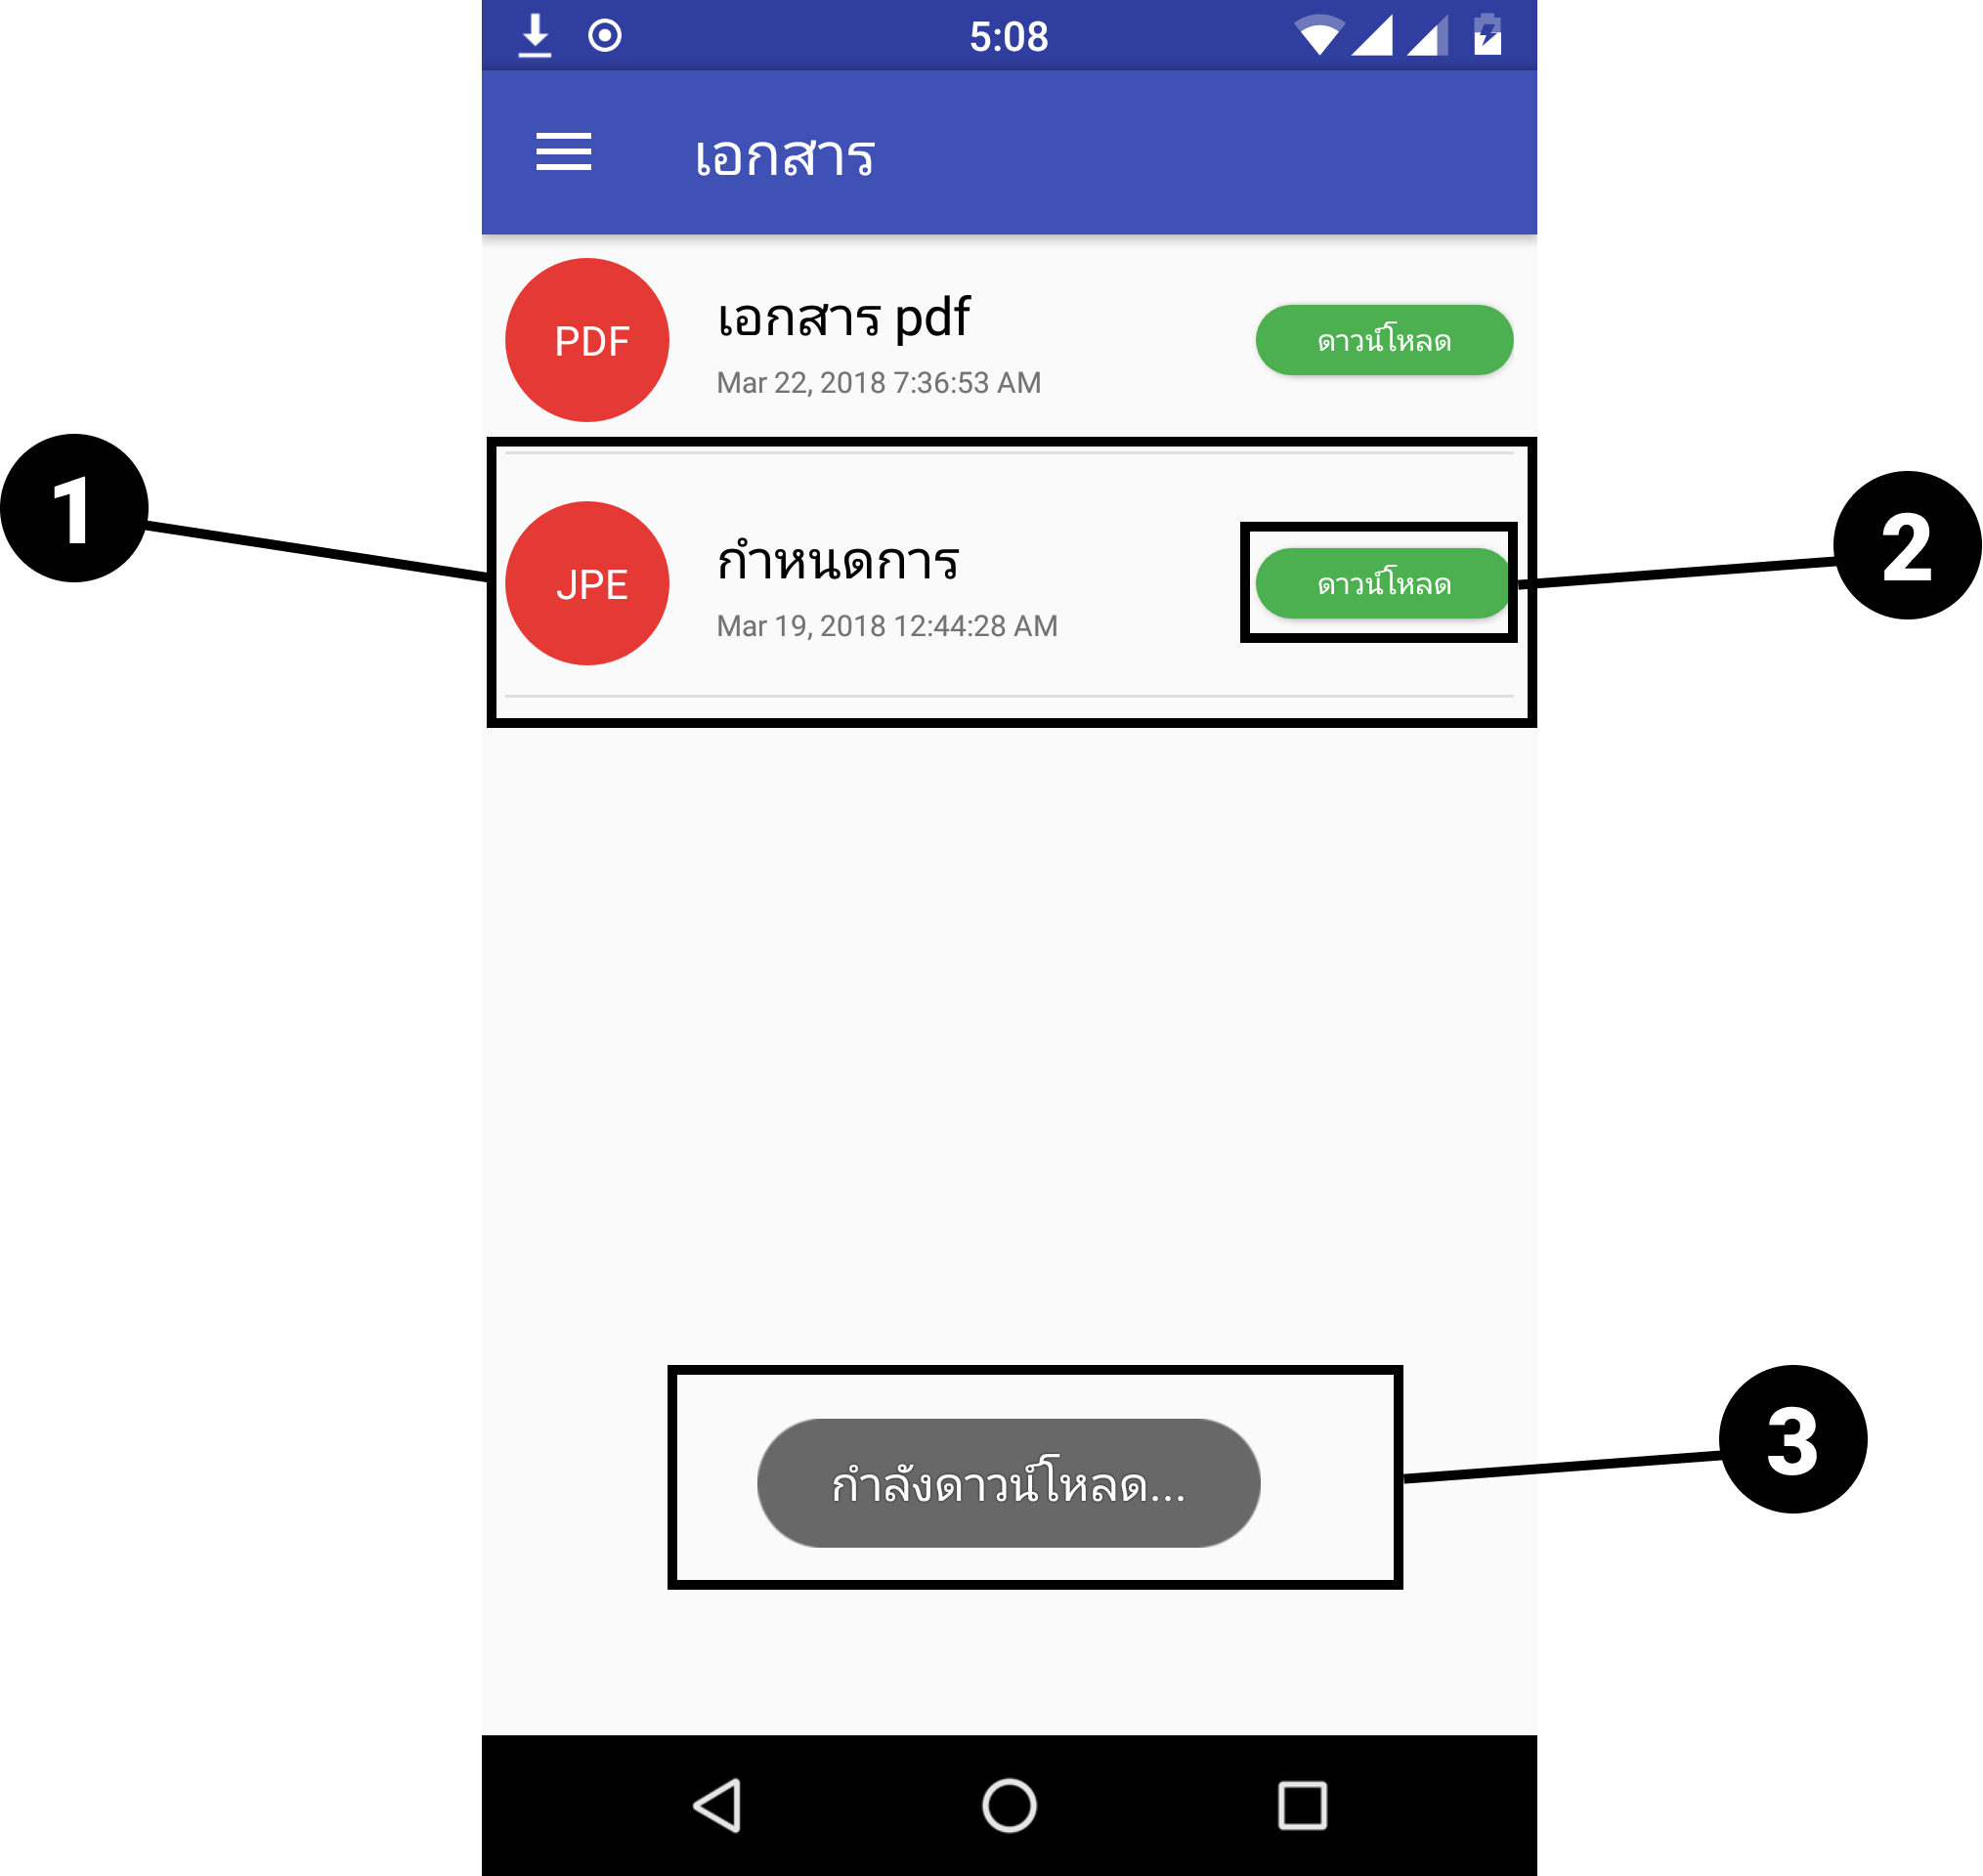
\includegraphics[width=0.5\columnwidth]{Figures/7/Manual/doc}
				\caption{หน้าจอเอกสาร}
				\label{Fig:doc}
			\end{figure}
			จากรูปที่ \ref{Fig:doc} สามารถอธิบายการใช้งานได้ดังนี้
			\begin{itemize}[label={--}]
				\item หมายเลข 1 คือ รายการเอกสาร
				\item หมายเลข 2 คือ ปุ่มดาวน์โหลดเอกสาร
				\item หมายเลข 3 คือ สถานะการดาวน์โหลดเอกสาร
			\end{itemize}
		
			\item เมื่อผู้ใช้เลือกเมนูข้อความ ระบบจะแสดงหน้าจอสนทนา ดังแสดงในรูปที่ \ref{Fig:chat}
			\begin{figure}[H]
				\centering
				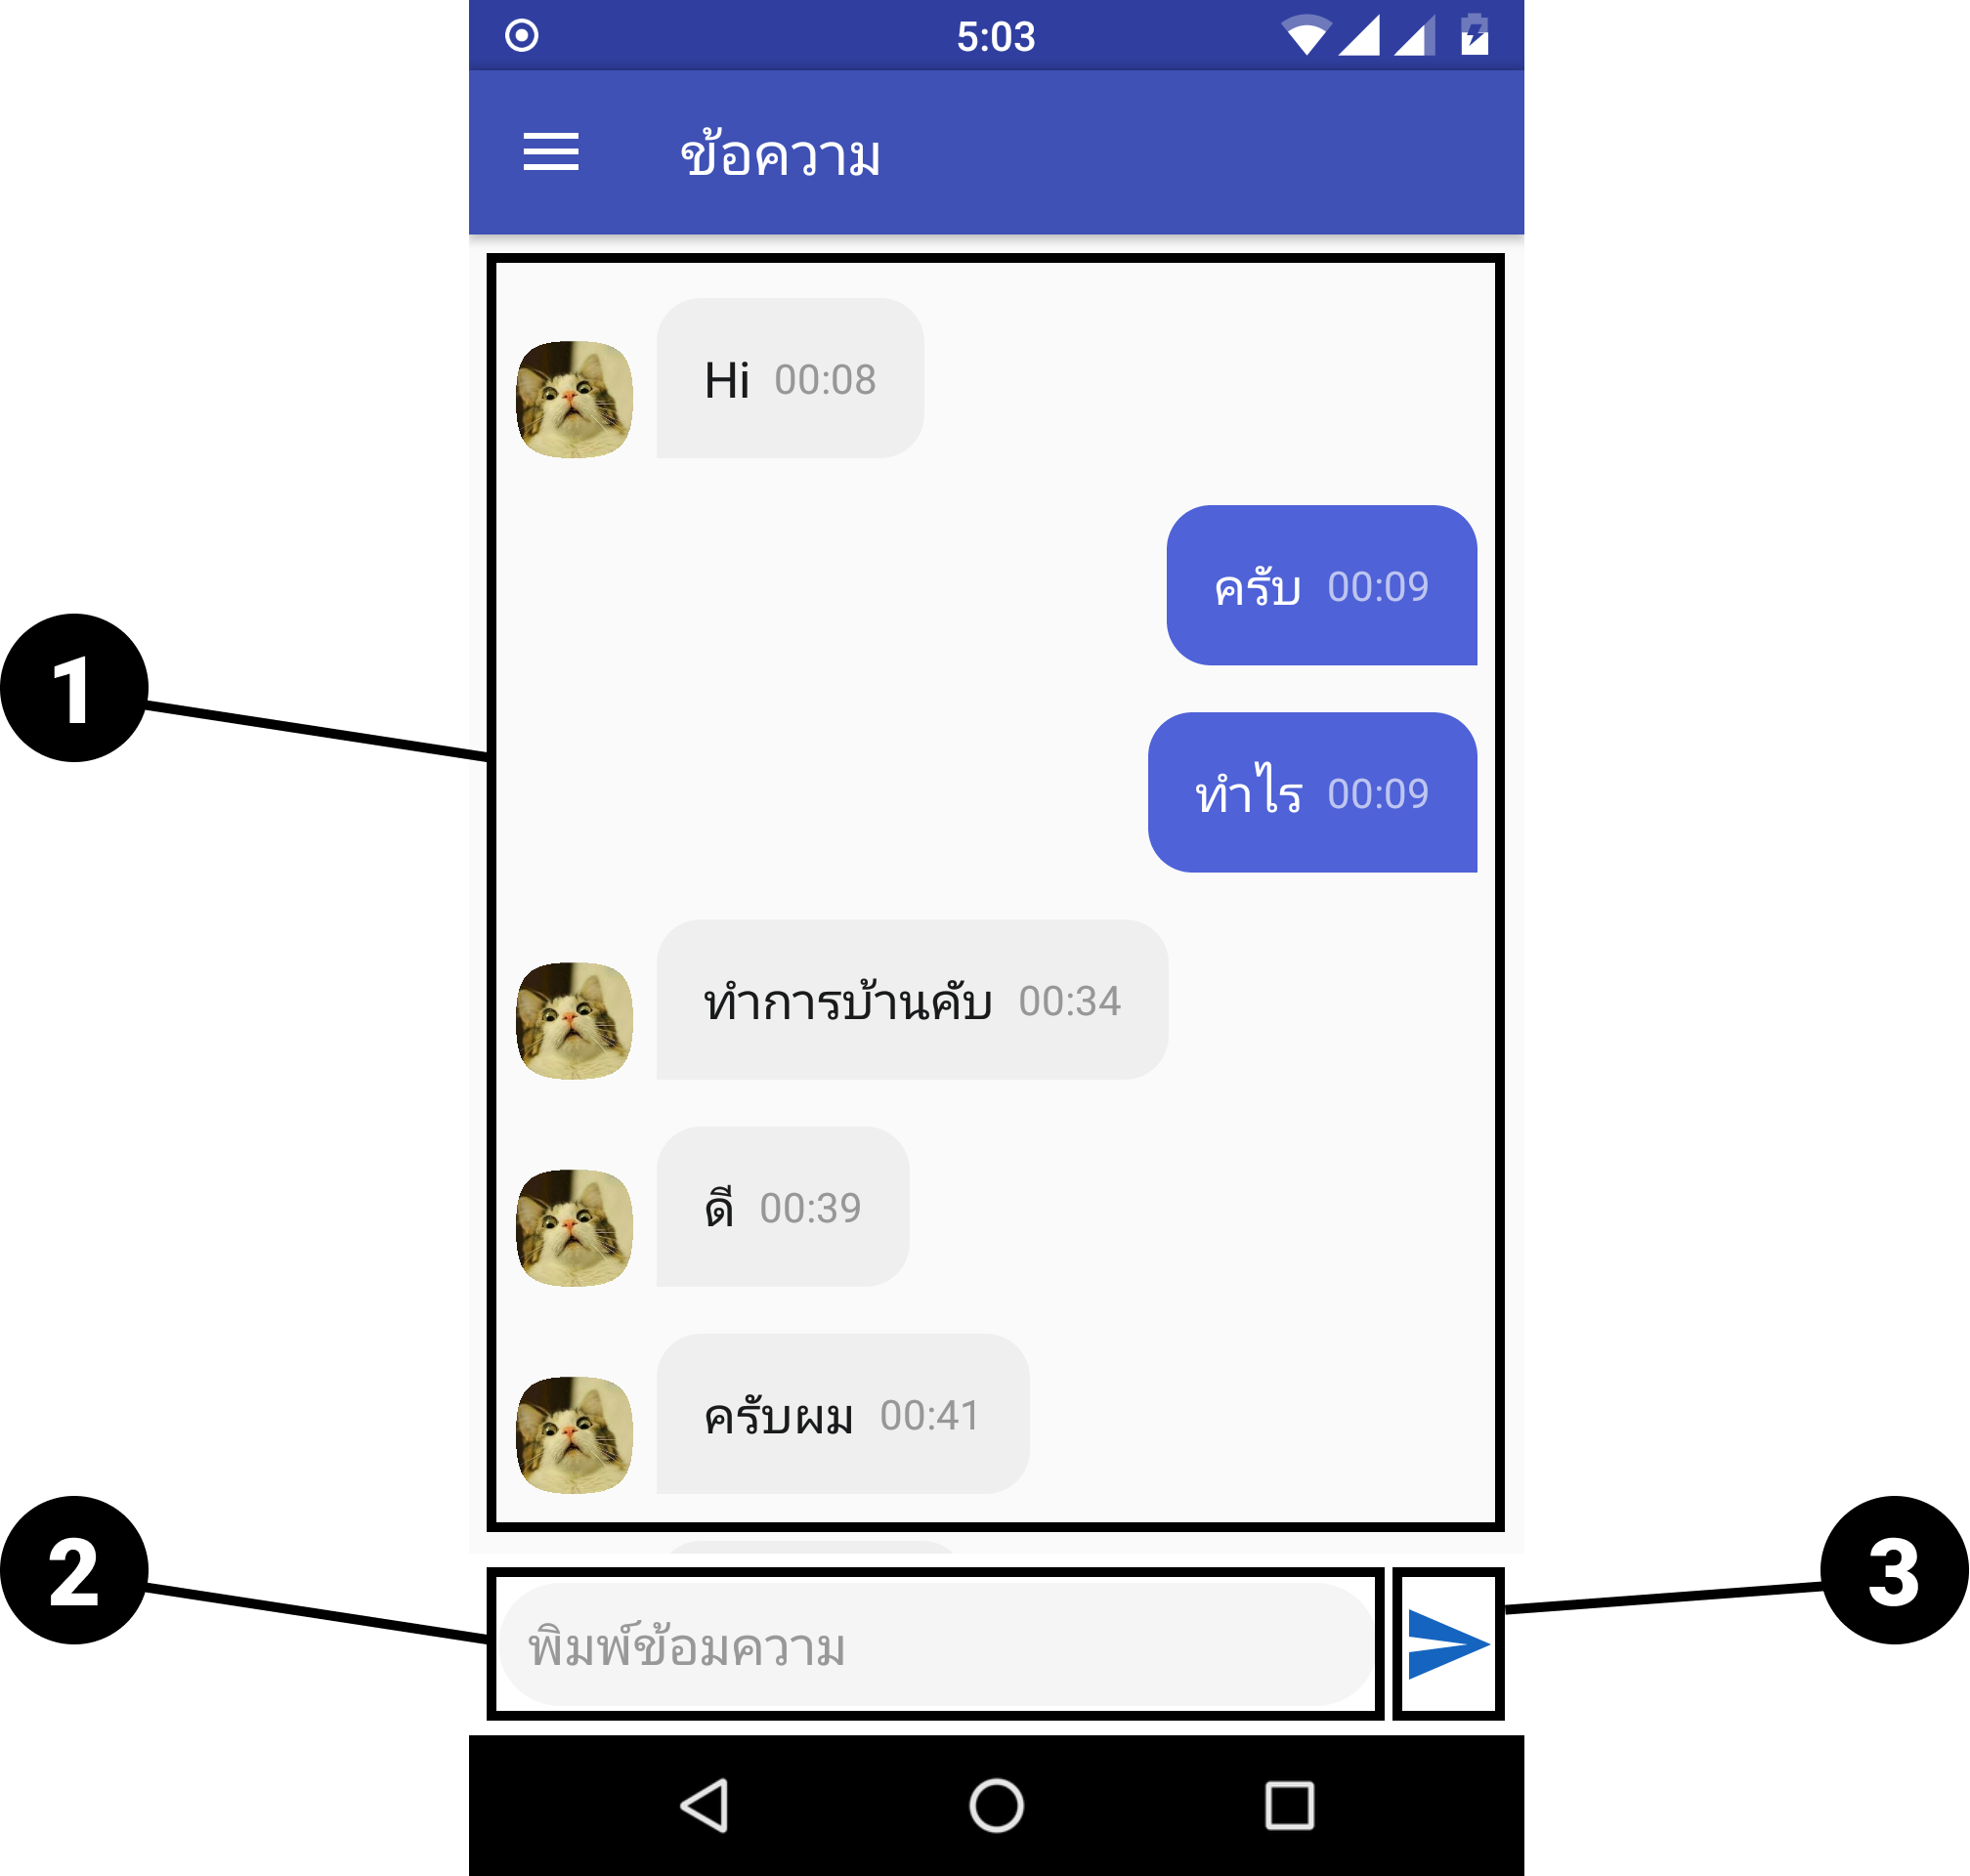
\includegraphics[width=0.5\columnwidth]{Figures/7/Manual/chat}
				\caption{หน้าจอสนทนา}
				\label{Fig:chat}
			\end{figure}
			จากรูปที่ \ref{Fig:chat} สามารถอธิบายการใช้งานได้ดังนี้
			\begin{itemize}[label={--}]
				\item หมายเลข 1 คือ รายการประวัติการสนทนา
				\item หมายเลข 2 คือ ช่องกรอกข้อความเพื่อสนทนา
				\item หมายเลข 3 คือ ปุ่มส่งข้อความ
			\end{itemize}
		
			\item เมื่อผู้ใช้เลือกเมนูส่งเอกสารระบบจะตรวจสอบข้อมูลว่าเจ้าหน้าที่ได้ทำการเปิดให้นักศึกษาส่งเอกสารได้หรือไม่ หากตรวจสอบแล้วพบว่าสามารถส่งได้ระบบจะแสดงหน้าจอส่งเอกสาร ดังแสดงในรูปที่ \ref{Fig:submit}
			\begin{figure}[H]
				\centering
				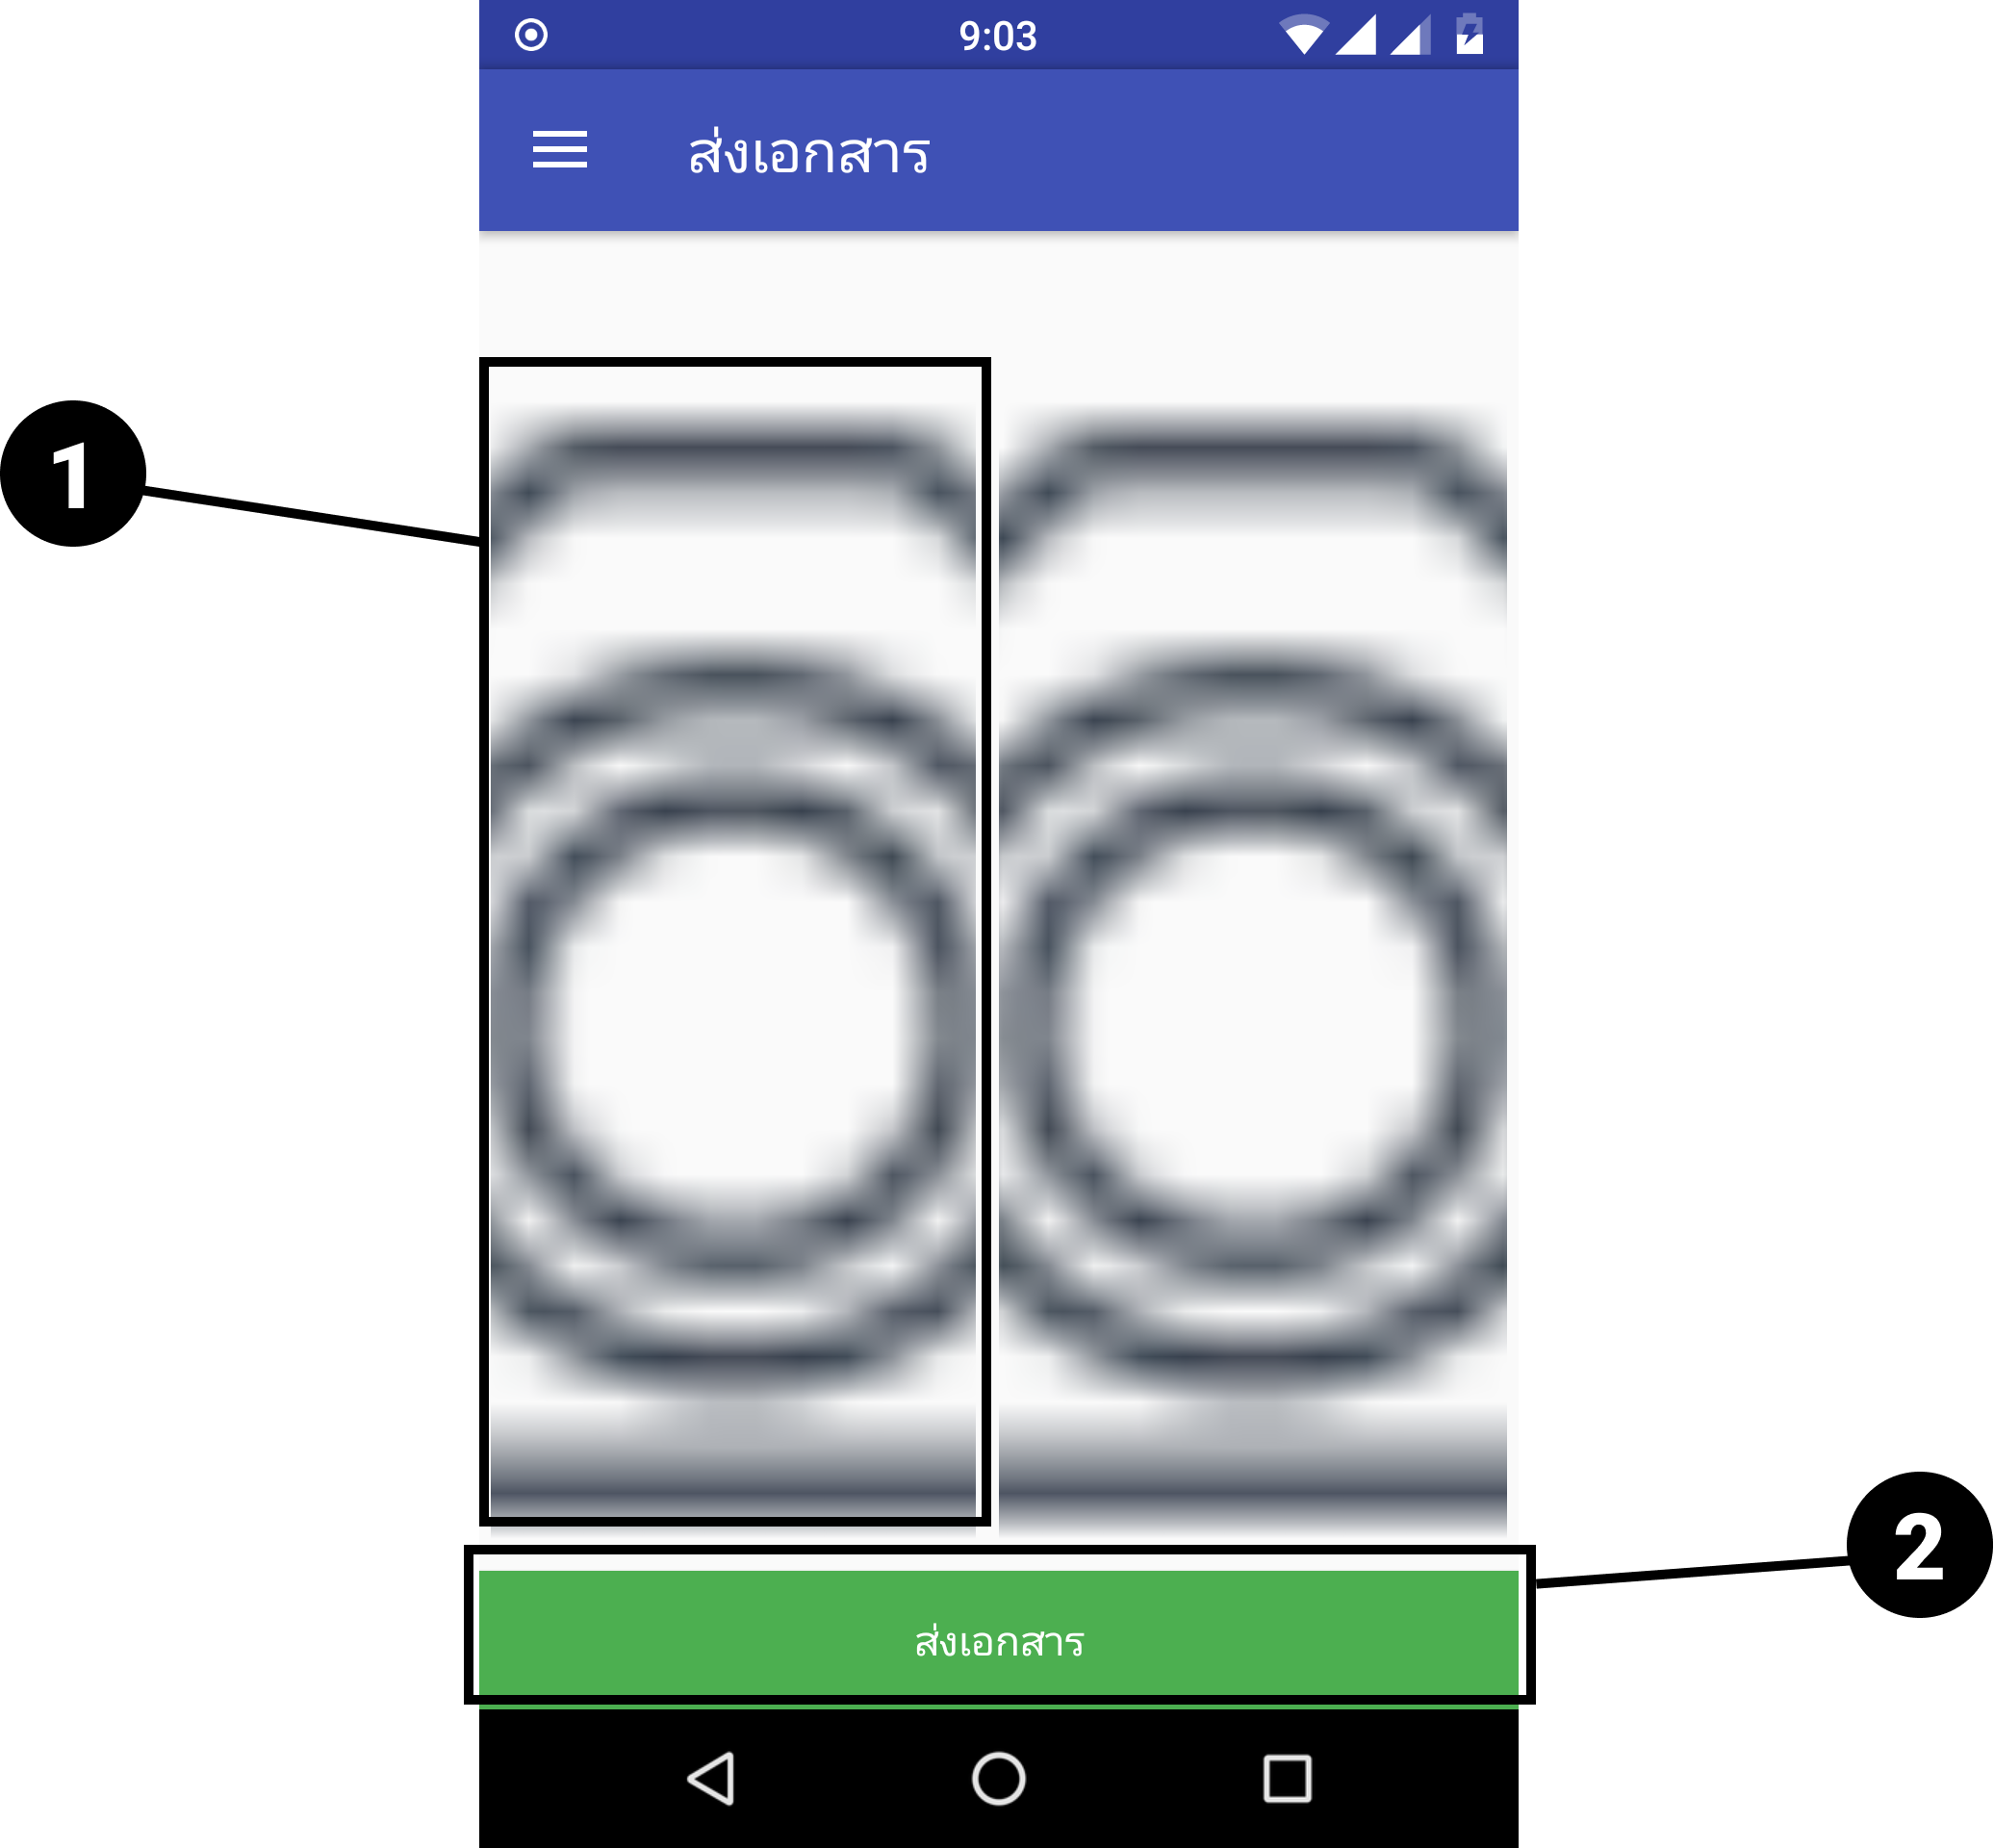
\includegraphics[width=0.5\columnwidth]{Figures/7/Manual/submit}
				\caption{หน้าจอส่งเอกสาร}
				\label{Fig:submit}
			\end{figure}
			จากรูปที่ \ref{Fig:submit} สามารถอธิบายการใช้งานได้ดังนี้
			\begin{itemize}[label={--}]
				\item หมายเลข 1 คือ เมื่อผู้ใช้เข้ามาครั้งแรกเมื่อผู้ใช้กดรูปภาพเอกสารระบบจะนำผู้ใช้ไปยังหน้าจอถ่ายภาพเอกสารและแสดงรูปภาพพรีวิว(Preview)ภาพถ่ายเอกสาร
				\item หมายเลข 2 คือ ปุ่มกดส่งเอกสาร
			\end{itemize}
		
			\item เมื่อผู้ใช้กดที่ปุ่มถ่ายภาพเอกสารระบบจะแสดงหน้าจอถ่ายภาพเอกสาร ดังแสดงในรูปที่ \ref{Fig:submit1}
			\begin{figure}[H]
				\centering
				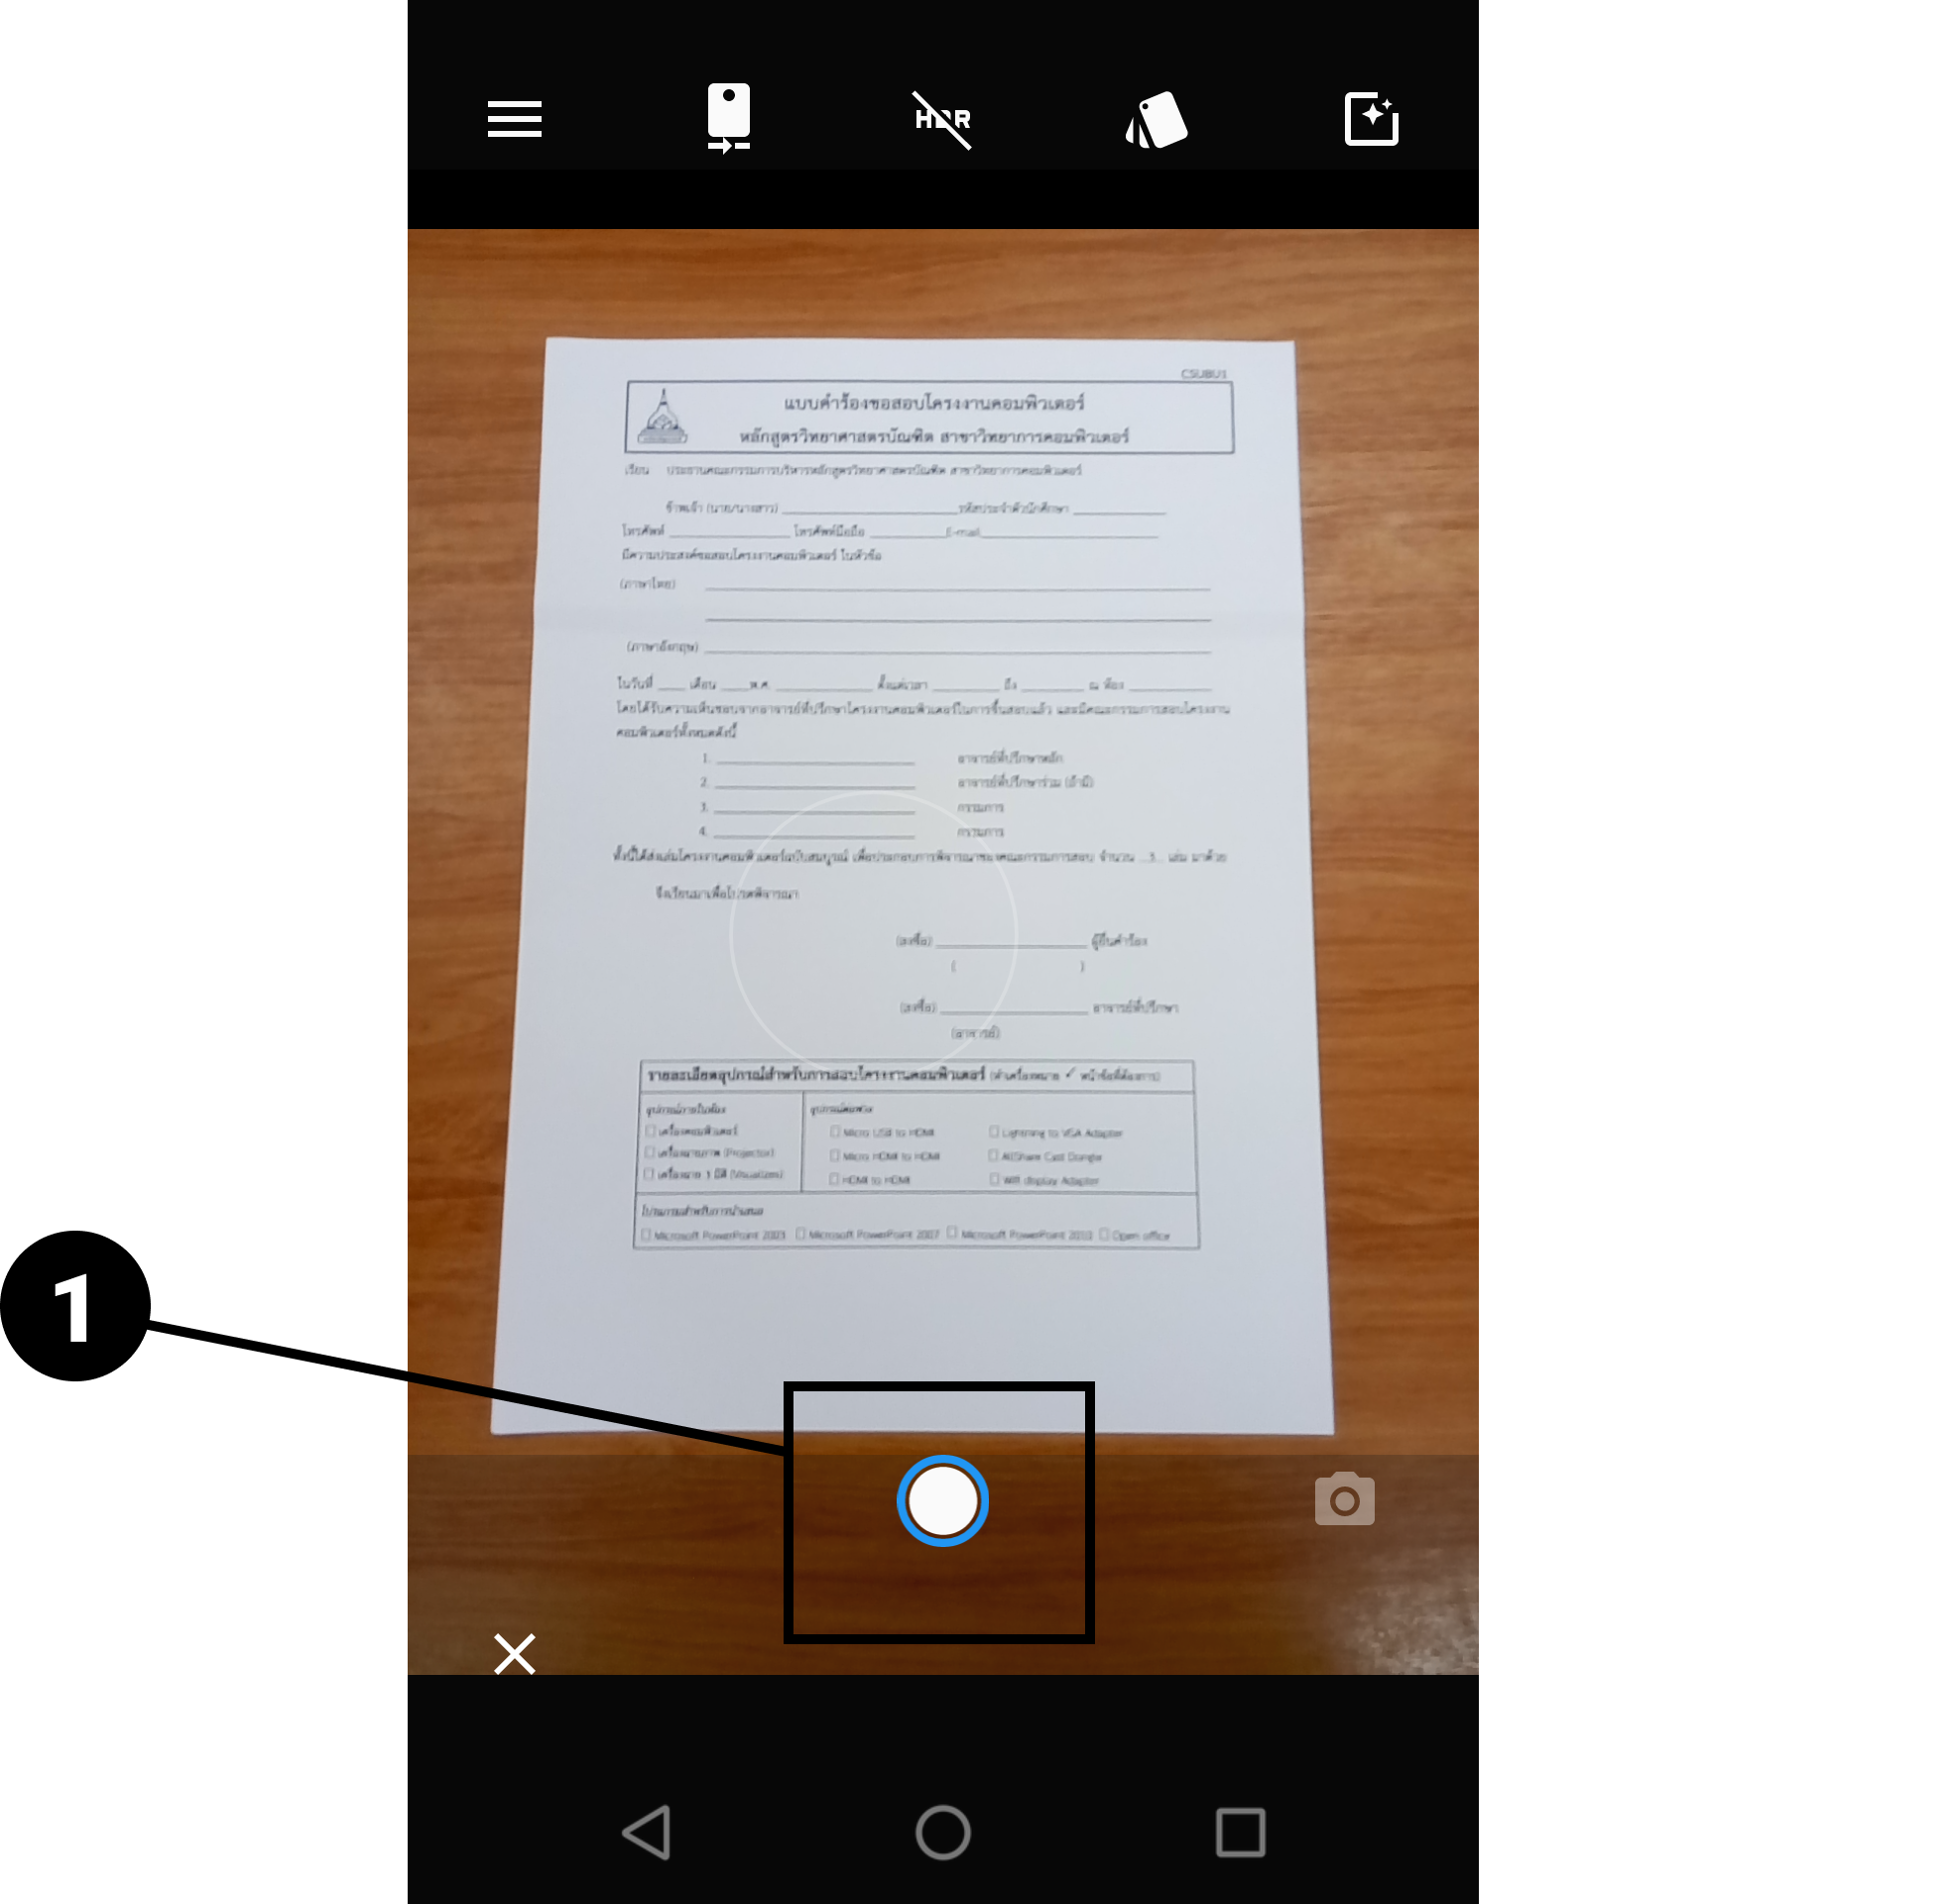
\includegraphics[width=0.5\columnwidth]{Figures/7/Manual/submit1}
				\caption{หน้าจอถ่ายภาพเอกสาร}
				\label{Fig:submit1}
			\end{figure}
			จากรูปที่ \ref{Fig:submit1} สามารถอธิบายการใช้งานได้ดังนี้
			\begin{itemize}[label={--}]
				\item หมายเลข 1 คือ ปุ่มกดถ่ายภาพสำเนาเอกสาร
			\end{itemize}
		
			\item หน้าจอแสดงภาพพรีวิวภาพถ่ายสำเนาเอกสาร ดังแสดงในรูปที่ \ref{Fig:submit2}
			\begin{figure}[H]
				\centering
				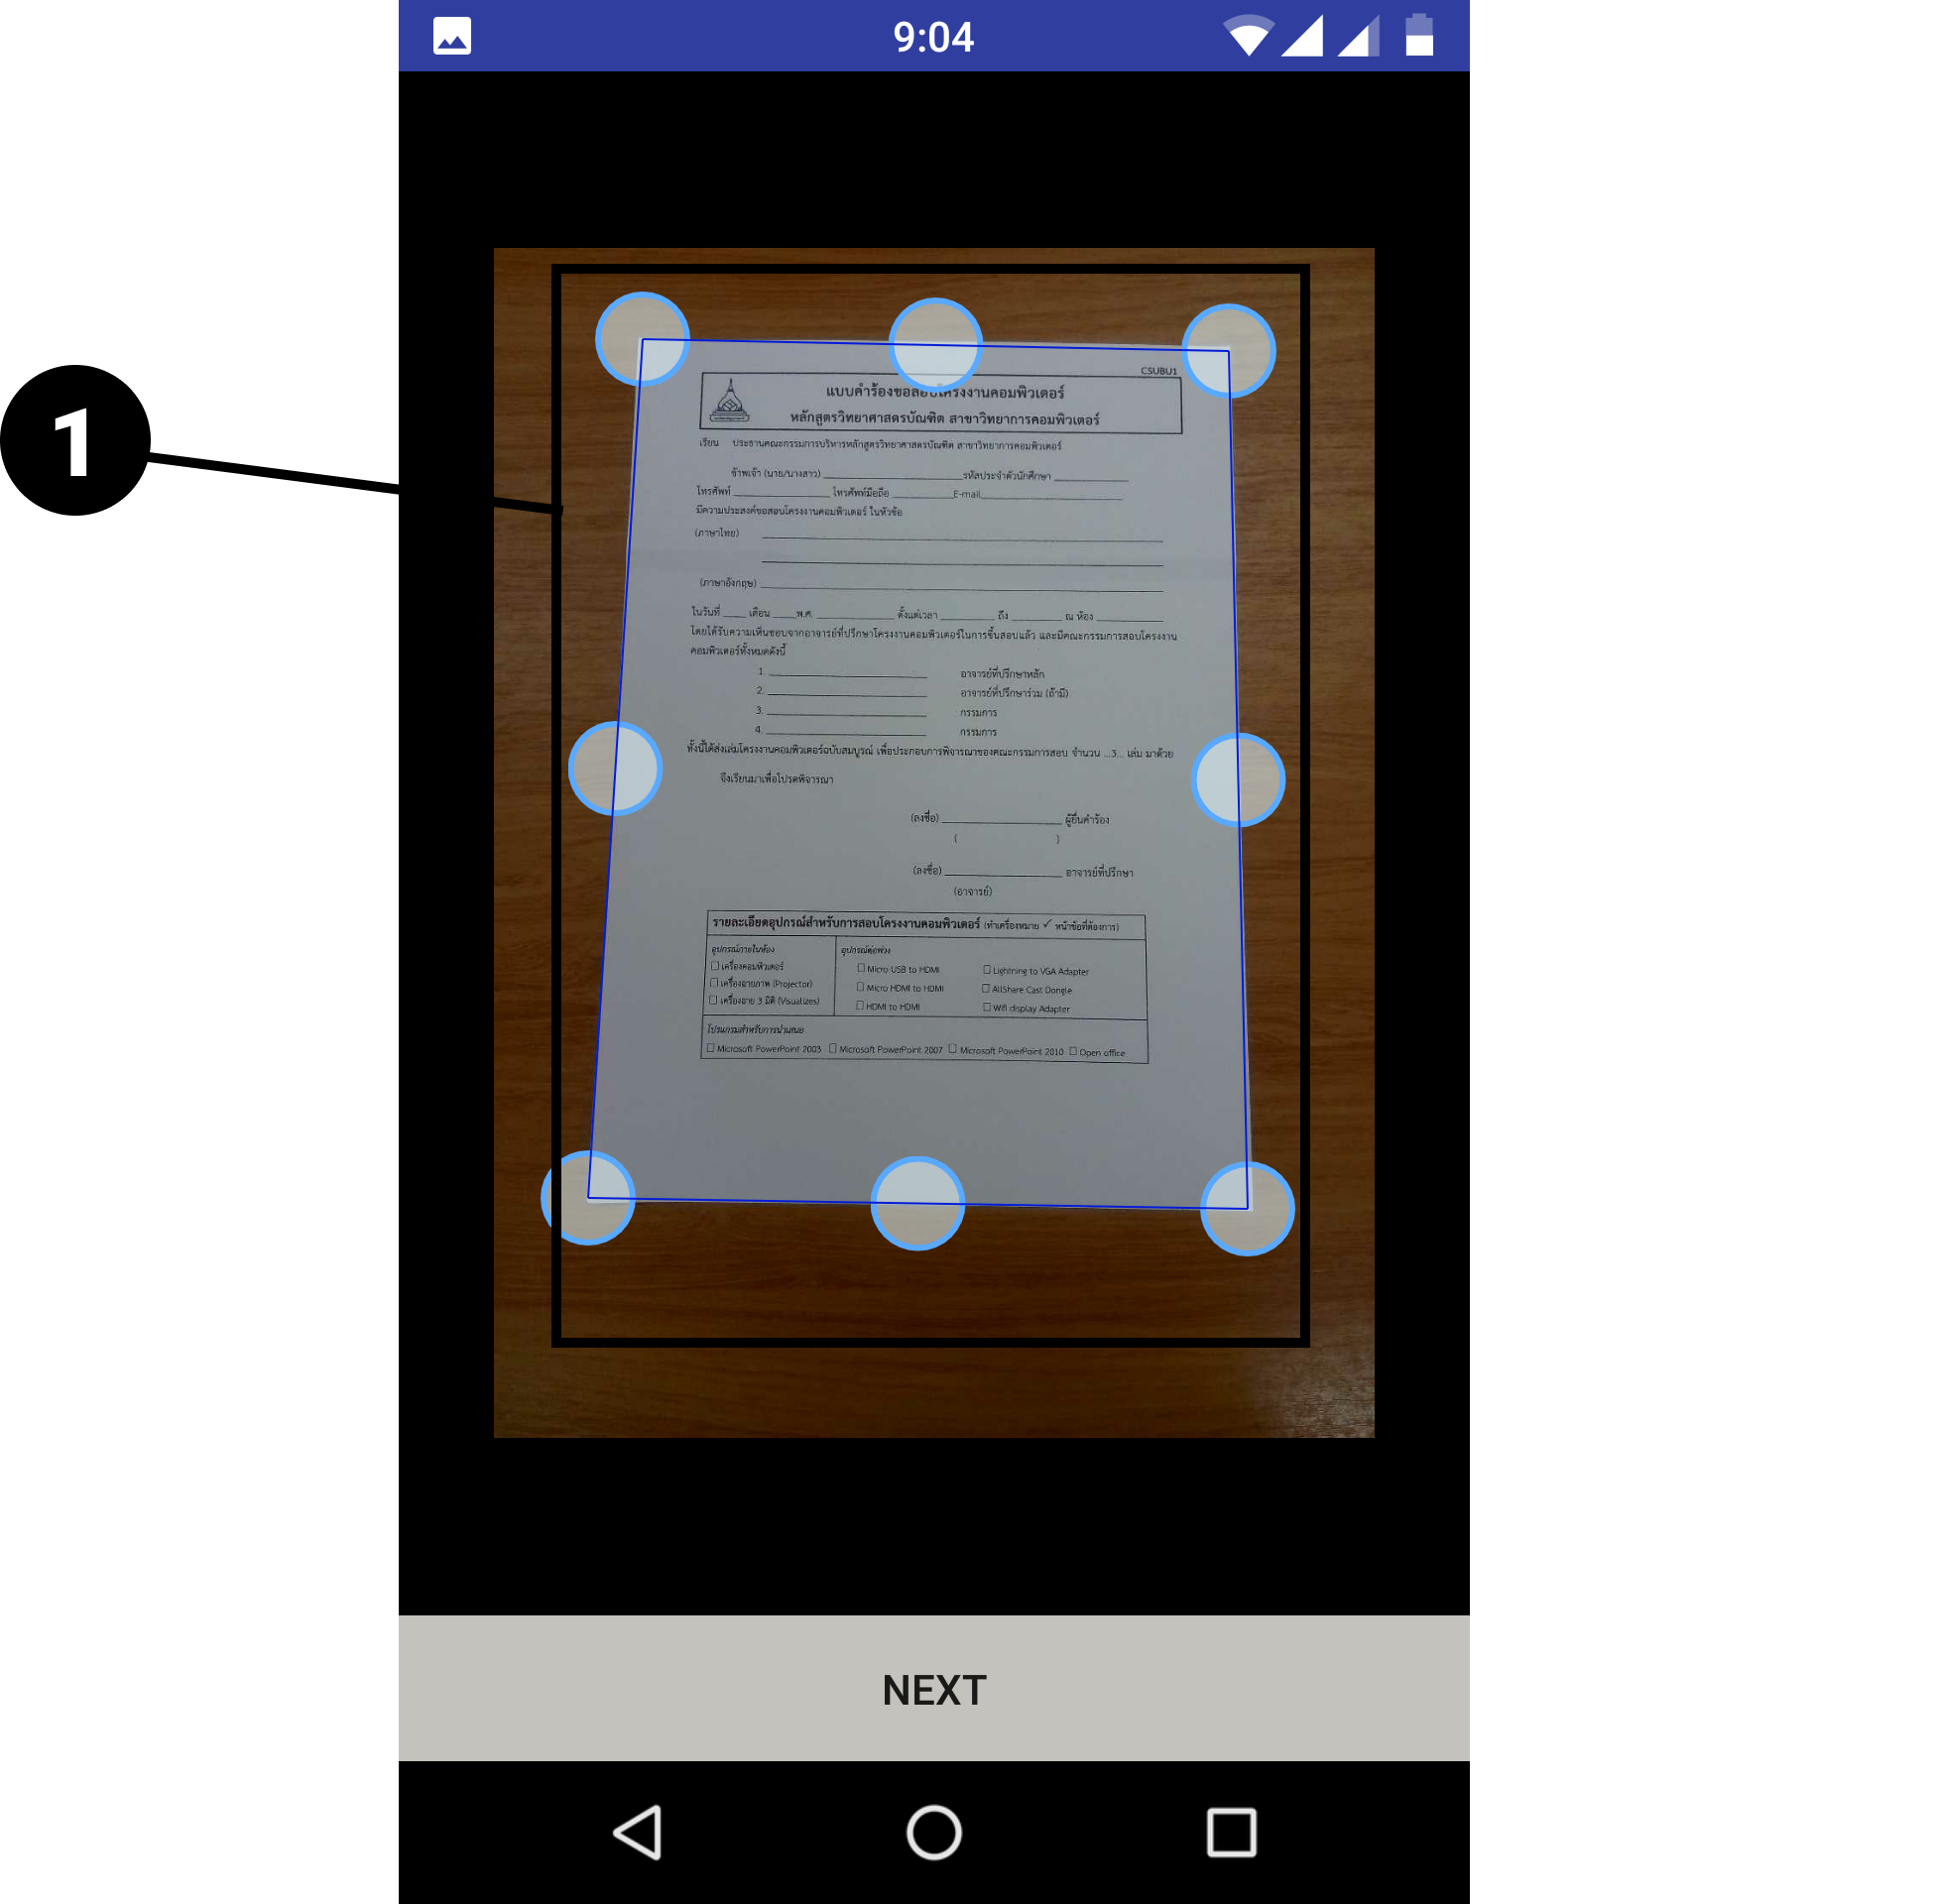
\includegraphics[width=0.5\columnwidth]{Figures/7/Manual/submit2}
				\caption{หน้าจอแสดงภาพพรีวิวภาพถ่ายสำเนาเอกสาร}
				\label{Fig:submit2}
			\end{figure}
			จากรูปที่ \ref{Fig:submit2} สามารถอธิบายการใช้งานได้ดังนี้
			\begin{itemize}[label={--}]
				\item หมายเลข 1 คือ ปุ่มปรับมุมภาพทั้ง 8 มุมเพื่อปรับขนาดภาพถ่ายเอกสาร
			\end{itemize}
			
			\item หน้าจอแสดงปรับแต่งภาพถ่ายสำเนาเอกสาร ดังแสดงในรูปที่ \ref{Fig:submit3}
			\begin{figure}[H]
				\centering
				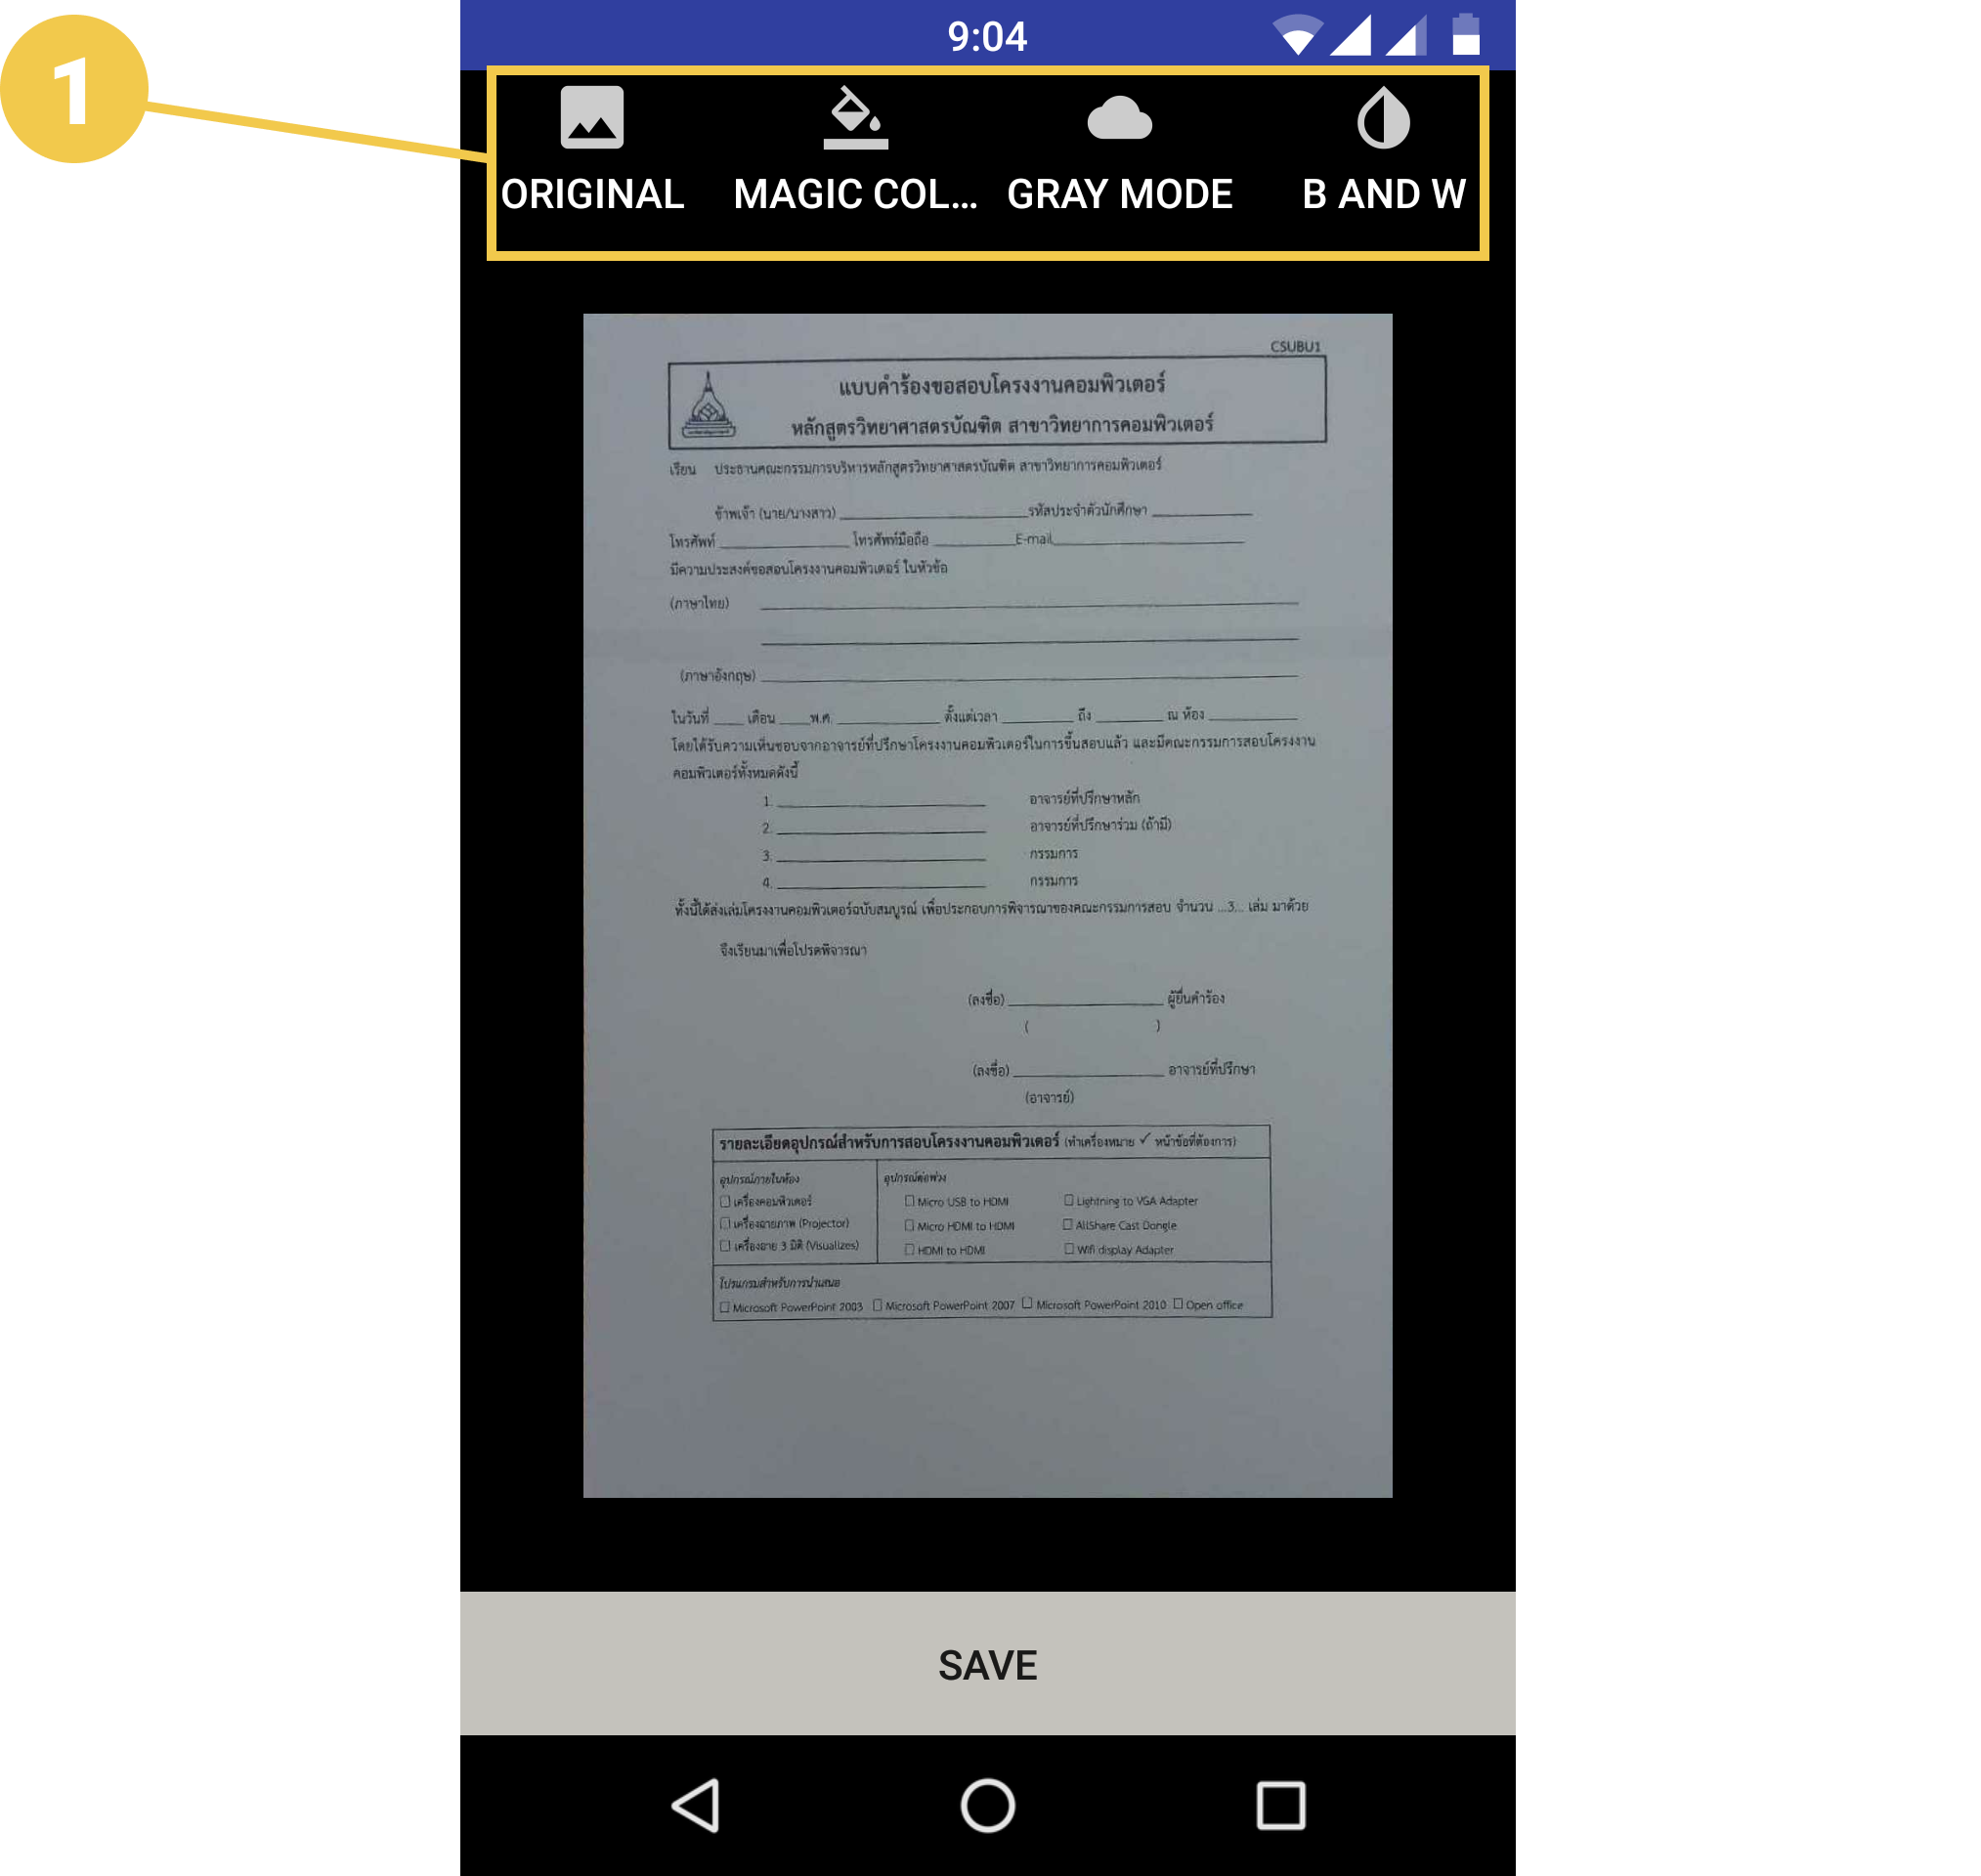
\includegraphics[width=0.5\columnwidth]{Figures/7/Manual/submit3}
				\caption{หน้าจอแสดงปรับแต่งภาพถ่ายสำเนาเอกสาร}
				\label{Fig:submit3}
			\end{figure}
			จากรูปที่ \ref{Fig:submit3} สามารถอธิบายการใช้งานได้ดังนี้
			\begin{itemize}[label={--}]
				\item หมายเลข 1 คือ เมื่อผู้ใช้ต้องการปรับความคมชัดของภาพสามารถทำได้จาก 4 ปุ่ม คือ ปุ่มภาพต้นฉบับ ปุ่มปรับสีอัตโนมัติ ปุ่มปรับปรับสีเป็นสีเทา ปุ่มปรับสีเป็นสีขาวดำ
			\end{itemize} 
		
			\item หน้าจอแสดงภาพพรีวิวภาพถ่ายสำเนาเอกสารทั้งสองฉบับ ดังแสดงในรูปที่ \ref{Fig:submit4}
			\begin{figure}[H]
				\centering
				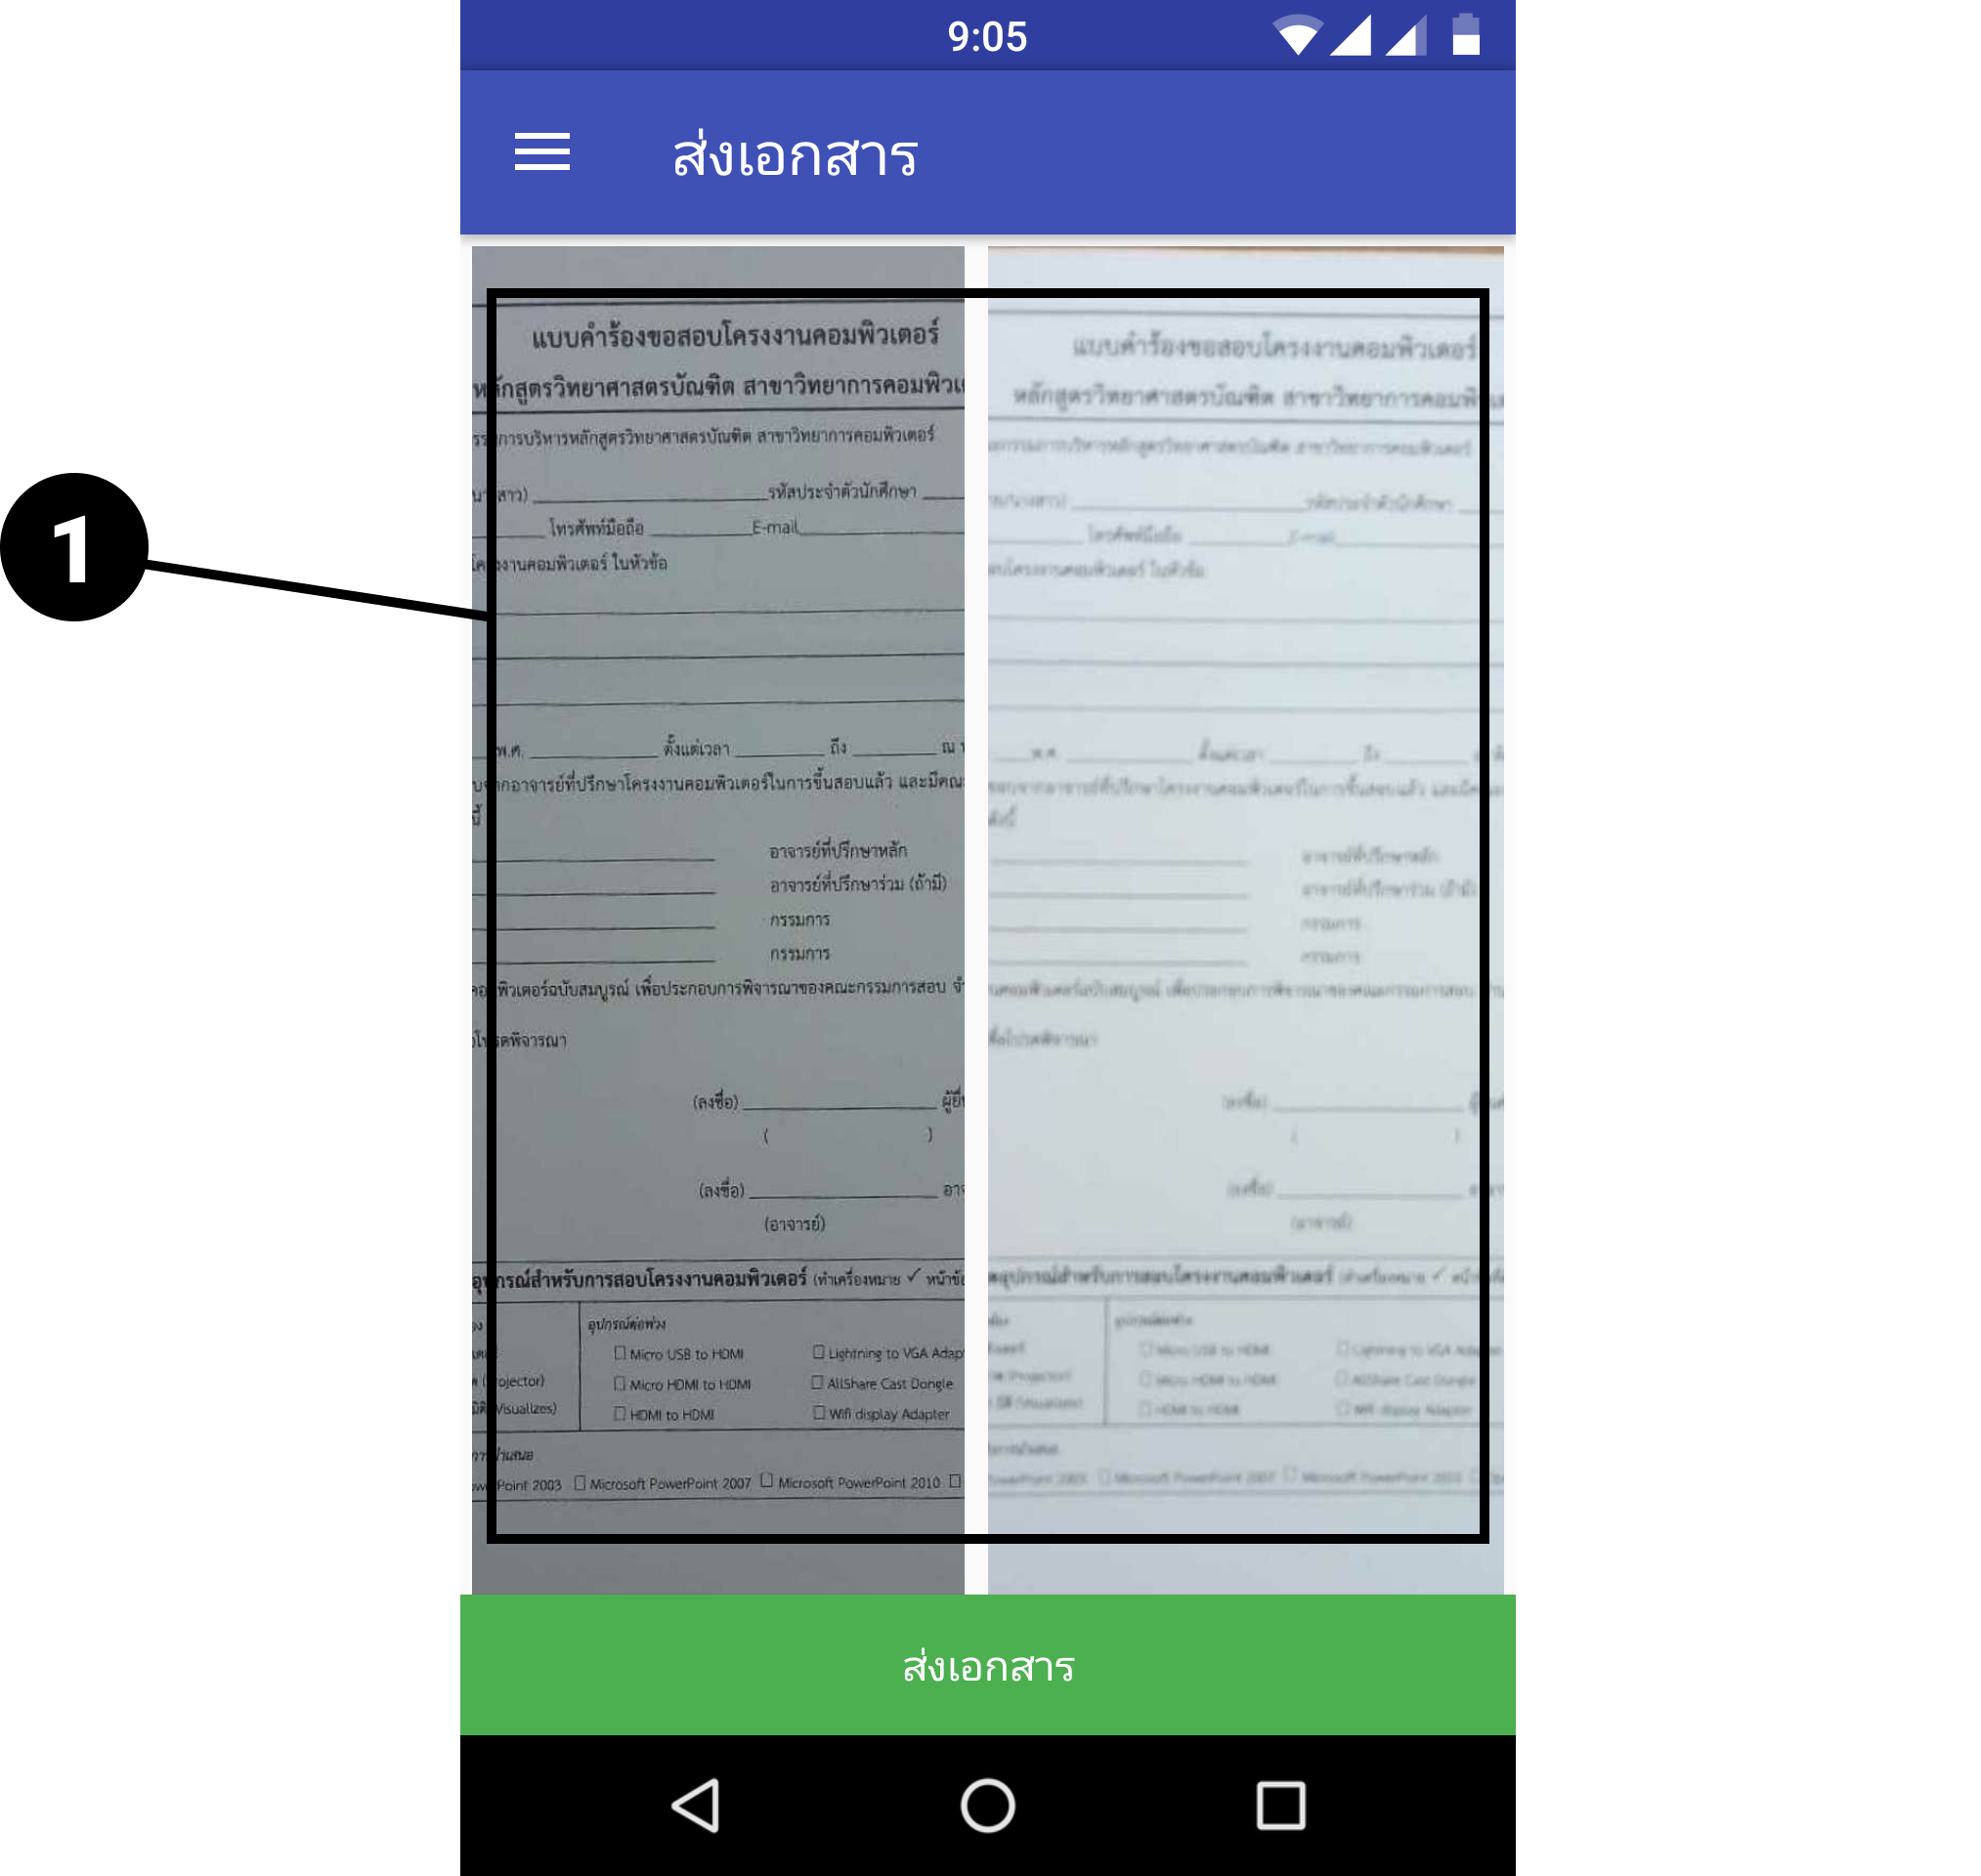
\includegraphics[width=0.5\columnwidth]{Figures/7/Manual/submit4}
				\caption{หน้าจอแสดงภาพพรีวิวภาพถ่ายสำเนาเอกสาร}
				\label{Fig:submit4}
			\end{figure}
			จากรูปที่ \ref{Fig:submit4} สามารถอธิบายการใช้งานได้ดังนี้
			\begin{itemize}[label={--}]
				\item หมายเลข 1 คือ แสดงภาพพรีวิวภาพถ่ายสำเนาเอกสารทั้งสองฉบับ 
			\end{itemize} 
			
			\item เมื่อผู้ใช้กดปุ่มส่งเอกสาร ระบบจะแสดงหน้าต่างแสดงสถานะการอัพโหลดเอกสาร ดังแสดงในรูปที่ \ref{Fig:submit5}
			\begin{figure}[H]
				\centering
				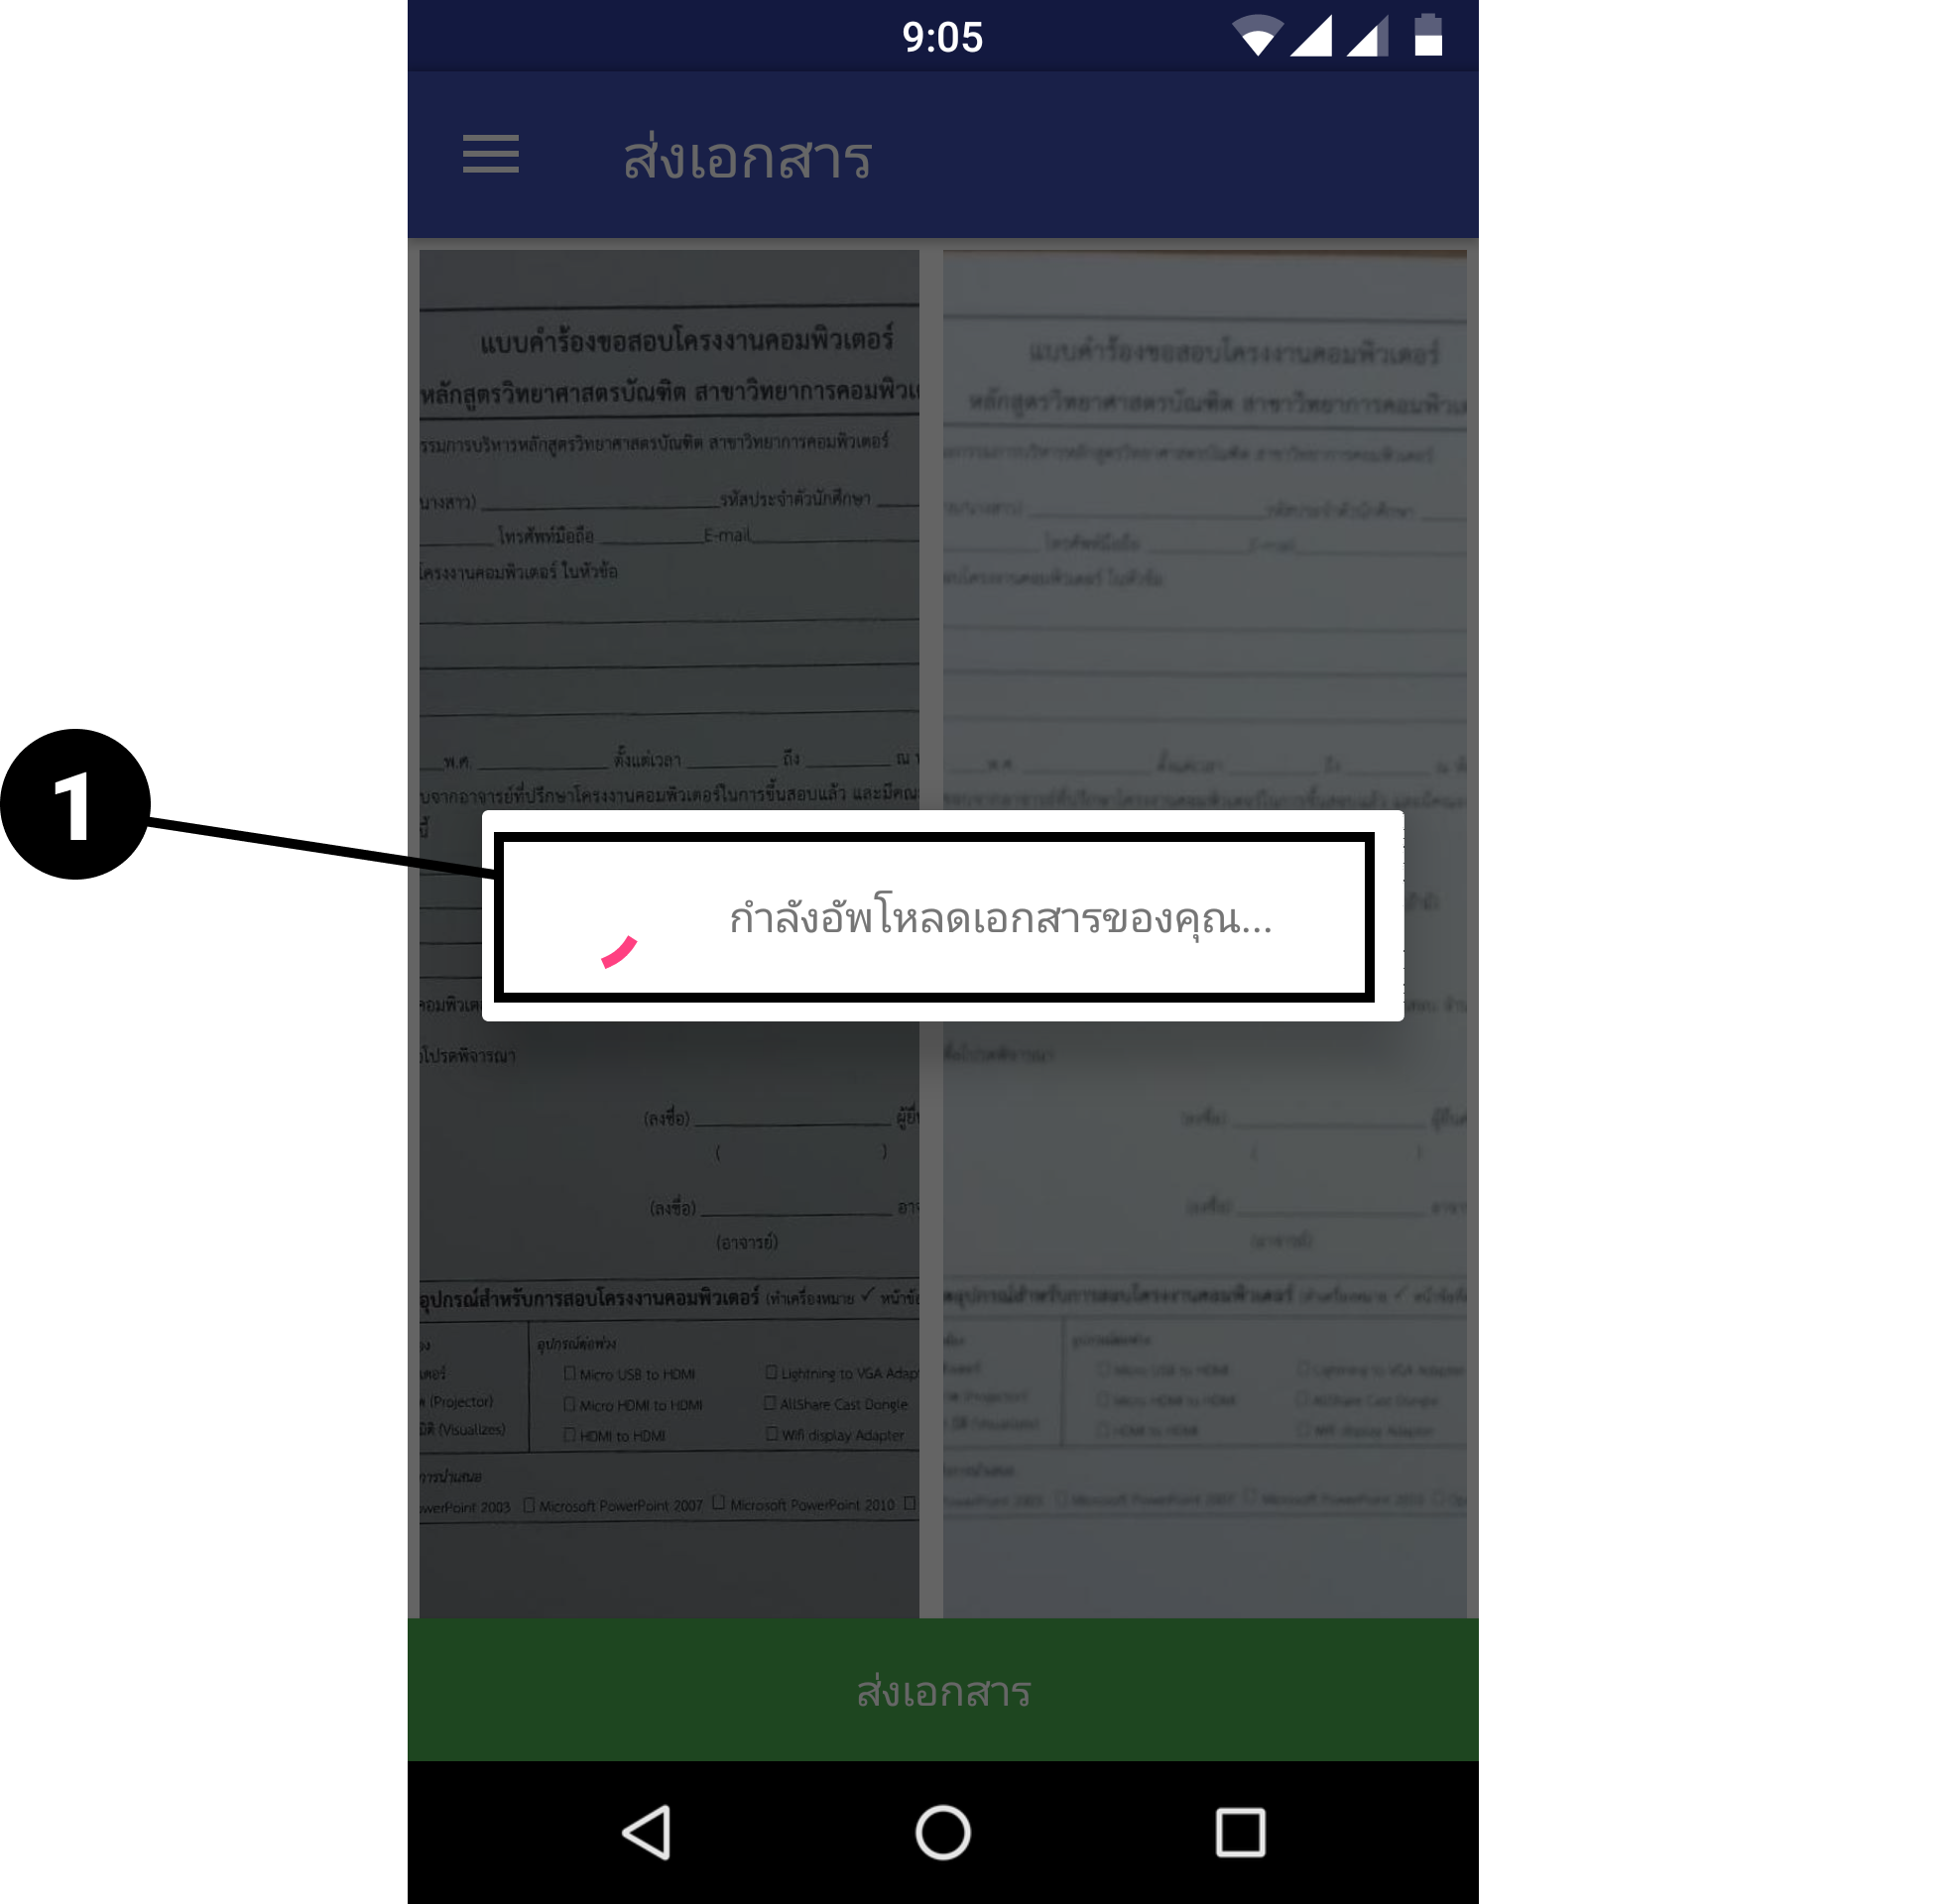
\includegraphics[width=0.5\columnwidth]{Figures/7/Manual/submit5}
				\caption{หน้าต่างแสดงสถานะการอัพโหลดเอกสาร}
				\label{Fig:submit5}
			\end{figure}
			จากรูปที่ \ref{Fig:submit5} สามารถอธิบายการใช้งานได้ดังนี้
			\begin{itemize}[label={--}]
				\item หมายเลข 1 คือ หน้าต่างสถานะการอัพโหลดเอกสาร 
			\end{itemize} 
		
			\item เมื่อผู้ใช้กดเมนูจองคิว ระบบจะตรวจสอบถสานะการส่งเอกสารว่าถูกเจ้าหน้าที่ตรวจสอบแล้วหรือไม่ ถ้าเจ้าหน้าที่อนุมัติแล้วระบบจะแสดงหน้าจอจองวันที่ส่งเอกสาร ดังแสดงในรูปที่ \ref{Fig:checkin}
			\begin{figure}[H]
				\centering
				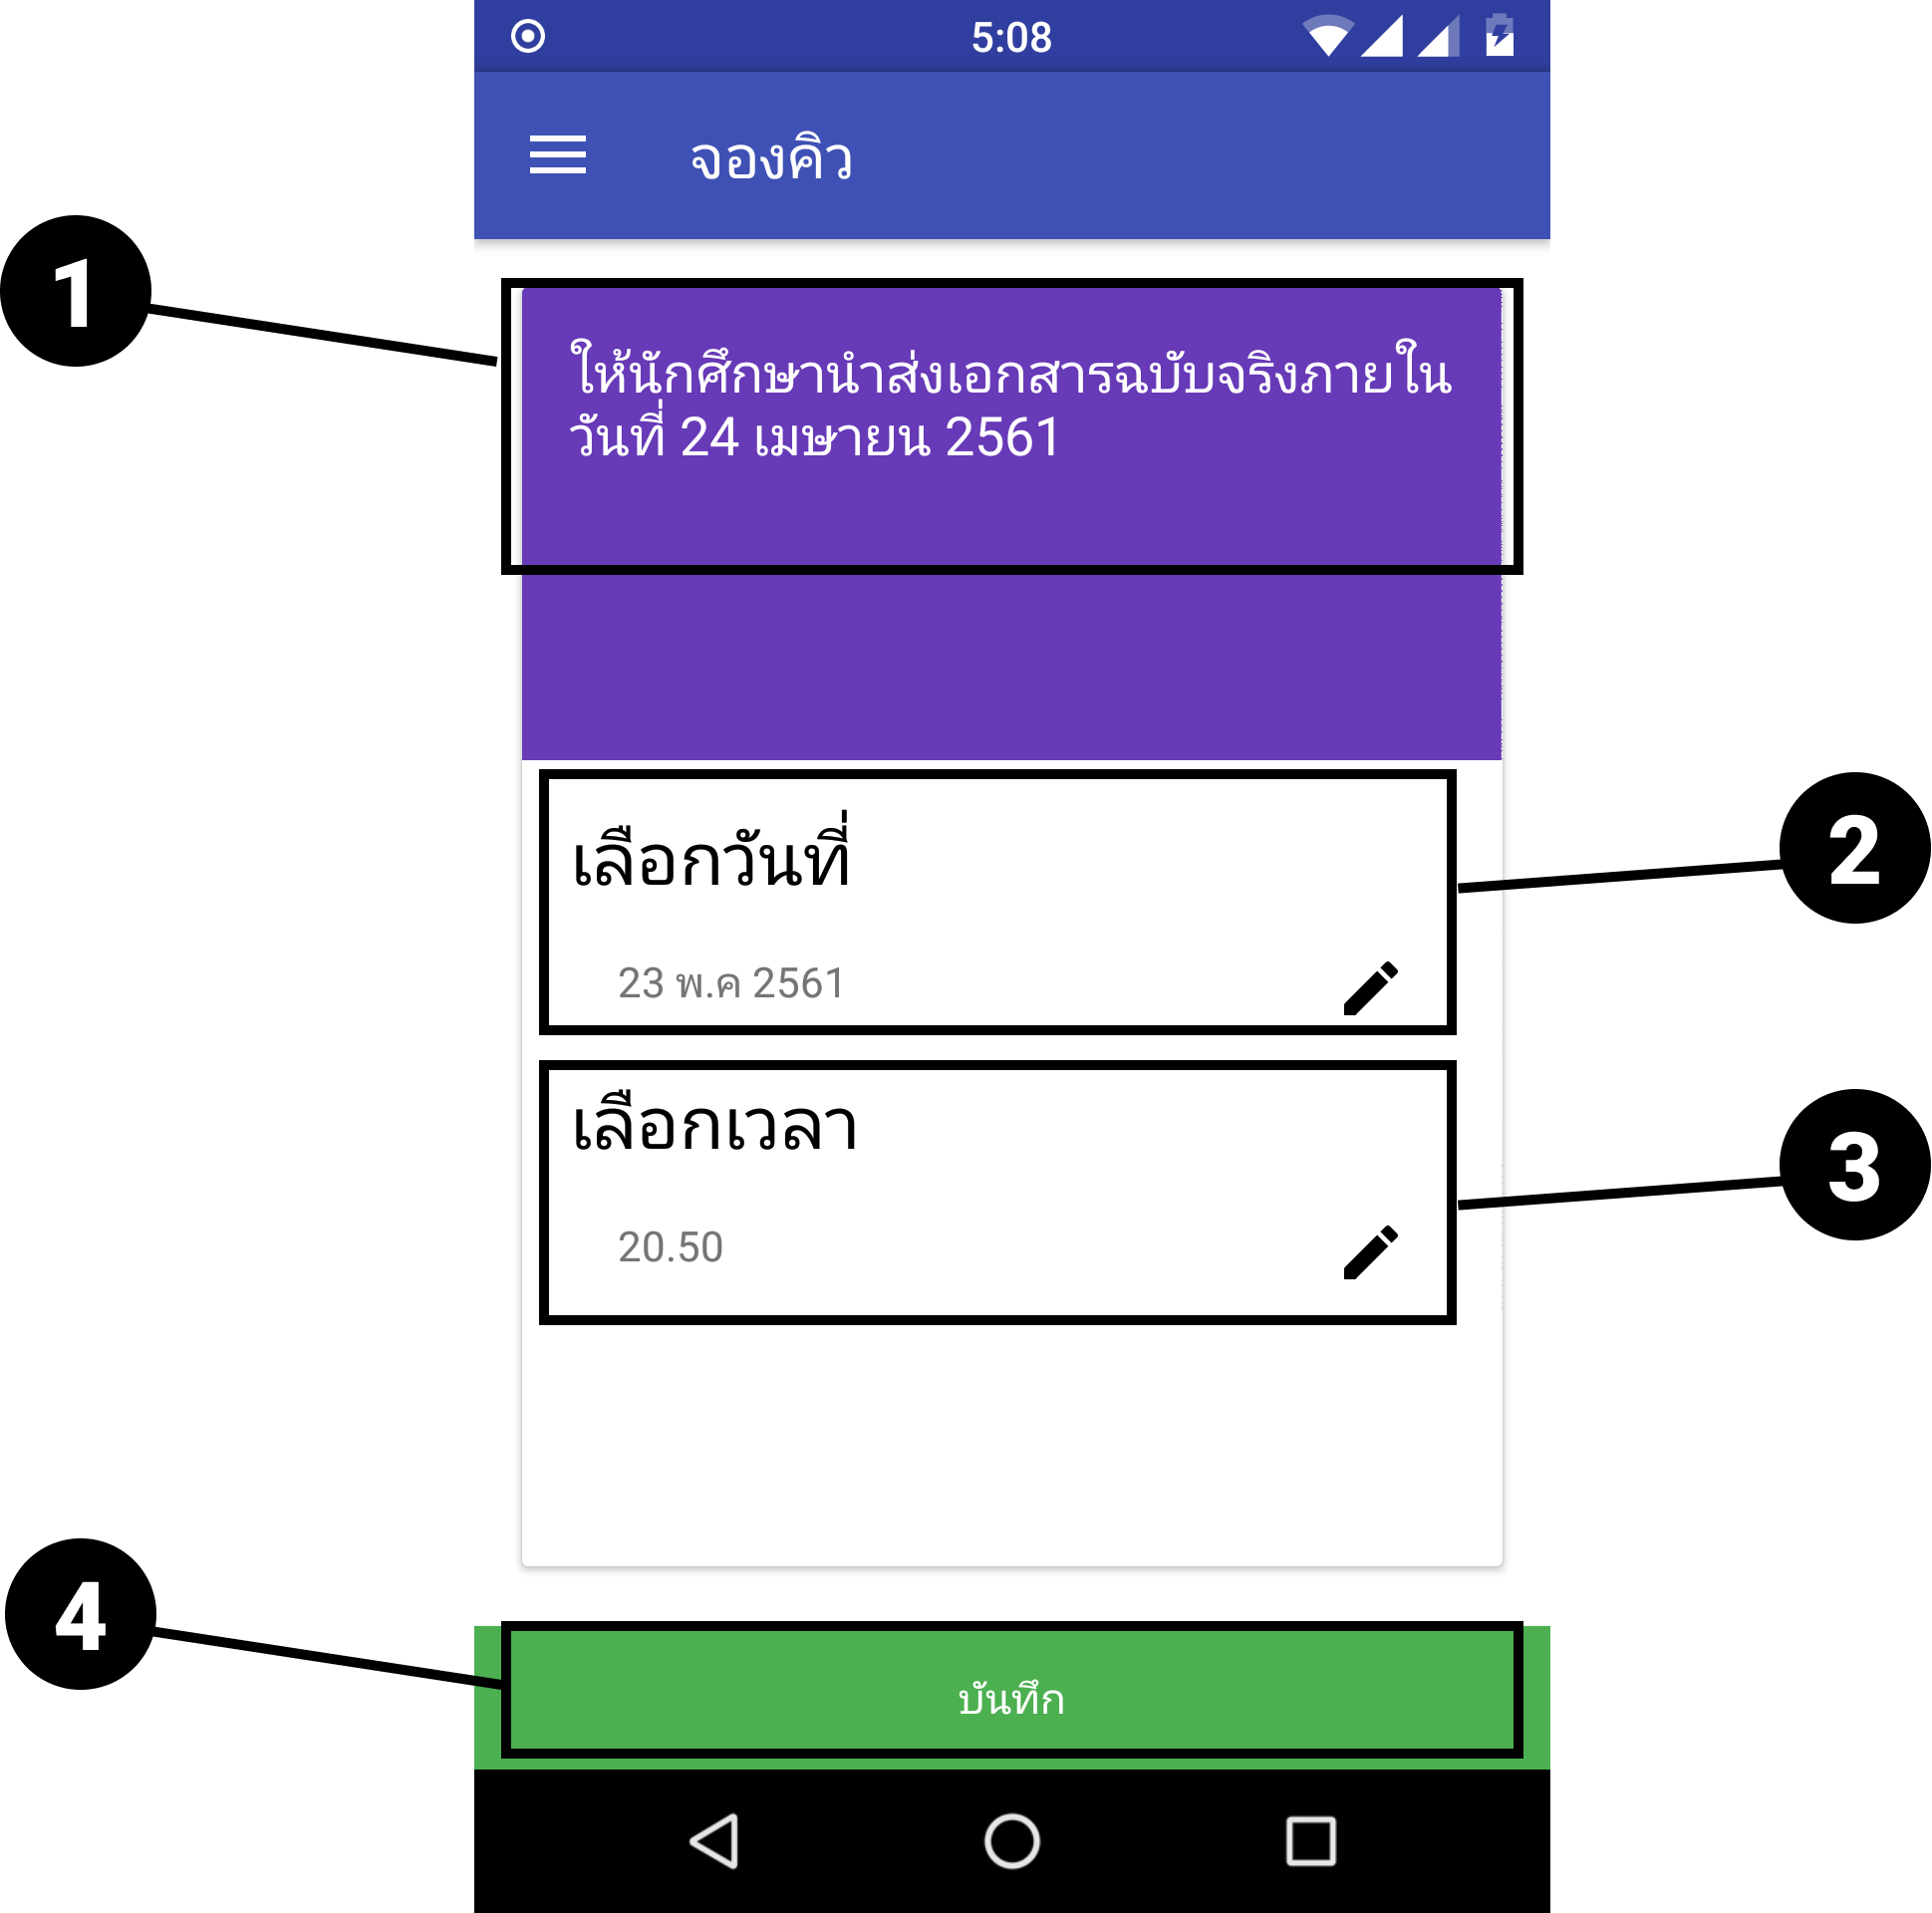
\includegraphics[width=0.5\columnwidth]{Figures/7/Manual/checkin}
				\caption{หน้าจอจองคิว}
				\label{Fig:checkin}
			\end{figure}
			จากรูปที่ \ref{Fig:checkin} สามารถอธิบายการใช้งานได้ดังนี้
			\begin{itemize}[label={--}]
				\item หมายเลข 1 คือ รายละเอียด 
				\item หมายเลข 2 คือ ส่วนของการเลือกวันที่ที่ต้องการส่งเอกสาร
				\item หมายเลข 3 คือ ส่วนของการเลือกเวลาที่ต้องการส่งเอกสาร
				\item หมายเลข 4 คือ ปุ่มกดส่งเอกสาร
			\end{itemize} 
		
			\item เมื่อผู้ใช้กดปุ่มเลือกวันที่ที่ต้องการส่งเอกสารระบบจะแสดงหน้าต่างเลือกวันที่โดยจะแสดงเฉพาะวันที่ที่เจ้าหน้าที่เลือกไว้เท่านั้น ดังแสดงในรูปที่ \ref{Fig:date}
			\begin{figure}[H]
				\centering
				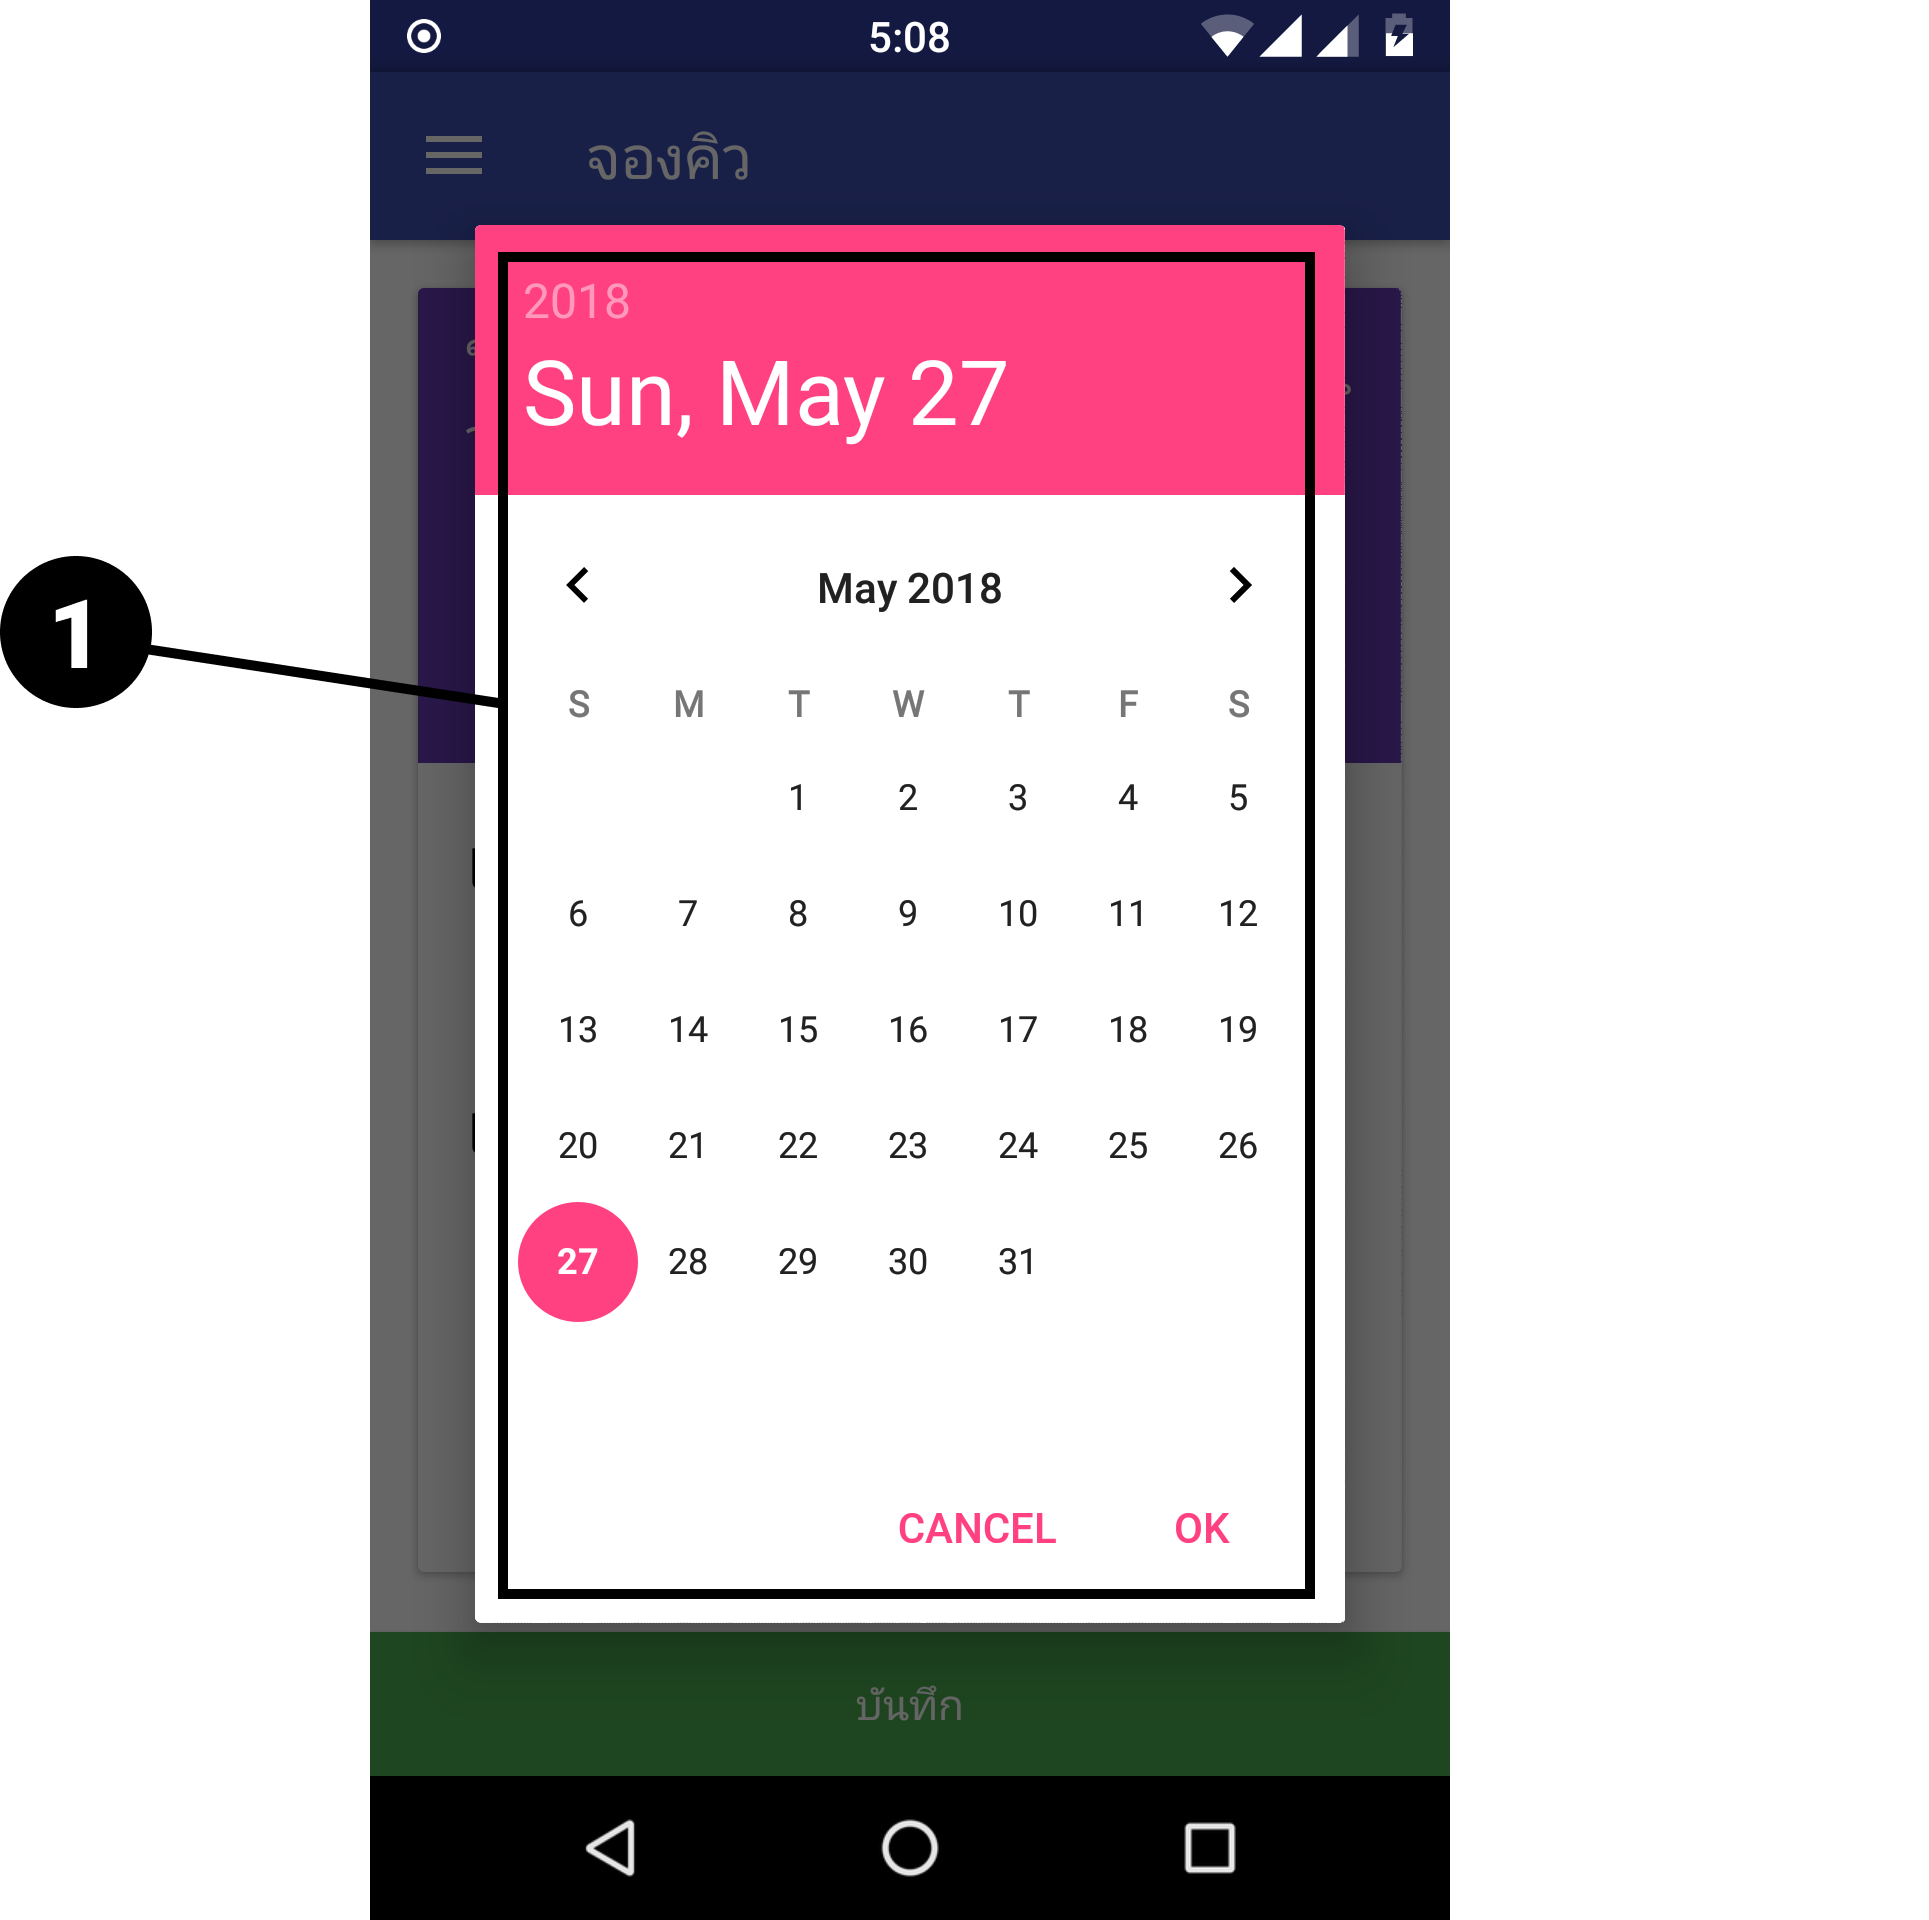
\includegraphics[width=0.5\columnwidth]{Figures/7/Manual/date}
				\caption{หน้าต่างปฏิทินเลือกวันที่ต้องการส่งเอกสาร}
				\label{Fig:date}
			\end{figure}
			จากรูปที่ \ref{Fig:date} สามารถอธิบายการใช้งานได้ดังนี้
			\begin{itemize}[label={--}]
				\item หมายเลข 1 คือ หน้าต่างปฏิทินเลือกวันที่ต้องการส่งเอกสาร 
			\end{itemize}
			
			\item เมื่อผู้ใช้กดปุ่มเลือกเวลาที่ต้องการส่งเอกสารระบบจะแสดงหน้าต่างเลือกเวลาโดยจะแสดงเฉพาะเวลาที่เจ้าหน้าที่เลือกไว้เท่านั้น ดังแสดงในรูปที่ \ref{Fig:time}
			\begin{figure}[H]
				\centering
				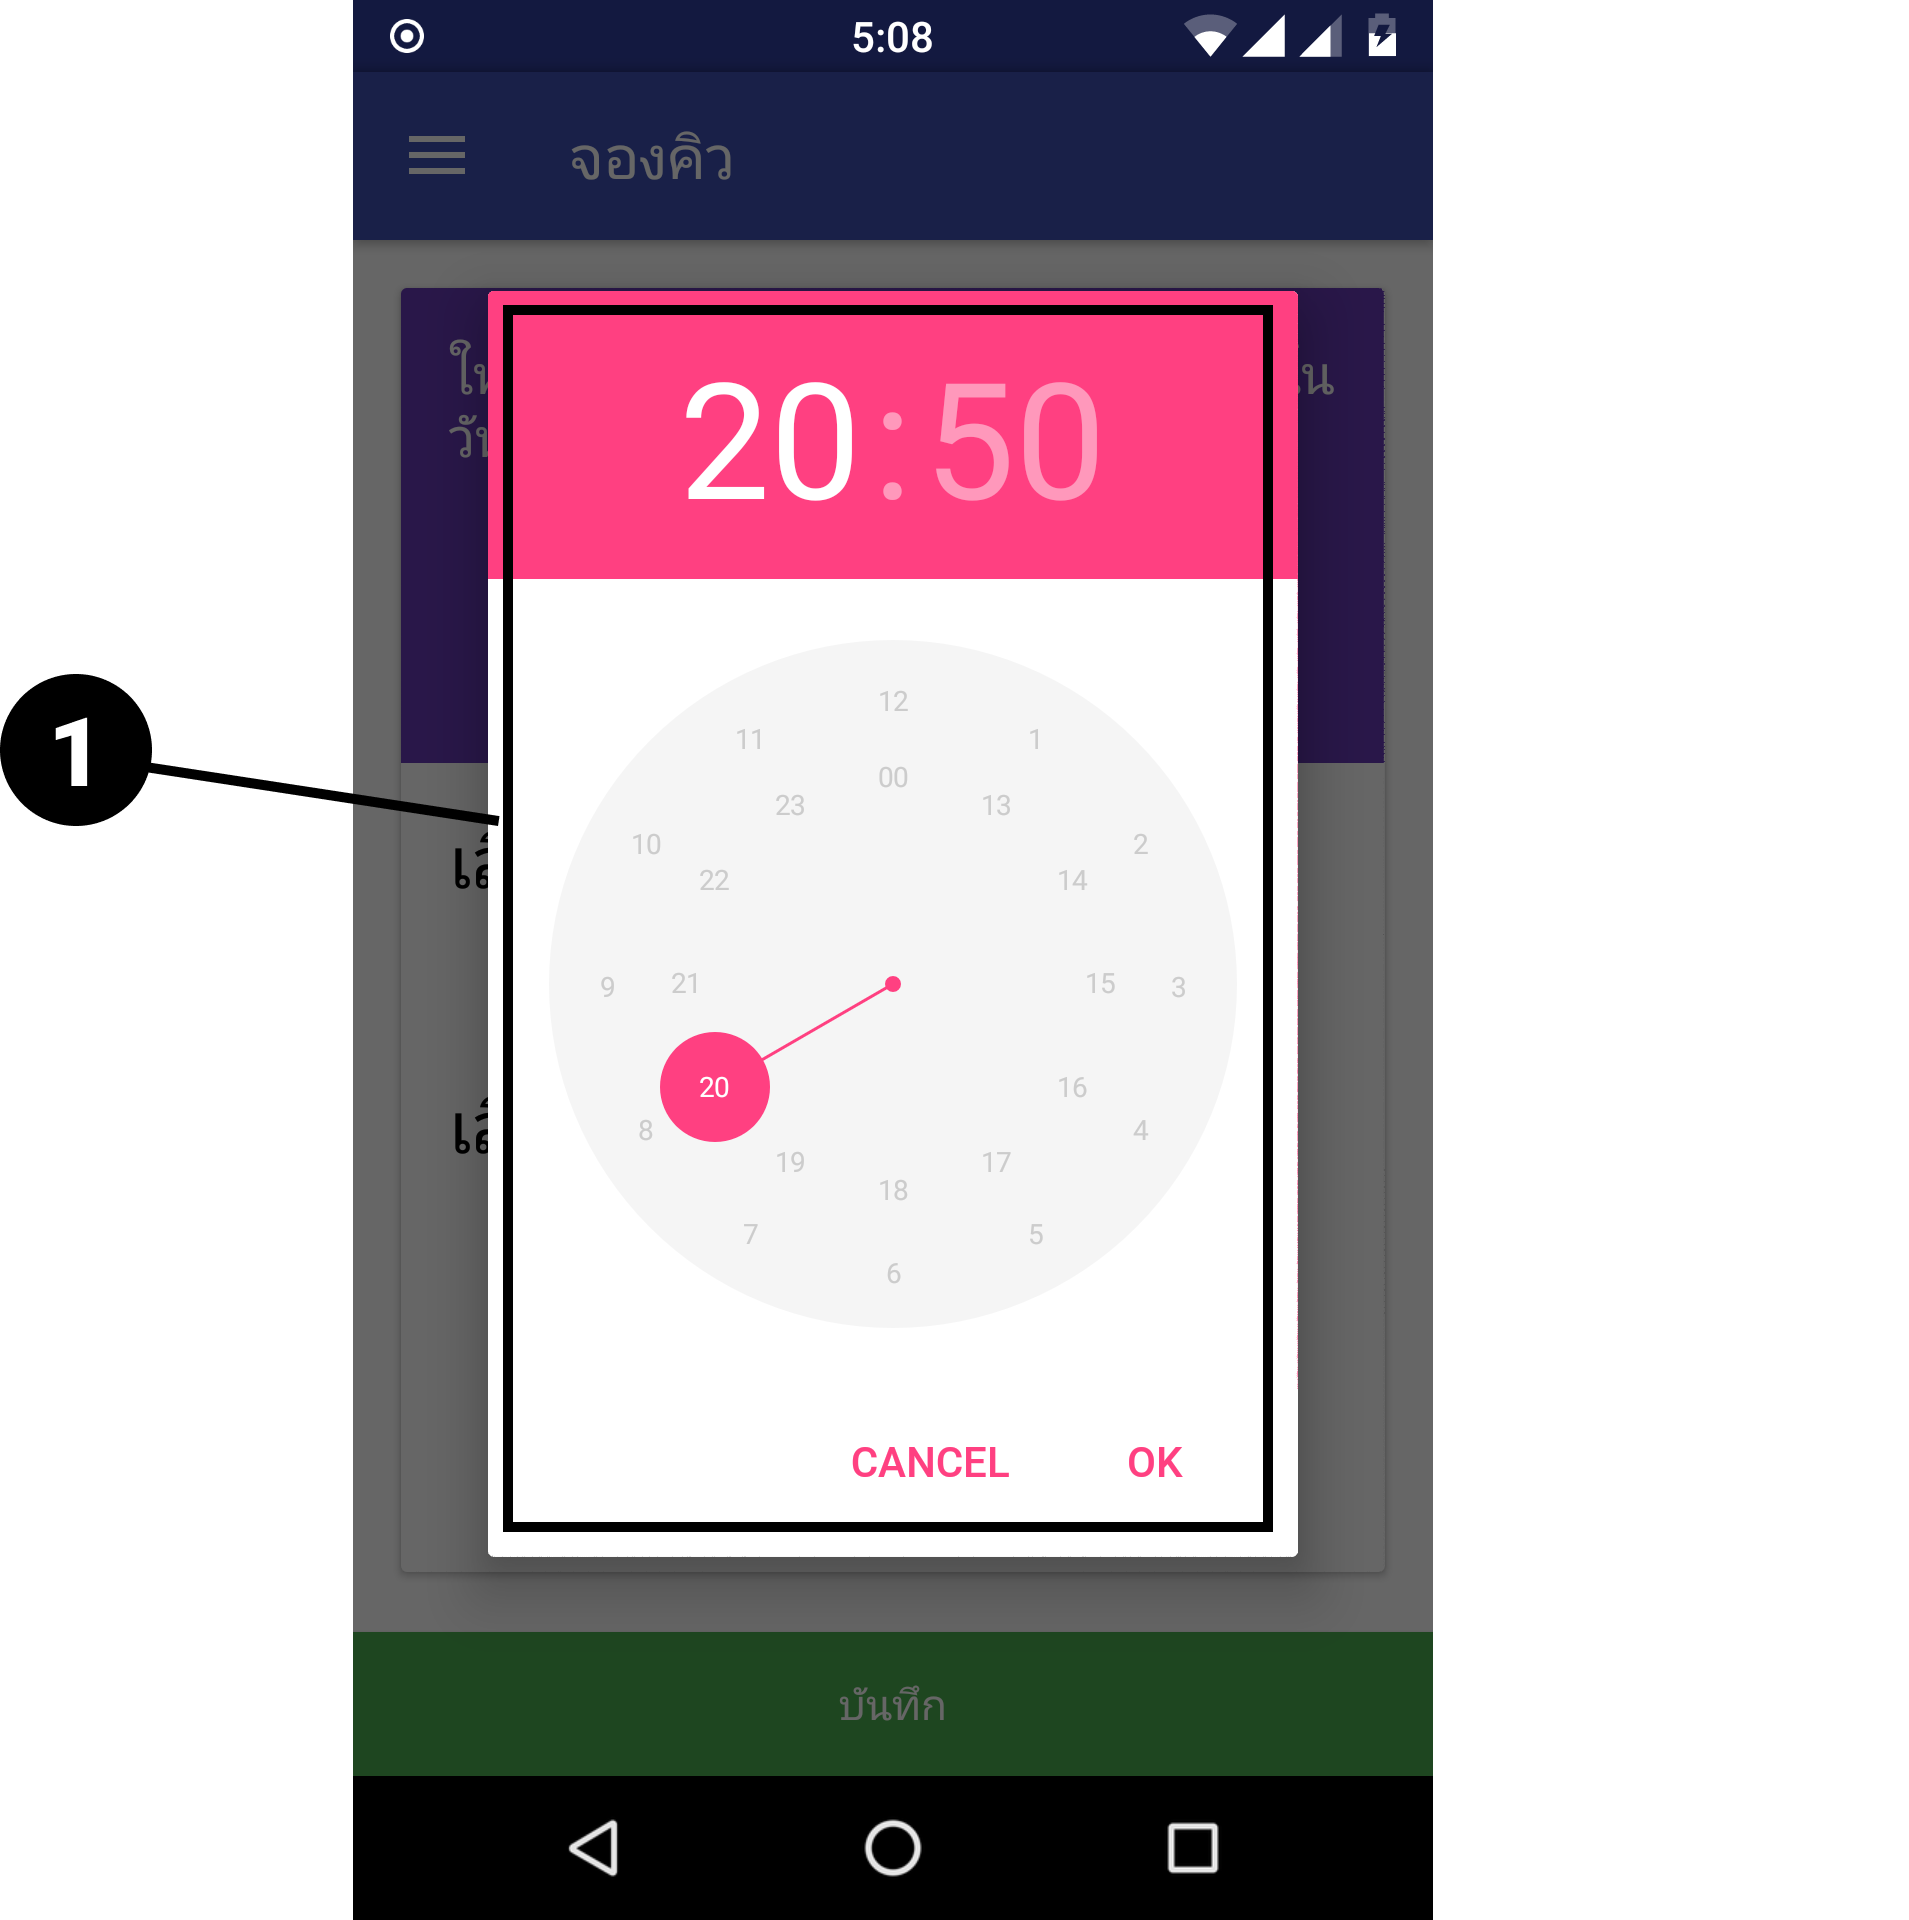
\includegraphics[width=0.5\columnwidth]{Figures/7/Manual/time}
				\caption{หน้าต่างนาฬิกาเลือกเวลาที่ต้องการส่งเอกสาร}
				\label{Fig:time}
			\end{figure}
			จากรูปที่ \ref{Fig:time} สามารถอธิบายการใช้งานได้ดังนี้
			\begin{itemize}[label={--}]
				\item หมายเลข 1 คือ หน้าต่างนาฬิกาเลือกเวลาที่ต้องการส่งเอกสาร 
			\end{itemize}  
		
			\item เมื่อผู้ใช้กดเมนูคำถามที่พบบ่อยระบบจะแสดงหน้าจอคำถามที่พบบ่อย ดังแสดงในรูปที่ \ref{Fig:faq2}
			\begin{figure}[H]
				\centering
				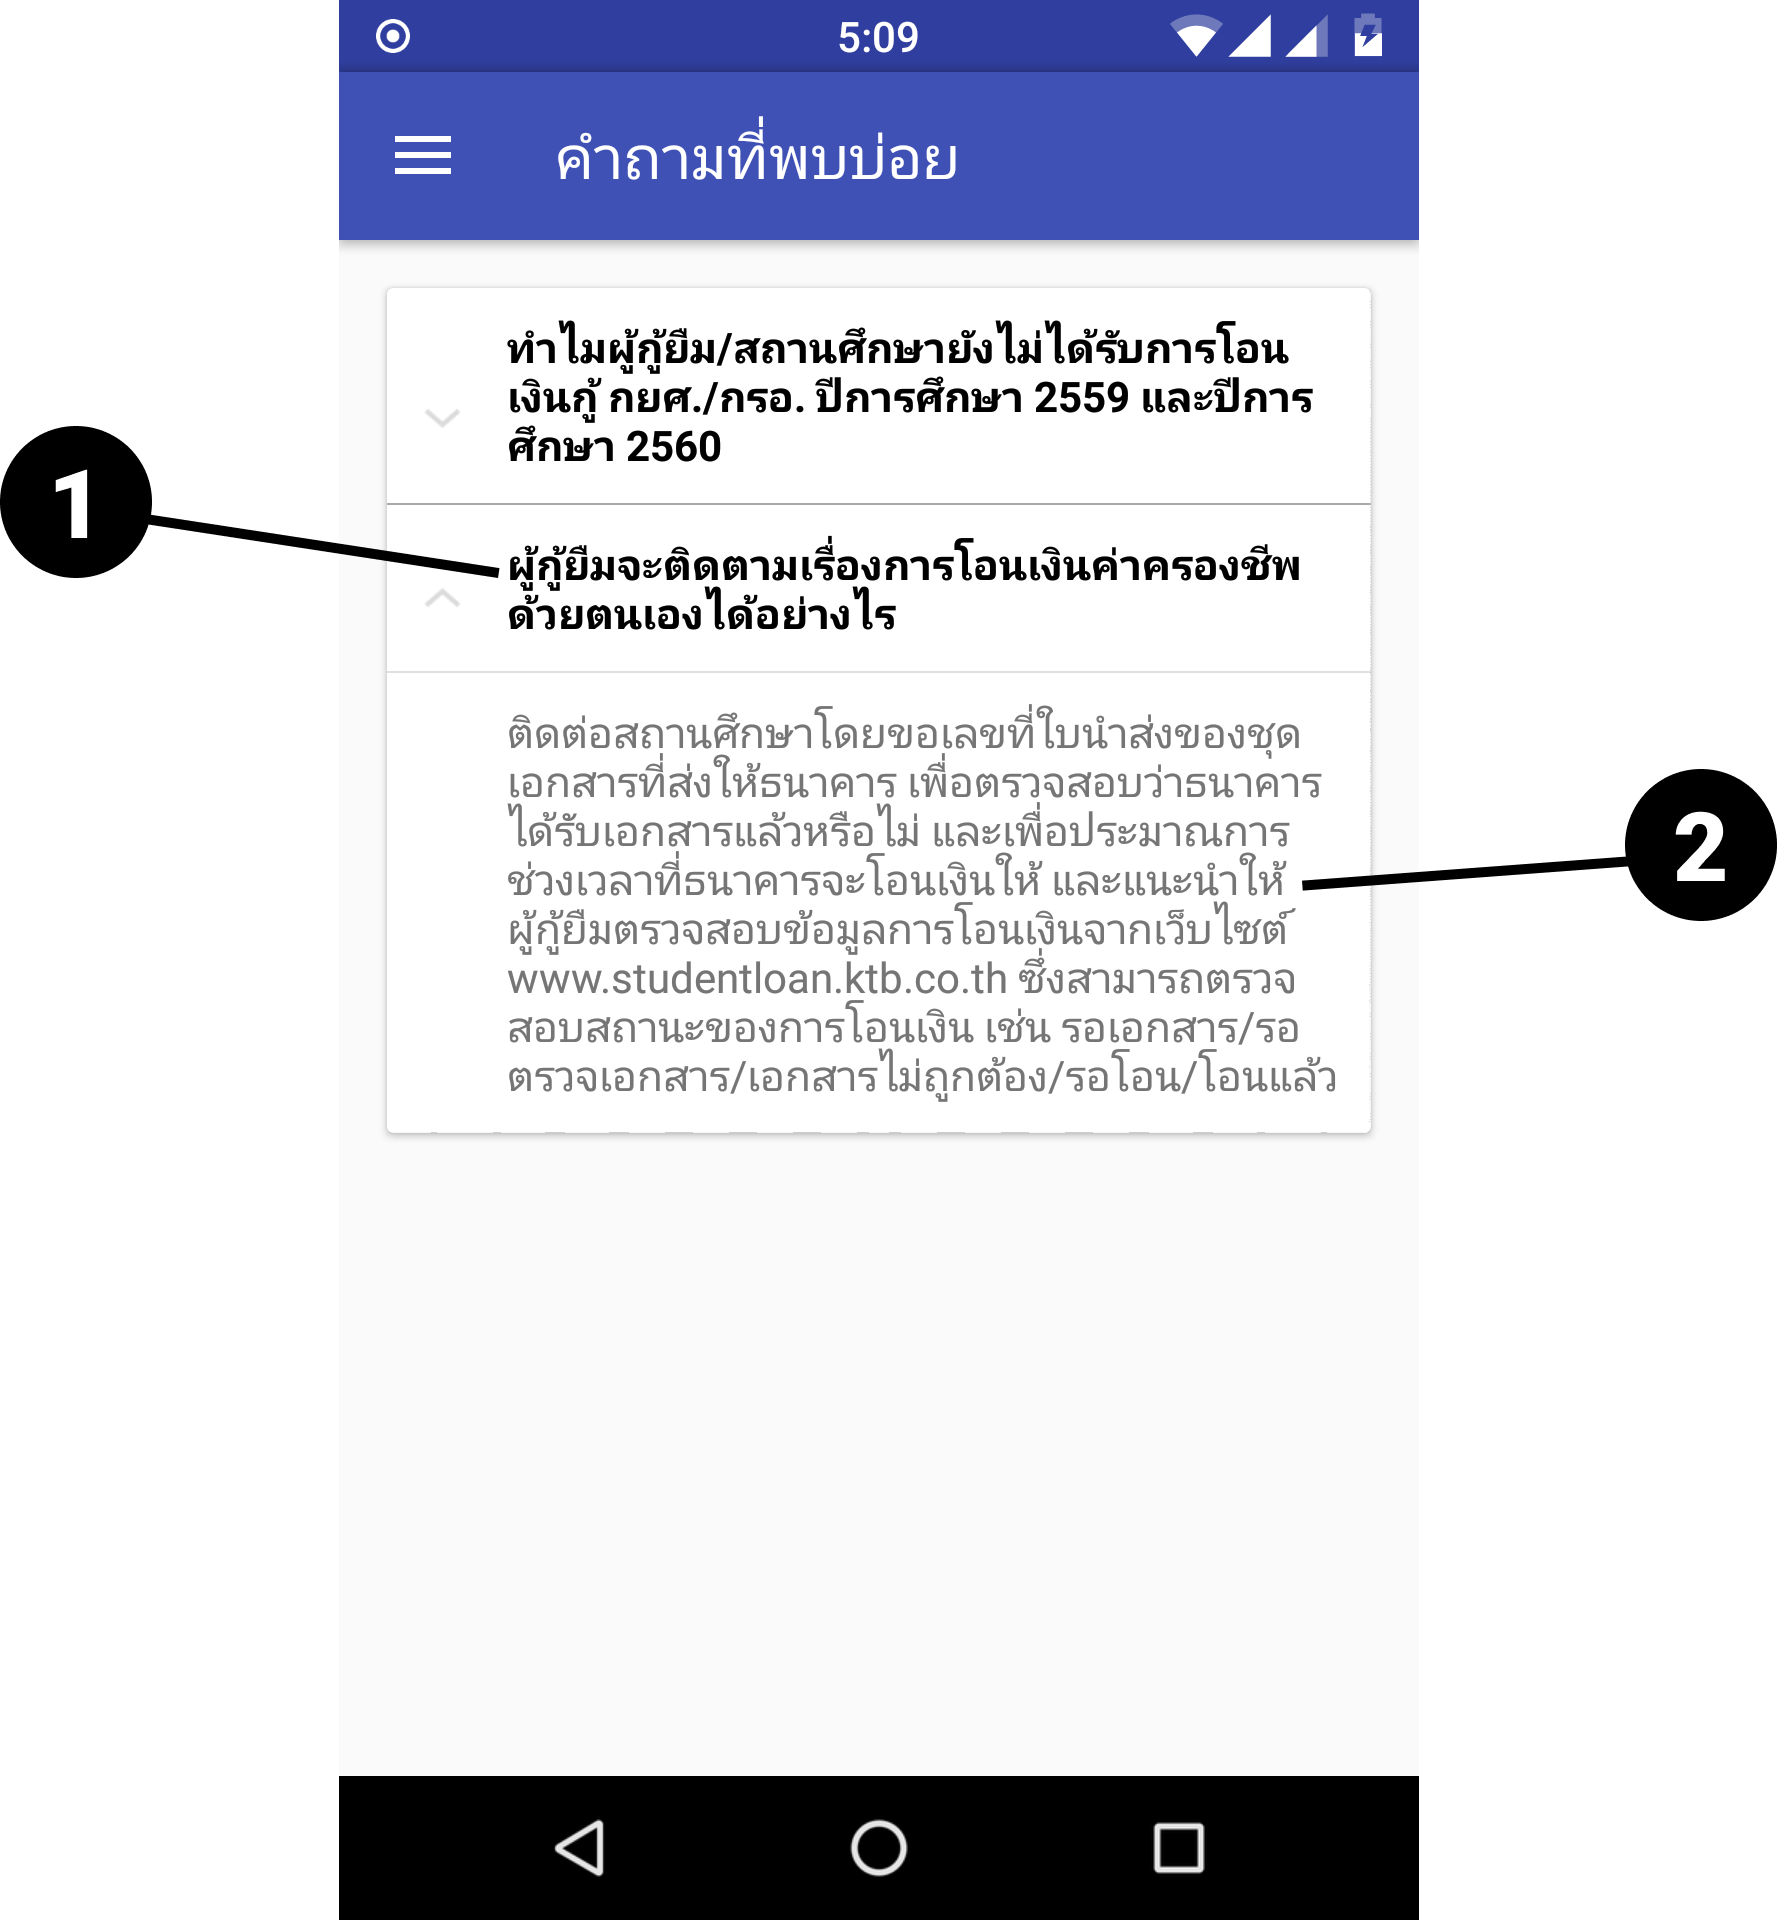
\includegraphics[width=0.5\columnwidth]{Figures/7/Manual/faq2}
				\caption{หน้าจอคำถามที่พบบ่อย}
				\label{Fig:faq2}
			\end{figure}
			จากรูปที่ \ref{Fig:faq2} สามารถอธิบายการใช้งานได้ดังนี้
			\begin{itemize}[label={--}]
				\item หมายเลข 1 คือ คำถาม
				\item หมายเลข 2 คือ คำตอบ
			\end{itemize}  
	
			\item เมื่อผู้ใช้กดปุ่มเมนูเกี่ยวกับเราระบบจะแสดงข้อมูลรายะเอียดของงานพัฒนานักศึกษา คณะวิทยาศาสตร์ มหาวิทยาลัยอุบลราชธานี ดังแสดงในรูปที่ \ref{Fig:about}
			\begin{figure}[H]
				\centering
				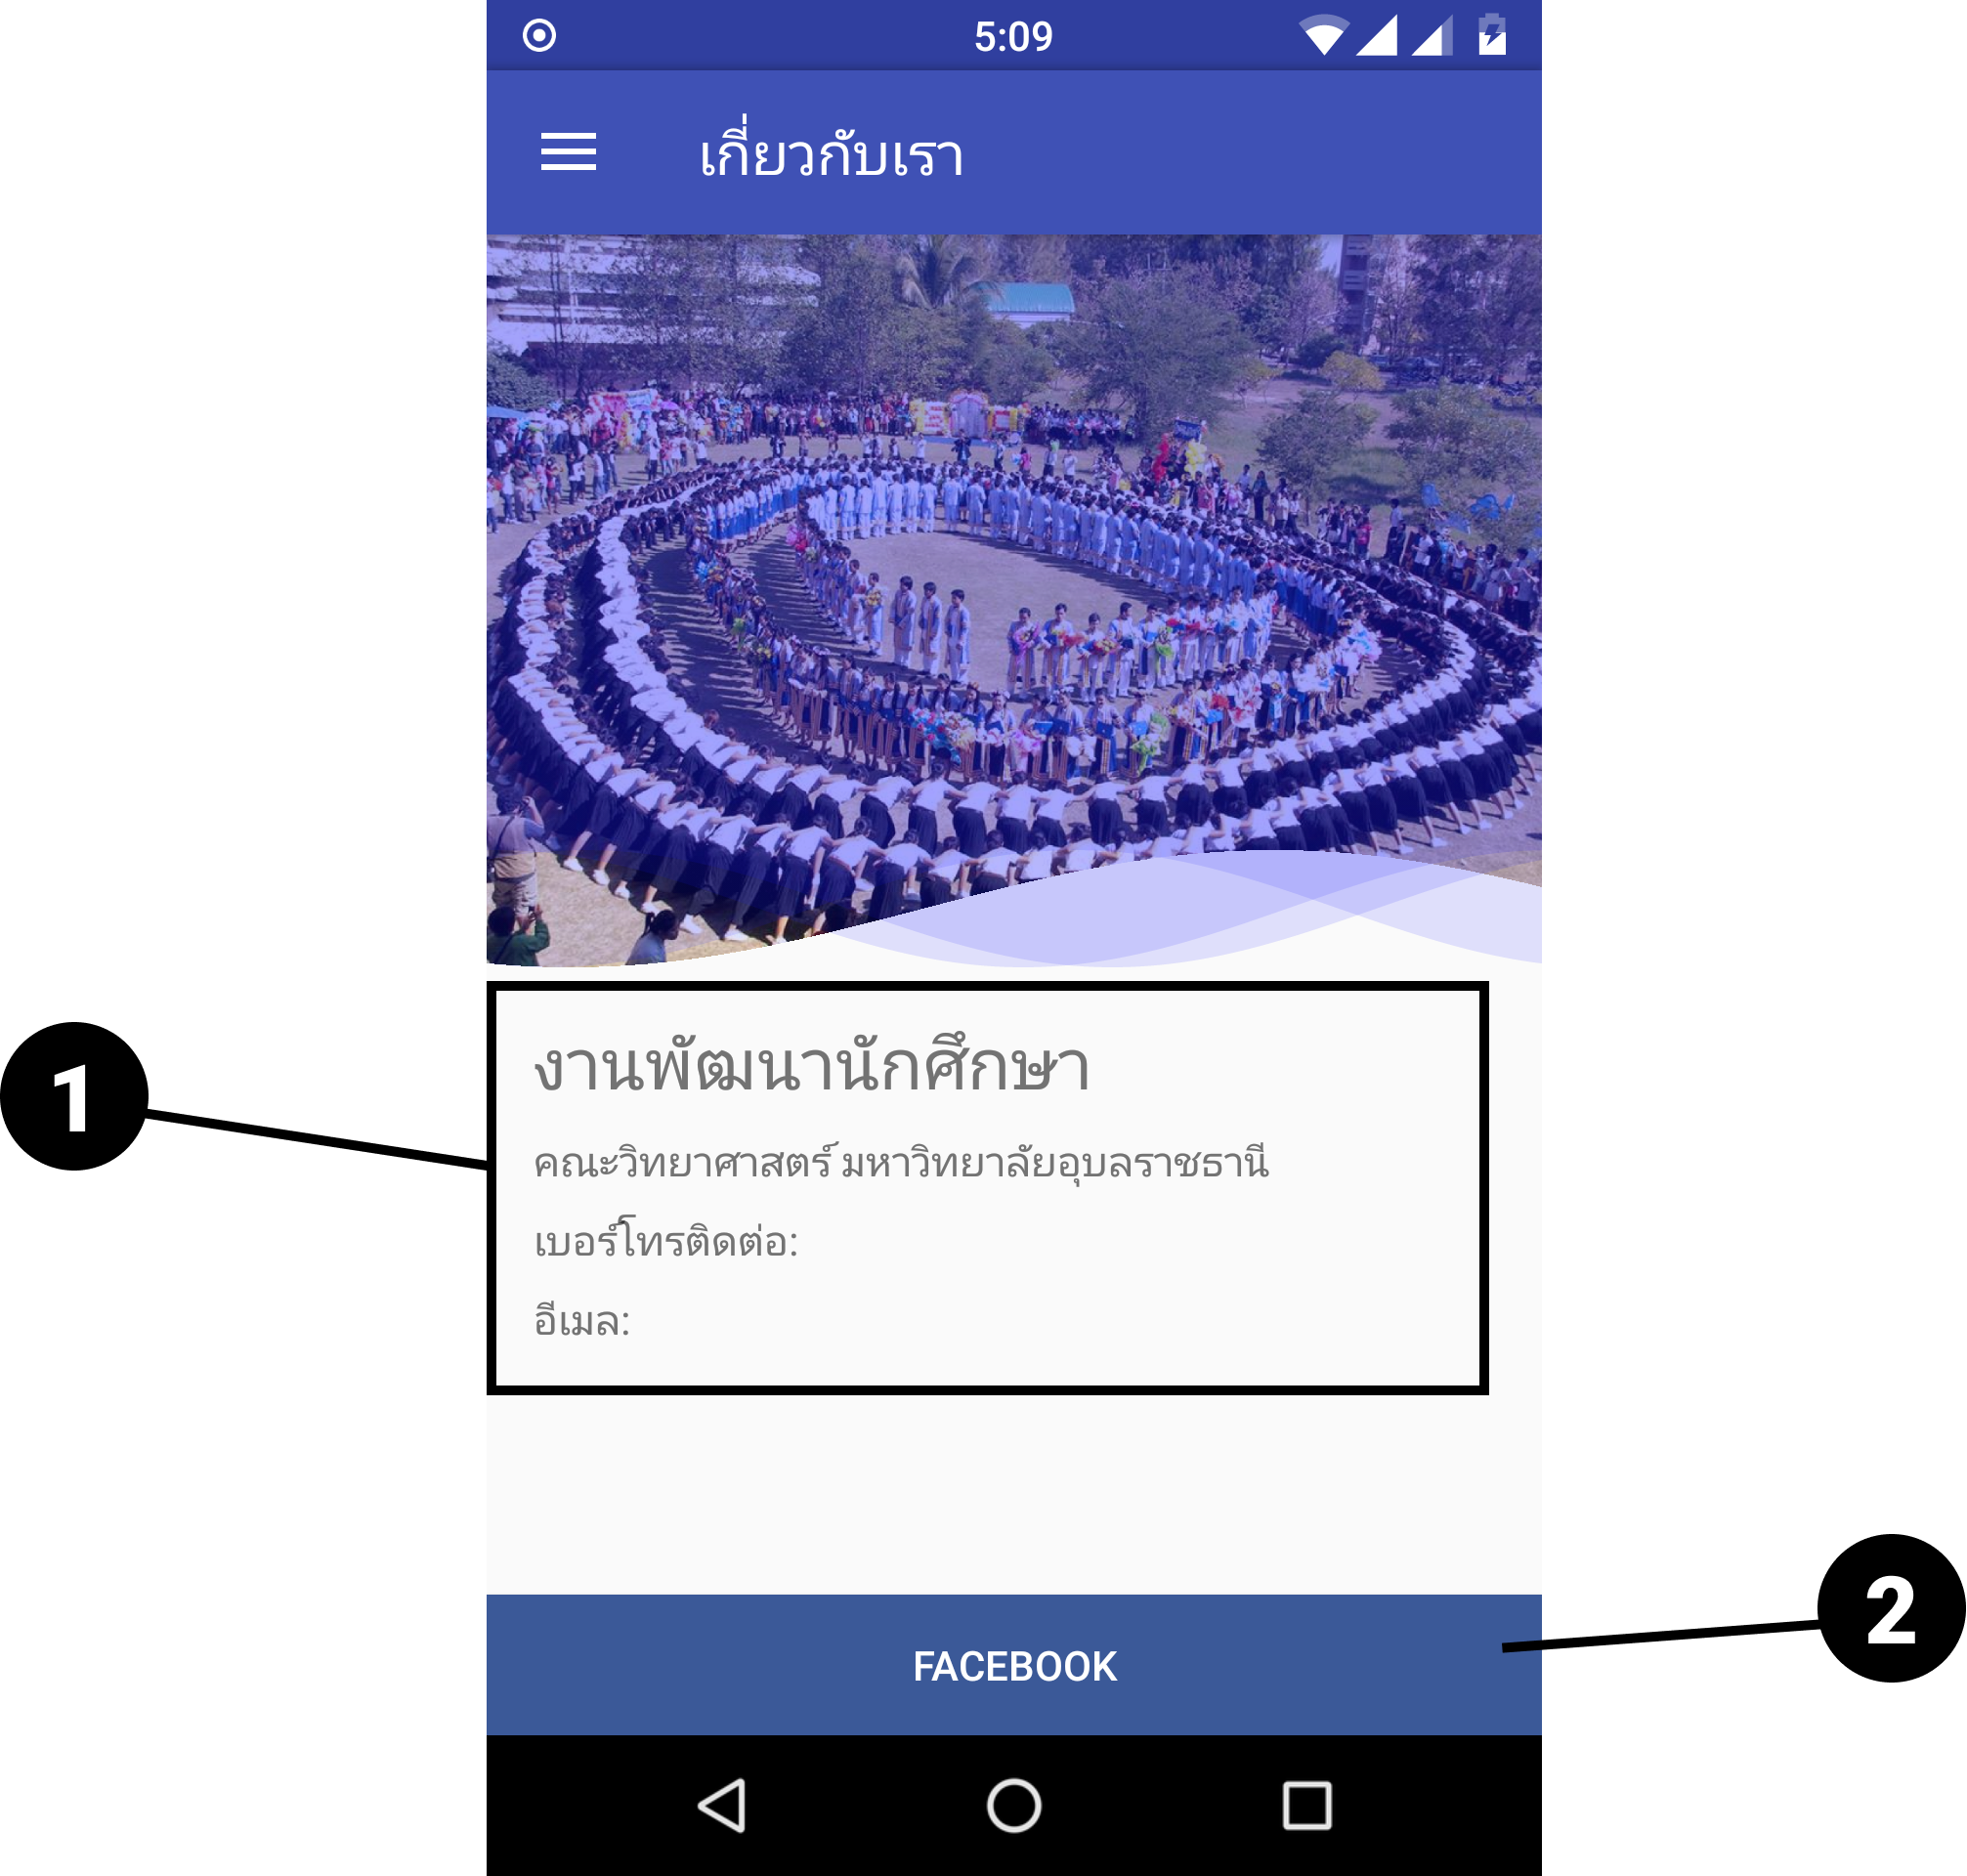
\includegraphics[width=0.5\columnwidth]{Figures/7/Manual/about}
				\caption{หน้าเกี่ยวกับ}
				\label{Fig:about}
			\end{figure}
			จากรูปที่ \ref{Fig:about} สามารถอธิบายการใช้งานได้ดังนี้
			\begin{itemize}[label={--}]
				\item หมายเลข 1 คือ ข้อมูลติดต่องานพัฒนานักศึกษา คณะวิทยาศาสตร์ มหาวิทยาลัยอุบลราชธานี
				\item ปุ่มกดสำหรับเปิดกลุ่มงานพัฒนานักศึกษา คณะวิทยาศาสตร์ มหาวิทยาลัยอุบลราชธานีบน Facebook
			\end{itemize}  
				
		\end{itemize}

\end{enumerate}
